% io-2.tex
% Version of Wed Jun 18 20:15:00 PDT 1997

% Note on formating etype and filetype.
% These are both used as terms and as arguments in MPI routines.
% Their formating depends on the context. As arguments, they should, like
% other arguments to MPI routines, be formatted with \mpiarg.
% As terms or concepts, e.g., talking about etypes within a filetype,
% they should not be formated with \mpiarg.

\chapter{I/O}
\mpitermtitleindex{IO@I/O}
\label{chap:io-2}
\label{sec:io-2}

\section{Introduction}
%=====================
\label{sec:io-intro}

% Different parallel file systems support different interfaces, and
% the lack of a standard portable interface makes it impossible to
% develop a truly portable parallel program.
% It is not feasible to develop large scientific applications
% from scratch for each generation of parallel machine.
% In the scientific world, portability and performance
% are inseparable---a program is not considered truly portable
% unless it not only compiles, but also runs efficiently.
POSIX provides a model of a widely portable file system,
but the portability and optimization needed for parallel I/O
cannot be achieved with
the POSIX interface\mpitermindex{POSIX!model}.
% traditional POSIX.

The significant optimizations required for efficiency
(e.g., grouping \cite{nitzberg:cfs},
collective buffering
\cite{bordawekar:primitives,delrosario:two-phase,nitzberg:thesis,seamons:panda,thakur:jext2phase},
and disk-directed I/O \cite{kotz:diskdir})
can only be implemented
if the parallel I/O system provides a high-level interface supporting
partitioning of file data among processes
and a collective interface
supporting
complete transfers of global data structures between process
memories and files.
In addition, further efficiencies can be gained via support
for asynchronous I/O, strided accesses,
and control over physical file layout on storage devices (disks).
The I/O environment described in this chapter provides these facilities.

Instead of defining
I/O
access modes to express the common patterns
for accessing a shared file (broadcast, reduction, scatter, gather),
we chose another approach
in which data partitioning is expressed using
derived datatypes.
Compared to a limited set of predefined access patterns, 
this approach has the advantage of added flexibility and expressiveness.

\subsection{Definitions}
%-----------------------
\label{subsec:io-2:definitions}
\begin{description}

\item[\mpitermdefni{\MPI/ file}\mpitermdefindex{MPI file@\MPI/ file}:]
An \MPI/ file is an ordered collection of typed data items.
\MPI/ supports random or sequential access to any integral set of these items.
A file is opened collectively by a group of processes.
All collective I/O calls on a file are collective over this group.

\item[\mpitermdef{displacement}:]
A file \mpitermni{displacement} is an absolute byte position
relative to the beginning of a file.
The displacement defines the location where a \mpiterm{view}\mpitermindex{file!view} begins.
Note that a ``file displacement'' is distinct from a ``typemap displacement.''

\item[\mpitermdef{etype}:]
An \mpitermni{etype} (\mpitermni{elementary} datatype\mpitermdefindex{elementary datatype})
is the unit of data access and positioning.
It can be any \MPI/ predefined or derived datatype.
Derived etypes can be constructed
using any of the \MPI/ datatype constructor routines,
provided all resulting typemap displacements are nonnegative
and monotonically increasing.
Data access is performed in etype units,
reading or writing whole data items of type etype.
Offsets are expressed as a count of etypes;
file pointers point to the beginning of etypes.
Depending on context,
the term ``etype'' is used to describe one of three aspects
of an elementary datatype:
a particular \MPI/ type,
a data item of that type,
or the extent of that type.

\item[\mpitermdefni{filetype}\mpitermdefindex{file!filetype}:]
A \mpitermni{filetype} is the basis for partitioning a file among processes
and defines a template for accessing the file.
A filetype is either a single etype or a derived \MPI/ datatype
constructed from multiple instances of the same etype.
In addition,
the extent of any hole in the filetype
must be a multiple of the etype's extent.
The displacements in the typemap of the filetype are not required to be distinct,
but they must be nonnegative and monotonically nondecreasing.

\item[\mpitermdef{view}\mpitermdefindex{file!view}:]
A \mpitermni{view} defines the current set of data visible
and accessible from an open file as an ordered set of etypes.
Each process has its own view of the file,
defined by three quantities:
a displacement, an etype, and a filetype.
The pattern described by a filetype is repeated,
beginning at the displacement, to define the view.
The pattern of repetition is defined to be the same pattern
that \mpifunc{MPI\_TYPE\_CONTIGUOUS} would produce if it were passed
the filetype and an arbitrarily large count.
Figure~\ref{fig:io-filetype} shows how the tiling works; note 
that the filetype in this example must have explicit 
lower and upper bounds set in order for the initial and final holes to be
repeated in the view.
Views can be changed by the user during program execution.
The default view is a linear byte stream
(displacement is zero, etype and filetype equal to \type{MPI\_BYTE}).

\begin{figure}[htpb]
  \centerline{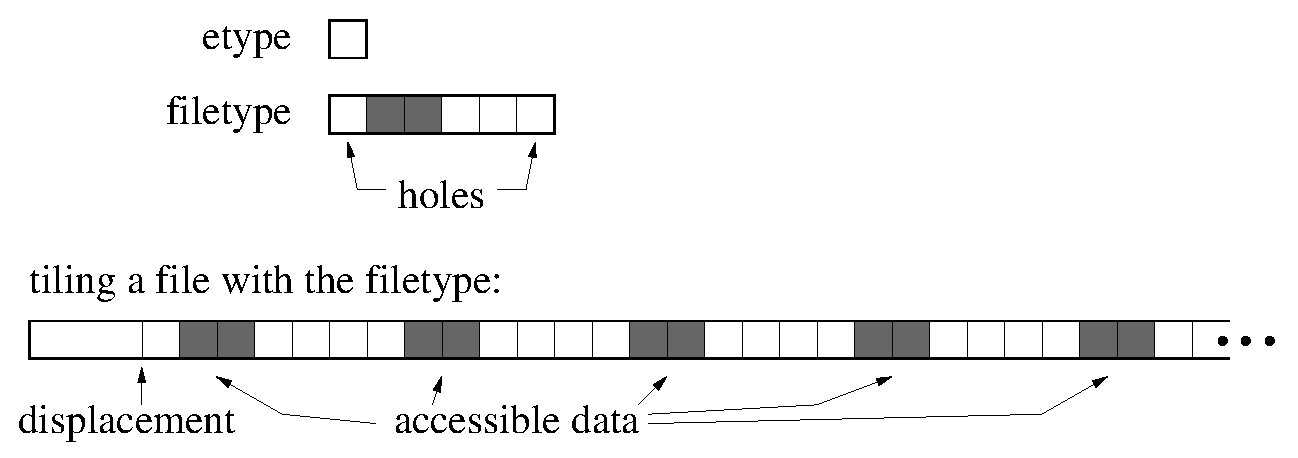
\includegraphics[width=4.0in]{figures/io-filetype}}
  \caption{Etypes and filetypes}
  \label{fig:io-filetype}
\end{figure}

A group of processes can use complementary views to
achieve a global data distribution, such as a scatter/gather pattern
(see Figure~\ref{fig:io-comp-filetypes}).

\begin{figure}[htpb]
  \centerline{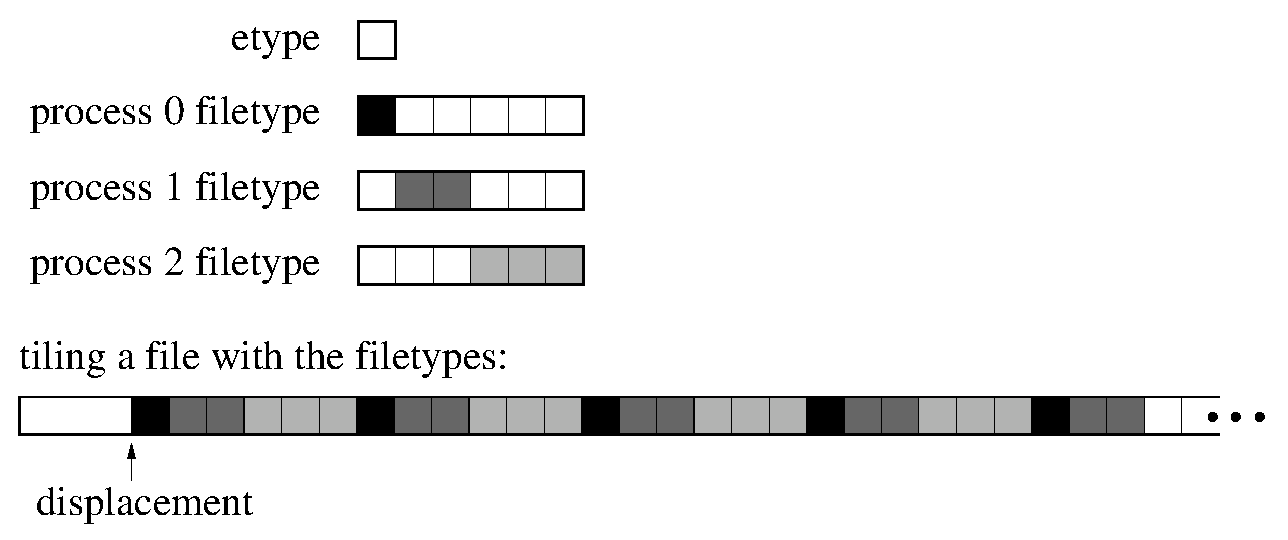
\includegraphics[width=4.0in]{figures/io-comp-filetypes}}
  \caption{Partitioning a file among parallel processes}
  \label{fig:io-comp-filetypes}
\end{figure}

\item[\mpitermdef{offset}\mpitermdefindex{file!offset}:]
An \mpitermni{offset} is a position
in a file
relative to the current view,
expressed as a count of etypes.
Holes in the view's filetype are skipped when calculating this position.
Offset 0 is the location of the first etype visible in the view
(after skipping the displacement and any initial holes in the view).
For example, an offset of 2 for Process 1
in Figure~\ref{fig:io-comp-filetypes} is the position
of the eighth etype in the file after the displacement.
An ``explicit offset'' is an offset that is used as an argument
in explicit data access routines.

\item[\mpitermdefni{file size}\mpitermdefindex{file!size} and \mpitermdef{end of file}\mpitermdefindex{file!end of file}:]
The \mpitermni{size} of an \MPI/ file is measured in bytes from the 
beginning of the file.  A newly created file has a size of zero 
bytes.  Using the size as an absolute displacement gives 
the position of the byte immediately following the last byte in 
the file.  For any given view, the \mpitermni{end of file} is the 
offset of the first etype accessible in the current view starting
after the last byte in the file.

\item[\mpitermdefni{file pointer}\mpitermdefindex{file!pointer}:]
A \mpitermni{file pointer} is an implicit offset maintained by \MPI/.
``Individual file pointers'' are file pointers that are local to
each process that opened the file.
A ``shared file pointer'' is a file pointer that is shared by
the group of processes that opened the file.

\item[\mpitermdefni{file handle}\mpitermdefindex{file!handle}:]
A \mpitermni{file handle} is an opaque object created by \mpifunc{MPI\_FILE\_OPEN}
and freed by \mpifunc{MPI\_FILE\_CLOSE}.
All operations on an open file
reference the file through the file handle.

\end{description}

\section{File Manipulation}
\mpitermtitleindex{file!manipulation}
%==========================
\label{sec:io-filecntl}

\subsection{Opening a File}
%--------------------------
\label{sec:io-filecntl-open}

\cdeclindex{MPI\_Info}%
\cdeclmainindex{MPI\_File}\cdeclmainindex{TYPE(MPI\_File)}%
\begin{funcdef}{MPI\_FILE\_OPEN}{(\mbox{comm}, \mbox{filename}, \mbox{amode}, \mbox{info}, \mbox{fh})}
\funcarg{\IN}{comm}{communicator (handle)}
\funcarg{\IN}{filename}{name of file to open (string)}
\funcarg{\IN}{amode}{file access mode (integer)}
\funcarg{\IN}{info}{info object (handle)}
\funcarg{\OUT}{fh}{new file handle (handle)}
\end{funcdef}
\mpibindmain{MPI\_File\_open}{(\gb{}MPI\_Comm~comm, const~char~*filename, int~amode, MPI\_Info~info, MPI\_File~*fh)}
\mpifnewbindmain{MPI\_File\_open}{(comm, filename, amode, info, fh, ierror) \fargs TYPE(MPI\_Comm), INTENT(IN)\ ::\ \mbox{comm}\fnarg{}CHARACTER(LEN=*), INTENT(IN)\ ::\ \mbox{filename}\fnarg{}INTEGER, INTENT(IN)\ ::\ \mbox{amode}\fnarg{}TYPE(MPI\_Info), INTENT(IN)\ ::\ \mbox{info}\fnarg{}TYPE(MPI\_File), INTENT(OUT)\ ::\ \mbox{fh}\fnfinalarg{}INTEGER, OPTIONAL, INTENT(OUT)\ ::\ \mbox{ierror}}
\mpifbindmain{MPI\_FILE\_OPEN}{(COMM, FILENAME, AMODE, INFO, FH, IERROR) \fargs INTEGER \mbox{COMM}, \mbox{AMODE}, \mbox{INFO}, \mbox{FH}, \mbox{IERROR}\fnfinalarg{}CHARACTER*(*) \mbox{FILENAME}}

\mpifunc{MPI\_FILE\_OPEN} opens the file identified by the file name
\mpiarg{filename} on all processes in the \mpiarg{comm} communicator group.
\mpifunc{MPI\_FILE\_OPEN} is a collective routine:
all processes must provide the same value for \mpiarg{amode},
and all processes must provide \mpiarg{filename}s that
reference the same file.
(Values for \mpiarg{info} may vary.)
\mpiarg{comm} must be an intra-communicator;
it is erroneous to pass an inter-communicator to \mpifunc{MPI\_FILE\_OPEN}.
Errors in \mpifunc{MPI\_FILE\_OPEN} are raised 
using the default file error handler\mpitermindex{error handling!default file error handler}
(see \sectionref{sec:io-errhandlers}).
When using the \wpm{}\mpitermindex{MPI process initialization@\MPI/ process initialization!\wpm}\mpitermindex{\wpm} (Section~\ref{sec:dynamic:introduction}),
a process can open a file independently of other processes
by using the \mpiconst{MPI\_COMM\_SELF} communicator.
Applications using the \spm{} (Section~\ref{sec:model_sessions})\mpitermindex{MPI process initialization@\MPI/ process initialization!\spm}\mpitermindex{\spm} can achieve the same result using communicators created from the \mpistring{mpi://SELF} process set.
The file handle returned, \mpiarg{fh},
can subsequently be used to access the file until the file is
closed using \mpifunc{MPI\_FILE\_CLOSE}.
Before calling \mpifunc{MPI\_FINALIZE},
the user is required to close (via \mpifunc{MPI\_FILE\_CLOSE})
all files that were opened with \mpifunc{MPI\_FILE\_OPEN}.
Note that the communicator \mpiarg{comm} is unaffected by calls to \mpifunc{MPI\_FILE\_OPEN}
and continues to be usable in all \MPI/ routines (e.g., \mpifunc{MPI\_SEND}).
Furthermore, the use of \mpiarg{comm} will not interfere with I/O behavior.

The format for specifying the file name in the \mpiarg{filename}
argument is implementation dependent
and must be documented by the implementation.

\begin{implementors}
An implementation may require that \mpiarg{filename} include
a string or strings specifying additional information about the file.
Examples include the type of filesystem (e.g., a prefix of \code{ufs:}),
a remote hostname (e.g., a prefix of \code{machine.univ.edu:}),
or a file password (e.g., a suffix of \code{/PASSWORD=SECRET}).
\end{implementors}

\begin{users}
On some implementations of \MPI/,
the file namespace may not be identical from all processes of all applications.
For example,
``\code{/tmp/foo}'' may denote different files on different processes,
or a single file may have many names, dependent on process location.
The user is responsible for ensuring that a single file
is referenced by the \mpiarg{filename} argument,
as it may be impossible for an implementation to detect
this type of namespace error.
\end{users}

Initially, all processes view the file as a linear byte stream,
and each process views data in its own native representation
(no data representation conversion is performed).
(POSIX files are linear byte streams in the native representation.)
The file view can be changed
via the \mpifunc{MPI\_FILE\_SET\_VIEW} routine\mpitermindex{POSIX!I/O}.

The following access modes are supported
(specified in \mpiarg{amode}, a bit vector created by \mpicode{OR} with one or more of the following
integer constants):
\begin{constlist}
\constmainitem{MPI\_MODE\_RDONLY}{read only}
\constmainitem{MPI\_MODE\_RDWR}{reading and writing}
\constmainitem{MPI\_MODE\_WRONLY}{write only}
\constmainitem{MPI\_MODE\_CREATE}{create the file if it does not exist}
\constmainitem{MPI\_MODE\_EXCL}{error if creating file that already exists}
\constmainitem{MPI\_MODE\_DELETE\_ON\_CLOSE}{delete file on close}
\constmainitem{MPI\_MODE\_UNIQUE\_OPEN}{file will not be opened concurrently
   elsewhere}
\constmainitem{MPI\_MODE\_SEQUENTIAL}{file will only be accessed sequentially}
\constmainitem{MPI\_MODE\_APPEND}{set initial position of all file pointers to end of file}
\end{constlist}

\begin{users}
C users can use bit vector \mpicode{OR} ($\mid$) to combine these constants;
Fortran 90 users can use the bit vector \code{IOR} intrinsic.
Fortran 77 users can use (nonportably) bit vector \code{IOR}
on systems that support it.
Alternatively,
Fortran users can portably use integer addition to \mpicode{OR} the constants
(each constant should appear at most once in the addition.).
\end{users}

\begin{implementors}
The values of these constants must be defined such that
the bitwise \mpicode{OR} and the sum of any distinct set
of these constants is equivalent.
\end{implementors}

The modes \mpiconst{MPI\_MODE\_RDONLY}, \mpiconst{MPI\_MODE\_RDWR}, 
\mpiconst{MPI\_MODE\_WRONLY},
\mpiconst{MPI\_MODE\_CREATE}, and \mpiconst{MPI\_MODE\_EXCL} have identical semantics
to their POSIX counterparts \cite{posix-1003.1}\mpitermindex{POSIX!I/O}.
Exactly one of \mpiconst{MPI\_MODE\_RDONLY}, \mpiconst{MPI\_MODE\_RDWR}, 
or \mpiconst{MPI\_MODE\_WRONLY},
must be specified.
It is erroneous to specify \mpiconst{MPI\_MODE\_CREATE} 
or \mpiconst{MPI\_MODE\_EXCL}
in conjunction with \mpiconst{MPI\_MODE\_RDONLY};
it is erroneous to specify \mpiconst{MPI\_MODE\_SEQUENTIAL}
together with \mpiconst{MPI\_MODE\_RDWR}.


The \mpiconst{MPI\_MODE\_DELETE\_ON\_CLOSE} mode causes the file to be deleted
(equivalent to performing an \mpifunc{MPI\_FILE\_DELETE})
when the file is closed.

The \mpiconst{MPI\_MODE\_UNIQUE\_OPEN} mode allows an implementation to
optimize access by eliminating the overhead of file locking.
It is erroneous to open a file in this mode unless the file will
not be opened concurrently elsewhere.

\begin{users}
For \mpiconst{MPI\_MODE\_UNIQUE\_OPEN}, \emph{not opened elsewhere} includes
both inside and outside the \MPI/ environment.
In particular, one needs to be aware of potential external events
that may open files (e.g., automated backup facilities).
When \mpiconst{MPI\_MODE\_UNIQUE\_OPEN} is specified,
the user is responsible for ensuring that no such external events take place.
\end{users}

The \mpiconst{MPI\_MODE\_SEQUENTIAL} mode allows an implementation to
optimize access to some sequential devices (tapes and network streams).
It is erroneous to attempt nonsequential access to a
file that has been opened in this mode.

Specifying \mpiconst{MPI\_MODE\_APPEND} only guarantees that all shared and individual
file pointers are positioned at the initial end of file when \mpifunc{MPI\_FILE\_OPEN}
returns.
Subsequent positioning of file pointers is application dependent.
In particular, the implementation does not ensure that all writes are
appended.

Errors related to the access mode are raised
in the class \errormain{MPI\_ERR\_AMODE}.

The \mpiarg{info} argument is used to provide information
regarding file access patterns and file system specifics
(see \sectionref{sec:io-info}).
The constant \mpiconst{MPI\_INFO\_NULL}
can be used when no info needs to be specified.
\begin{users}
Some file attributes are inherently implementation dependent
(e.g., file permissions).
These attributes must be set using either
the \mpiarg{info} argument or facilities outside the scope of \MPI/.
\end{users}

Files are opened by default using nonatomic mode file consistency semantics
(see \sectionref{sec:io-filecntl-atomicity}).
The more stringent atomic mode consistency semantics,
required for atomicity of conflicting accesses,
can be set using \mpifunc{MPI\_FILE\_SET\_ATOMICITY}.

\subsection{Closing a File}
%--------------------------
\label{sec:io-filecntl-close}

\cdeclindex{MPI\_File}%
\begin{funcdef}{MPI\_FILE\_CLOSE}{(\mbox{fh})}
\funcarg{\INOUT}{fh}{file handle (handle)}
\end{funcdef}
\mpibindmain{MPI\_File\_close}{(\gb{}MPI\_File~*fh)}
\mpifnewbindmain{MPI\_File\_close}{(fh, ierror) \fargs TYPE(MPI\_File), INTENT(INOUT)\ ::\ \mbox{fh}\fnfinalarg{}INTEGER, OPTIONAL, INTENT(OUT)\ ::\ \mbox{ierror}}
\mpifbindmain{MPI\_FILE\_CLOSE}{(FH, IERROR) \fargs \fnfinalarg{}INTEGER \mbox{FH}, \mbox{IERROR}}

\mpifunc{MPI\_FILE\_CLOSE} first synchronizes file state
(equivalent to performing an \mpifunc{MPI\_FILE\_SYNC}),
then closes the file associated with \mpiarg{fh}.
The file is deleted if it was opened with access mode
\mpiconst{MPI\_MODE\_DELETE\_ON\_CLOSE}
(equivalent to performing an \mpifunc{MPI\_FILE\_DELETE}).
\mpifunc{MPI\_FILE\_CLOSE} is a collective routine over the group associated with the file.

\begin{users}
If the file is deleted on close, and there are
other processes currently accessing the file,
the status of the file and the behavior of future accesses
by these processes are implementation dependent.
\end{users}

The user is responsible for ensuring that all outstanding
nonblocking requests and split collective
operations associated with \mpiarg{fh}
made by a process have completed
before that process calls \mpifunc{MPI\_FILE\_CLOSE}.

The \mpifunc{MPI\_FILE\_CLOSE} routine deallocates the file handle object
and sets \mpiarg{fh} to \mpiconst{MPI\_FILE\_NULL}.

\subsection{Deleting a File}
%---------------------------
\label{sec:io-filecntl-delete}

\cdeclindex{MPI\_Info}%
\begin{funcdef}{MPI\_FILE\_DELETE}{(\mbox{filename}, \mbox{info})}
\funcarg{\IN}{filename}{name of file to delete (string)}
\funcarg{\IN}{info}{info object (handle)}
\end{funcdef}
\mpibindmain{MPI\_File\_delete}{(\gb{}const~char~*filename, MPI\_Info~info)}
\mpifnewbindmain{MPI\_File\_delete}{(filename, info, ierror) \fargs CHARACTER(LEN=*), INTENT(IN)\ ::\ \mbox{filename}\fnarg{}TYPE(MPI\_Info), INTENT(IN)\ ::\ \mbox{info}\fnfinalarg{}INTEGER, OPTIONAL, INTENT(OUT)\ ::\ \mbox{ierror}}
\mpifbindmain{MPI\_FILE\_DELETE}{(FILENAME, INFO, IERROR) \fargs CHARACTER*(*) \mbox{FILENAME}\fnfinalarg{}INTEGER \mbox{INFO}, \mbox{IERROR}}

\mpifunc{MPI\_FILE\_DELETE} deletes the file
identified by the file name \mpiarg{filename}.
If the file does not exist, \mpifunc{MPI\_FILE\_DELETE} raises an
error of class \errormain{MPI\_ERR\_NO\_SUCH\_FILE}.

The \mpiarg{info} argument can be used to provide information
regarding file system specifics
(see \sectionref{sec:io-info}).
The constant \mpiconst{MPI\_INFO\_NULL}
refers to the null info, and
can be used when no info needs to be specified.

If a process currently has the file open,
the behavior of any access to the file
(as well as the behavior of any outstanding accesses)
is implementation dependent.
In addition, whether an open file is deleted or not is also
implementation dependent.
If the file is not deleted,
an error in the class
\errormain{MPI\_ERR\_FILE\_IN\_USE} or \errormain{MPI\_ERR\_ACCESS} will be raised.
Errors are raised 
using the default file error handler\mpitermindex{error handling!default file error handler}
(see \sectionref{sec:io-errhandlers}).

\subsection{Resizing a File}
%---------------------------
\label{sec:io-filecntl-resize}

\cdeclindex{MPI\_File}%
\cdeclindex{MPI\_Offset}%
\begin{funcdef}{MPI\_FILE\_SET\_SIZE}{(\mbox{fh}, \mbox{size})}
\funcarg{\INOUT}{fh}{file handle (handle)}
\funcarg{\IN}{size}{size to truncate or expand file (integer)}
\end{funcdef}
\mpibindmain{MPI\_File\_set\_size}{(\gb{}MPI\_File~fh, MPI\_Offset~size)}
\mpifnewbindmain{MPI\_File\_set\_size}{(fh, size, ierror) \fargs TYPE(MPI\_File), INTENT(IN)\ ::\ \mbox{fh}\fnarg{}INTEGER(KIND=MPI\_OFFSET\_KIND), INTENT(IN)\ ::\ \mbox{size}\fnfinalarg{}INTEGER, OPTIONAL, INTENT(OUT)\ ::\ \mbox{ierror}}
\mpifbindmain{MPI\_FILE\_SET\_SIZE}{(FH, SIZE, IERROR) \fargs INTEGER \mbox{FH}, \mbox{IERROR}\fnfinalarg{}INTEGER(KIND=MPI\_OFFSET\_KIND) \mbox{SIZE}}

\mpifunc{MPI\_FILE\_SET\_SIZE} resizes the file
associated with the file handle \mpiarg{fh}.
\mpiarg{size} is measured in bytes from the beginning of the file.
\mpifunc{MPI\_FILE\_SET\_SIZE} is collective over the group associated with the file;
all processes in the group must pass identical values for \mpiarg{size}.

If \mpiarg{size} is smaller than the current file size,
the file is truncated at the position defined by \mpiarg{size}.
The implementation is free to deallocate file blocks located
beyond this position.

If \mpiarg{size} is larger than the current file size,
the file size becomes \mpiarg{size}.
Regions of the file that have been previously written are unaffected.
The values of data in the new regions in the file (those
locations with displacements between old file size and \mpiarg{size})
are undefined.
It is implementation dependent whether the \mpifunc{MPI\_FILE\_SET\_SIZE} routine
allocates file space---use \mpifunc{MPI\_FILE\_PREALLOCATE}
to force file space to be reserved.

\mpifunc{MPI\_FILE\_SET\_SIZE} does not affect the individual file pointers
or the shared file pointer.
If \mpiconst{MPI\_MODE\_SEQUENTIAL} mode was specified when the file was opened,
it is erroneous to call this routine.

\begin{users}
It is possible for the file pointers to point beyond the end of file
after a \mpifunc{MPI\_FILE\_SET\_SIZE} operation truncates a file.
This is valid, and equivalent to seeking beyond the current end of file.
\end{users}

All nonblocking requests
and split collective operations
on \mpiarg{fh} must be completed
before calling \mpifunc{MPI\_FILE\_SET\_SIZE}.
Otherwise, calling \mpifunc{MPI\_FILE\_SET\_SIZE} is erroneous.
As far as consistency semantics are concerned,
\mpifunc{MPI\_FILE\_SET\_SIZE} is a write operation
that conflicts with operations that access bytes
at displacements between the old and new file sizes
(see \sectionref{sec:io-filecntl-atomicity}).

\subsection{Preallocating Space for a File}
%------------------------------------------
\label{sec:io-filecntl-preallocate}

\cdeclindex{MPI\_File}%
\cdeclindex{MPI\_Offset}%
\begin{funcdef}{MPI\_FILE\_PREALLOCATE}{(\mbox{fh}, \mbox{size})}
\funcarg{\INOUT}{fh}{file handle (handle)}
\funcarg{\IN}{size}{size to preallocate file (integer)}
\end{funcdef}
\mpibindmain{MPI\_File\_preallocate}{(\gb{}MPI\_File~fh, MPI\_Offset~size)}
\mpifnewbindmain{MPI\_File\_preallocate}{(fh, size, ierror) \fargs TYPE(MPI\_File), INTENT(IN)\ ::\ \mbox{fh}\fnarg{}INTEGER(KIND=MPI\_OFFSET\_KIND), INTENT(IN)\ ::\ \mbox{size}\fnfinalarg{}INTEGER, OPTIONAL, INTENT(OUT)\ ::\ \mbox{ierror}}
\mpifbindmain{MPI\_FILE\_PREALLOCATE}{(FH, SIZE, IERROR) \fargs INTEGER \mbox{FH}, \mbox{IERROR}\fnfinalarg{}INTEGER(KIND=MPI\_OFFSET\_KIND) \mbox{SIZE}}

\mpifunc{MPI\_FILE\_PREALLOCATE} ensures that storage space is
allocated for the first \mpiarg{size} bytes of the file
associated with \mpiarg{fh}. 
\mpifunc{MPI\_FILE\_PREALLOCATE} is collective over the group associated with the file;
all processes in the group must pass identical values for \mpiarg{size}.
Regions of the file that have previously been written are unaffected.
For newly allocated regions of the file, \mpifunc{MPI\_FILE\_PREALLOCATE}
has the same effect as writing undefined data.
If \mpiarg{size} is larger than the current file size,
the file size increases to \mpiarg{size}.
If \mpiarg{size} is less than or equal to the current file size,
the file size is unchanged.

The treatment of
file pointers, nonblocking accesses, and file consistency
is the same as with \mpifunc{MPI\_FILE\_SET\_SIZE}.
If \mpiconst{MPI\_MODE\_SEQUENTIAL} mode was specified when the file was opened,
it is erroneous to call this routine.

\begin{users}
In some implementations,
file preallocation may be time-consuming.
\end{users}

\subsection{Querying the Size of a File}
%---------------------------------------
\label{sec:io-filecntl-get-size}

\cdeclindex{MPI\_File}%
\cdeclindex{MPI\_Offset}%
\begin{funcdef}{MPI\_FILE\_GET\_SIZE}{(\mbox{fh}, \mbox{size})}
\funcarg{\IN}{fh}{file handle (handle)}
\funcarg{\OUT}{size}{size of the file in bytes (integer)}
\end{funcdef}
\mpibindmain{MPI\_File\_get\_size}{(\gb{}MPI\_File~fh, MPI\_Offset~*size)}
\mpifnewbindmain{MPI\_File\_get\_size}{(fh, size, ierror) \fargs TYPE(MPI\_File), INTENT(IN)\ ::\ \mbox{fh}\fnarg{}INTEGER(KIND=MPI\_OFFSET\_KIND), INTENT(OUT)\ ::\ \mbox{size}\fnfinalarg{}INTEGER, OPTIONAL, INTENT(OUT)\ ::\ \mbox{ierror}}
\mpifbindmain{MPI\_FILE\_GET\_SIZE}{(FH, SIZE, IERROR) \fargs INTEGER \mbox{FH}, \mbox{IERROR}\fnfinalarg{}INTEGER(KIND=MPI\_OFFSET\_KIND) \mbox{SIZE}}

\mpifunc{MPI\_FILE\_GET\_SIZE} returns, in \mpiarg{size},
the current size in bytes
of the file associated with the file handle \mpiarg{fh}.
As far as consistency semantics are concerned,
\mpifunc{MPI\_FILE\_GET\_SIZE} is a data access operation
(see \sectionref{sec:io-filecntl-atomicity}).

\subsection{Querying File Parameters}
\label{sec:io-filecntl-get-params}
%------------------------------------

\cdeclindex{MPI\_Group}%
\cdeclindex{MPI\_File}%
\begin{funcdef}{MPI\_FILE\_GET\_GROUP}{(\mbox{fh}, \mbox{group})}
\funcarg{\IN}{fh}{file handle (handle)}
\funcarg{\OUT}{group}{group that opened the file (handle)}
\end{funcdef}
\mpibindmain{MPI\_File\_get\_group}{(\gb{}MPI\_File~fh, MPI\_Group~*group)}
\mpifnewbindmain{MPI\_File\_get\_group}{(fh, group, ierror) \fargs TYPE(MPI\_File), INTENT(IN)\ ::\ \mbox{fh}\fnarg{}TYPE(MPI\_Group), INTENT(OUT)\ ::\ \mbox{group}\fnfinalarg{}INTEGER, OPTIONAL, INTENT(OUT)\ ::\ \mbox{ierror}}
\mpifbindmain{MPI\_FILE\_GET\_GROUP}{(FH, GROUP, IERROR) \fargs \fnfinalarg{}INTEGER \mbox{FH}, \mbox{GROUP}, \mbox{IERROR}}

\mpifunc{MPI\_FILE\_GET\_GROUP} returns
a duplicate of
the group
of the communicator used to open the file
associated with
\mpiarg{fh}.
The group is returned in \mpiarg{group}.	
The user is responsible for freeing \mpiarg{group}.

\cdeclindex{MPI\_File}%
\begin{funcdef}{MPI\_FILE\_GET\_AMODE}{(\mbox{fh}, \mbox{amode})}
\funcarg{\IN}{fh}{file handle (handle)}
\funcarg{\OUT}{amode}{file access mode used to open the file (integer)}
\end{funcdef}
\mpibindmain{MPI\_File\_get\_amode}{(\gb{}MPI\_File~fh, int~*amode)}
\mpifnewbindmain{MPI\_File\_get\_amode}{(fh, amode, ierror) \fargs TYPE(MPI\_File), INTENT(IN)\ ::\ \mbox{fh}\fnarg{}INTEGER, INTENT(OUT)\ ::\ \mbox{amode}\fnfinalarg{}INTEGER, OPTIONAL, INTENT(OUT)\ ::\ \mbox{ierror}}
\mpifbindmain{MPI\_FILE\_GET\_AMODE}{(FH, AMODE, IERROR) \fargs \fnfinalarg{}INTEGER \mbox{FH}, \mbox{AMODE}, \mbox{IERROR}}

\mpifunc{MPI\_FILE\_GET\_AMODE} returns, in \mpiarg{amode},
the access mode of the file associated with \mpiarg{fh}.

\begin{example}
\label{io-amode}
\Exindex{Fortran}{Decoding amode in Fortran 77}{MPI\_FILE\_GET\_AMODE}
In Fortran 77, decoding an \mpiarg{amode} bit vector will
require a routine such as the following:

%%HEADER
%%LANG: FORTRAN
%%ENDHEADER
\begin{lstlisting}[language={[MPI]Fortran}]
SUBROUTINE BIT_QUERY(TEST_BIT, MAX_BIT, AMODE, BIT_FOUND)
!
!   TEST IF THE INPUT TEST_BIT IS SET IN THE INPUT AMODE
!   IF SET, RETURN 1 IN BIT_FOUND, 0 OTHERWISE
!
    INTEGER TEST_BIT, AMODE, BIT_FOUND, CP_AMODE, HIFOUND
    INTEGER L, LBIT, MATCHER, MAX_BIT
    BIT_FOUND = 0
    CP_AMODE = AMODE
100 CONTINUE
    LBIT = 0
    HIFOUND = 0
    DO L = MAX_BIT, 0, -1
       MATCHER = 2**L
       IF (CP_AMODE .GE. MATCHER .AND. HIFOUND .EQ. 0) THEN
          HIFOUND = 1
          LBIT = MATCHER
          CP_AMODE = CP_AMODE - MATCHER
       END IF
    END DO
    IF (HIFOUND .EQ. 1 .AND. LBIT .EQ. TEST_BIT) BIT_FOUND = 1
    IF (BIT_FOUND .EQ. 0 .AND. HIFOUND .EQ. 1 .AND. &
       CP_AMODE .GT. 0) GO TO 100
END
\end{lstlisting}

This routine could be called successively to decode \mpiarg{amode},
one bit at a time.  For example, the following code fragment would
check for \mpiconst{MPI\_MODE\_RDONLY}.

%%HEADER
%%FRAGMENT
%%LANG: FORTRAN
%%DECL: INTEGER AMODE, BIT_FOUND
%%DECL: interface
%%DECL: subroutine bit_query(test_bit, max_bit, amode, bit_found)
%%DECL: integer test_bit, max_bit, amode, bit_found
%%DECL: end subroutine bit_query
%%DECL: end interface
%%ENDHEADER
\begin{lstlisting}[language={[MPI]Fortran}]
CALL BIT_QUERY(MPI_MODE_RDONLY, 30, AMODE, BIT_FOUND)
IF (BIT_FOUND .EQ. 1) THEN
   PRINT *, ' FOUND READ-ONLY BIT IN AMODE=', AMODE
ELSE
   PRINT *, ' READ-ONLY BIT NOT FOUND IN AMODE=', AMODE
END IF
\end{lstlisting}
\end{example}

\subsection{File Info}
\mpitermtitleindex{info object!file info}
%---------------------
\label{sec:io-info}

Hints specified via \mpiarg{info}
(see \namedref{Chapter}{subsec:info})
allow a user to provide information,
such as
file access patterns and file system specifics
to direct optimization.
Providing hints may enable an implementation to deliver
increased I/O performance or minimize the use of system resources.
As described in \namedref{Chapter}{subsec:info},
an implementation is free to ignore all hints; however, applications
must comply with any info hints they provide that are used by the \MPI/
implementation (i.e., are returned by a call to
\mpifunc{MPI\_FILE\_GET\_INFO}) and that place a restriction on the
behavior of the application.
Hints are specified on a per file basis,
in \mpifunc{MPI\_FILE\_OPEN}, \mpifunc{MPI\_FILE\_DELETE},
\mpifunc{MPI\_FILE\_SET\_VIEW}, and \mpifunc{MPI\_FILE\_SET\_INFO},
via the opaque \mpiarg{info} object.
When an info object that specifies a subset of valid hints is passed to
\mpifunc{MPI\_FILE\_SET\_VIEW} or \mpifunc{MPI\_FILE\_SET\_INFO}, 
there will be no effect on
previously set or defaulted hints that \mpiarg{info} does not specify. 

\begin{implementors}
It may happen that a program is coded with hints for one system, and
later executes on another system that does not support these hints.
In general, unsupported hints should simply be ignored.

However, for each hint used by a specific implementation,
a default value must be provided
when the user does not specify a value for this hint.
\end{implementors}

\cdeclindex{MPI\_Info}%
\cdeclindex{MPI\_File}%
\begin{funcdef}{MPI\_FILE\_SET\_INFO}{(\mbox{fh}, \mbox{info})}
\funcarg{\INOUT}{fh}{file handle (handle)}
\funcarg{\IN}{info}{info object (handle)}
\end{funcdef}
\mpibindmain{MPI\_File\_set\_info}{(\gb{}MPI\_File~fh, MPI\_Info~info)}
\mpifnewbindmain{MPI\_File\_set\_info}{(fh, info, ierror) \fargs TYPE(MPI\_File), INTENT(IN)\ ::\ \mbox{fh}\fnarg{}TYPE(MPI\_Info), INTENT(IN)\ ::\ \mbox{info}\fnfinalarg{}INTEGER, OPTIONAL, INTENT(OUT)\ ::\ \mbox{ierror}}
\mpifbindmain{MPI\_FILE\_SET\_INFO}{(FH, INFO, IERROR) \fargs \fnfinalarg{}INTEGER \mbox{FH}, \mbox{INFO}, \mbox{IERROR}}

\mpifunc{MPI\_FILE\_SET\_INFO} updates the hints of the file
associated with \mpiarg{fh} using the hints provided in \mpiarg{info}.
This operation has no effect on previously set or defaulted hints that
are not specified by \mpiarg{info}.  It also has no effect on previously
set or defaulted hints that are specified by \mpiarg{info}, but are
ignored by the \MPI/ implementation in this call to
\mpifunc{MPI\_FILE\_SET\_INFO}.
\mpifunc{MPI\_FILE\_SET\_INFO} is a collective routine.
The info object
may be different on each process, but any info entries that an
implementation requires to be the same on all processes must
appear
with the same value
in each process's info object.

\begin{users}
Many info items that an implementation can use when it
creates or opens a file cannot easily be changed
once the file has been created or opened.
Thus, an implementation may
ignore hints issued in this call that it would have
accepted in an open call.
An implementation may also be unable to update certain info hints in a call to
\mpifunc{MPI\_FILE\_SET\_VIEW} or \mpifunc{MPI\_FILE\_SET\_INFO}.
\mpifunc{MPI\_FILE\_GET\_INFO} can be used to determine whether info
changes were ignored by the implementation.
\end{users}

\cdeclindex{MPI\_Info}%
\cdeclindex{MPI\_File}%
\begin{funcdef}{MPI\_FILE\_GET\_INFO}{(\mbox{fh}, \mbox{info\_used})}
\funcarg{\IN}{fh}{file handle (handle)}
\funcarg{\OUT}{info\_used}{new info object (handle)}
\end{funcdef}
\mpibindmain{MPI\_File\_get\_info}{(\gb{}MPI\_File~fh, MPI\_Info~*info\_used)}
\mpifnewbindmain{MPI\_File\_get\_info}{(fh, info\_used, ierror) \fargs TYPE(MPI\_File), INTENT(IN)\ ::\ \mbox{fh}\fnarg{}TYPE(MPI\_Info), INTENT(OUT)\ ::\ \mbox{info\_used}\fnfinalarg{}INTEGER, OPTIONAL, INTENT(OUT)\ ::\ \mbox{ierror}}
\mpifbindmain{MPI\_FILE\_GET\_INFO}{(FH, INFO\_USED, IERROR) \fargs \fnfinalarg{}INTEGER \mbox{FH}, \mbox{INFO\_USED}, \mbox{IERROR}}

\mpifunc{MPI\_FILE\_GET\_INFO} returns a new info object containing
the hints of the file associated with \mpiarg{fh}.
The current setting of all hints related to this file is returned in
\mpiarg{info\_used}.  An \MPI/ implementation is required to return all hints
that are supported by the implementation and have default values
specified; any user-supplied hints that were not ignored by the
implementation; and any additional hints that were set by the
implementation.
If no such hints exist, 
a handle to a newly created info object is returned that
contains no (key,value) pairs. 
The user is responsible for freeing \mpiarg{info\_used}
via \mpifunc{MPI\_INFO\_FREE}.

\subsubsection{Reserved File Hints}
%----------------------------------

Some potentially useful hints (info key values) are outlined below.
The following key values are reserved.
An implementation is not required to interpret these key values,
but if it does interpret the key value,
it must provide the functionality described.
(For more details on ``info,'' see \namedref{Chapter}{subsec:info}.)

These hints mainly affect access patterns
and the layout of data on parallel I/O devices.
For each hint name introduced, we
describe the purpose of the hint, and the type of the hint value.
The ``\textbf{[SAME]}'' annotation specifies that the hint values
provided by all participating processes must be identical;
otherwise the program is erroneous.
In addition, some hints are context dependent,
and are only used by an implementation at specific times
(e.g., \infokey{file\_perm} is only useful during file creation).

\begin{description}

%% TeX has trouble justifying this paragraph
{\sloppy   %%ALLOWLATEX%
\item[\infokeymain{access\_style} (comma separated list of strings):]
This hint specifies the manner in which the file will be
accessed until the file is closed
or until the \infokey{access\_style} key value is altered.
The hint value is a comma separated list of the following:
\infovalmain{read\_once}, \infovalmain{write\_once},
\infovalmain{read\_mostly}, \infovalmain{write\_mostly},
\infovalmain{sequential}, \infovalmain{reverse\_sequential},
and \infovalmain{random}.

}
\item[\infokeymain{collective\_buffering} (boolean) {[SAME]}:]
This hint specifies whether the application is expected to benefit
from collective buffering.
Collective buffering is an optimization performed on collective accesses.
Accesses to the file are performed on behalf of all processes in the group
by a number of target nodes.
These target nodes coalesce small requests into large disk accesses.
Valid values for this key are \infoval{true} and \infoval{false}.
Collective buffering parameters are further directed via
additional hints: \infokey{cb\_block\_size},
\infokey{cb\_buffer\_size}, and \infokey{cb\_nodes}.

\item[\infokeymain{cb\_block\_size} (integer) {[SAME]}:]
This hint specifies the block size to be used
for collective buffering file access.
\mpitermdefni{Target nodes}\mpitermdefindex{target nodes}
access data in chunks of this size.
The chunks are distributed among target nodes
in a round-robin (cyclic) pattern.

\item[\infokeymain{cb\_buffer\_size} (integer) {[SAME]}:]
This hint specifies the total buffer space that can be used
for collective buffering on each target node,
usually a multiple of \infokey{cb\_block\_size}.

\item[\infokeymain{cb\_nodes} (integer) {[SAME]}:]
This hint specifies the number of target nodes to be used
for collective buffering.

\item[\infokeymain{chunked} (comma separated list of integers) {[SAME]}:]
This hint specifies that the file consists of a multidimensional
array that is often accessed by subarrays.
The value for this hint is a comma separated list of array dimensions,
starting from the most significant one
(for an array stored in row-major order, as in C,
the most significant dimension is the first one;
for an array stored in column-major order, as in Fortran,
the most significant dimension is the last one,
and array dimensions should be reversed).

\item[\infokeymain{chunked\_item} (comma separated list of integers) {[SAME]}:]
This hint specifies the size of each array entry, in bytes.

\item[\infokeymain{chunked\_size} (comma separated list of integers) {[SAME]}:]
This hint specifies the dimensions of the subarrays.
This is a comma separated list of array dimensions,
starting from the most significant one.

\item[\infokeymain{filename} (string):]
This hint specifies the file name used when the file was opened.
If the implementation is capable of returning the file name
of an open file,
it will be returned using this key by \mpifunc{MPI\_FILE\_GET\_INFO}.
This key is ignored when passed to
\mpifunc{MPI\_FILE\_OPEN}, \mpifunc{MPI\_FILE\_SET\_VIEW}, 
\mpifunc{MPI\_FILE\_SET\_INFO}, and \mpifunc{MPI\_FILE\_DELETE}.

\item[\infokeymain{file\_perm} (string) {[SAME]}:]
This hint specifies the file permissions to use for file creation.
Setting this hint is only useful when passed to \mpifunc{MPI\_FILE\_OPEN}
with an \mpiarg{amode} that includes \mpiconst{MPI\_MODE\_CREATE}.
The set of valid values for this key is implementation dependent.

\item[\infokeymain{io\_node\_list} (comma separated list of strings) {[SAME]}:]
This hint specifies the list of I/O devices
that should be used to store the file.
This hint is most relevant when the file is created.

\item[\infokeymain{nb\_proc} (integer) {[SAME]}:]
This hint specifies the number of parallel processes that will
typically be assigned to access this file.
This hint is most relevant when the file is created.

\item[\infokeymain{num\_io\_nodes} (integer) {[SAME]}:]
This hint specifies the number of I/O devices in the system.
This hint is most relevant when the file is created.
\item[\infokeymain{striping\_factor} (integer) {[SAME]}:]
This hint specifies the number of I/O devices
that the file should be striped across, and is
relevant only when the file is created.

\item[\infokeymain{striping\_unit} (integer) {[SAME]}:]
This hint specifies the suggested striping unit to be used for this file.
The striping unit is the amount
of consecutive data assigned to one I/O device
before progressing to the next device,
when striping across a number of devices.
It is expressed in bytes.
This hint is relevant only when the file is created.

\item[\infokey{mpi\_assert\_memory\_alloc\_kinds} (string, not set by default):]
If set, the implementation may assume that the memory for all
data buffers passed to \MPI/ operations performed by the calling \MPI/
process on the given file will use only the memory allocation kinds
listed in the value string.
See Section~\ref{subsec:mem_alloc_kinds}.

\end{description}

\section{File Views}
\mpitermtitleindexmainsub{file}{view}
%===================
\label{sec:io-view}

\cdeclindex{MPI\_Info}%
\cdeclindex{MPI\_File}%
\cdeclindex{MPI\_Offset}%
\begin{funcdef}{MPI\_FILE\_SET\_VIEW}{(\mbox{fh}, \mbox{disp}, \mbox{etype}, \mbox{filetype}, \mbox{datarep}, \mbox{info})}
\funcarg{\INOUT}{fh}{file handle (handle)}
\funcarg{\IN}{disp}{displacement (integer)}
\funcarg{\IN}{etype}{elementary datatype (handle)}
\funcarg{\IN}{filetype}{filetype (handle)}
\funcarg{\IN}{datarep}{data representation (string)}
\funcarg{\IN}{info}{info object (handle)}
\end{funcdef}
\mpibindmain{MPI\_File\_set\_view}{(\gb{}MPI\_File~fh, MPI\_Offset~disp, MPI\_Datatype~etype, MPI\_Datatype~filetype, const~char~*datarep, MPI\_Info~info)}
\mpifnewbindmain{MPI\_File\_set\_view}{(fh, disp, etype, filetype, datarep, info, ierror) \fargs TYPE(MPI\_File), INTENT(IN)\ ::\ \mbox{fh}\fnarg{}INTEGER(KIND=MPI\_OFFSET\_KIND), INTENT(IN)\ ::\ \mbox{disp}\fnarg{}TYPE(MPI\_Datatype), INTENT(IN)\ ::\ \mbox{etype}, \mbox{filetype}\fnarg{}CHARACTER(LEN=*), INTENT(IN)\ ::\ \mbox{datarep}\fnarg{}TYPE(MPI\_Info), INTENT(IN)\ ::\ \mbox{info}\fnfinalarg{}INTEGER, OPTIONAL, INTENT(OUT)\ ::\ \mbox{ierror}}
\mpifbindmain{MPI\_FILE\_SET\_VIEW}{(FH, DISP, ETYPE, FILETYPE, DATAREP, INFO, IERROR) \fargs INTEGER \mbox{FH}, \mbox{ETYPE}, \mbox{FILETYPE}, \mbox{INFO}, \mbox{IERROR}\fnarg{}INTEGER(KIND=MPI\_OFFSET\_KIND) \mbox{DISP}\fnfinalarg{}CHARACTER*(*) \mbox{DATAREP}}

The \mpifunc{MPI\_FILE\_SET\_VIEW} routine changes the process's view
of the data in the file.
The start of the view is set to \mpiarg{disp};
the type of data is set to \mpiarg{etype};
the distribution of data to processes is set to \mpiarg{filetype};
and the representation of data in the file is set to \mpiarg{datarep}.
In addition,
\mpifunc{MPI\_FILE\_SET\_VIEW} resets the individual file pointers and the
shared file pointer to zero.
\mpifunc{MPI\_FILE\_SET\_VIEW} is collective;
the values for \mpiarg{datarep} and
the extent of \mpiarg{etype} in the file data representation
must be identical on all processes
in the group;
values for \mpiarg{disp}, \mpiarg{filetype}, and \mpiarg{info} may vary.
The datatypes passed in \mpiarg{etype} and \mpiarg{filetype} must
be committed.

The \mpiarg{etype} always specifies the data layout in the file.
If \mpiarg{etype} is a portable datatype (see \sectionref{terms:semantic}),
the extent of \mpiarg{etype} is computed by scaling any displacements
in the datatype to match the file data representation.
If \mpiarg{etype} is not a portable datatype,
no scaling is done when computing the extent of \mpiarg{etype}.
The user must be careful when using nonportable \mpiarg{etype}s
in heterogeneous environments;
see \sectionref{subsec:io-interop} for further details.

If \mpiconst{MPI\_MODE\_SEQUENTIAL} mode was specified when the file was opened,
the special displacement \mpiconstmain{MPI\_DISPLACEMENT\_CURRENT} must be
passed in \mpiarg{disp}.
This sets the displacement to the current position
of the shared file pointer.
\mpiconst{MPI\_DISPLACEMENT\_CURRENT} is invalid unless the \mpiarg{amode}
for the
file has \mpiconst{MPI\_MODE\_SEQUENTIAL} set.  

\begin{rationale}
For some sequential files,
such as those corresponding to magnetic tapes or streaming network connections,
the \mpiterm{displacement} may not be meaningful.
\mpiconst{MPI\_DISPLACEMENT\_CURRENT} allows the view to be changed
for these types of files.
\end{rationale}

\begin{implementors}
It is expected that a call to \mpifunc{MPI\_FILE\_SET\_VIEW}
will immediately follow
\mpifunc{MPI\_FILE\_OPEN} in numerous instances.
A high-quality implementation will ensure that this behavior is efficient.
\end{implementors}

The \mpiarg{disp} displacement argument specifies the position
(absolute offset in bytes from the beginning of the file)
where the view begins.

\begin{users}
\mpiarg{disp} can be used to skip headers or when the file includes a
sequence of data segments that are to be accessed in different patterns
(see Figure~\ref{fig:io-disp}).
Separate views,
each using a different displacement and filetype,
can be used to access each segment.

\begin{figure}[htpb]
  \centerline{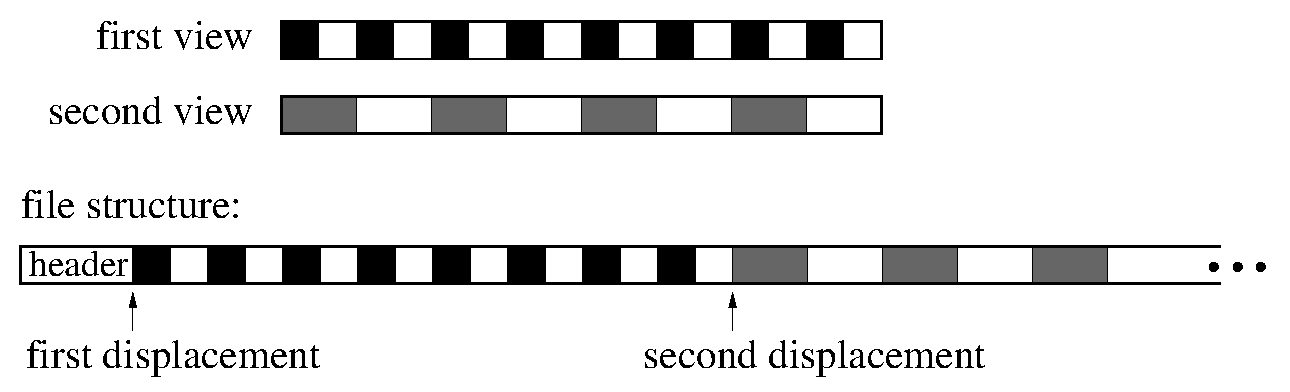
\includegraphics[width=4.0in]{figures/io-disp}}
  \caption{Displacements}
  \label{fig:io-disp}
\end{figure}
\end{users}

An \mpiterm{etype} (\mpitermni{elementary} datatype\mpitermindex{elementary datatype})
is the unit of data access and positioning.
It can be any \MPI/ predefined or derived datatype.
Derived etypes can be constructed
by using any of the \MPI/ datatype constructor routines,
provided all resulting typemap displacements are
nonnegative and monotonically increasing.
Data access is performed in etype units,
reading or writing whole data items of type etype.
Offsets are expressed as a count of etypes;
file pointers point to the beginning of etypes.

\begin{users}
In order to ensure interoperability in a heterogeneous environment,
additional restrictions must be observed when constructing the
\mpishortarg{etype}
(see \sectionref{sec:io-file-interop}).
\end{users}

A filetype is either a single etype or a derived \MPI/ datatype
constructed from multiple instances of the same etype.
In addition,
the extent of any hole in the filetype
must be a multiple of the etype's extent.
These displacements are not required to be distinct,
but they cannot be negative,
and they must be monotonically nondecreasing.

If the file is opened for writing,
neither the etype nor the filetype is permitted
to contain overlapping regions.
This restriction is equivalent to the ``datatype used in a receive
cannot specify overlapping regions'' restriction for communication.
Note that filetypes from different processes may still
overlap each other.

If a filetype has holes in it,
then the data in the holes is inaccessible to the calling process.
However, the \mpiarg{disp}, \mpiarg{etype}, and \mpiarg{filetype}
arguments can be changed via future calls to \mpifunc{MPI\_FILE\_SET\_VIEW}
to access a different part of the file.

It is erroneous to use absolute addresses in the construction
of the etype and filetype.

The \mpiarg{info} argument is used to provide information
regarding file access patterns and file system specifics
to direct optimization
(see \sectionref{sec:io-info}).
The constant \mpiconst{MPI\_INFO\_NULL} refers to the null info
and can be used when no info needs to be specified.

The \mpiarg{datarep} argument is a string that specifies
the representation of data in the file.
See the file interoperability section
(\sectionref{sec:io-file-interop})
for details and a discussion of valid values.

The user is responsible for ensuring that all nonblocking requests
and split collective operations
on \mpiarg{fh} have been completed before calling
\mpifunc{MPI\_FILE\_SET\_VIEW}---otherwise, the call to
\mpifunc{MPI\_FILE\_SET\_VIEW} is erroneous.

\cdeclindex{MPI\_File}%
\cdeclindex{MPI\_Offset}%
\begin{funcdef}{MPI\_FILE\_GET\_VIEW}{(\mbox{fh}, \mbox{disp}, \mbox{etype}, \mbox{filetype}, \mbox{datarep})}
\funcarg{\IN}{fh}{file handle (handle)}
\funcarg{\OUT}{disp}{displacement (integer)}
\funcarg{\OUT}{etype}{elementary datatype (handle)}
\funcarg{\OUT}{filetype}{filetype (handle)}
\funcarg{\OUT}{datarep}{data representation (string)}
\end{funcdef}
\mpibindmain{MPI\_File\_get\_view}{(\gb{}MPI\_File~fh, MPI\_Offset~*disp, MPI\_Datatype~*etype, MPI\_Datatype~*filetype, char~*datarep)}
\mpifnewbindmain{MPI\_File\_get\_view}{(fh, disp, etype, filetype, datarep, ierror) \fargs TYPE(MPI\_File), INTENT(IN)\ ::\ \mbox{fh}\fnarg{}INTEGER(KIND=MPI\_OFFSET\_KIND), INTENT(OUT)\ ::\ \mbox{disp}\fnarg{}TYPE(MPI\_Datatype), INTENT(OUT)\ ::\ \mbox{etype}, \mbox{filetype}\fnarg{}CHARACTER(LEN=*), INTENT(OUT)\ ::\ \mbox{datarep}\fnfinalarg{}INTEGER, OPTIONAL, INTENT(OUT)\ ::\ \mbox{ierror}}
\mpifbindmain{MPI\_FILE\_GET\_VIEW}{(FH, DISP, ETYPE, FILETYPE, DATAREP, IERROR) \fargs INTEGER \mbox{FH}, \mbox{ETYPE}, \mbox{FILETYPE}, \mbox{IERROR}\fnarg{}INTEGER(KIND=MPI\_OFFSET\_KIND) \mbox{DISP}\fnfinalarg{}CHARACTER*(*) \mbox{DATAREP}}

\mpifunc{MPI\_FILE\_GET\_VIEW} returns the process's view
of the data in the file.
The current value of the displacement is returned in \mpiarg{disp}.
The \mpiarg{etype} and \mpiarg{filetype} are new datatypes
with typemaps equal to the typemaps
of the current etype and filetype, respectively.

The data representation is returned in \mpiarg{datarep}.
The user is responsible for ensuring that \mpiarg{datarep} is
large enough to hold the returned data representation string.
The length of a data representation string is limited to the value of
\mpiconstmain{MPI\_MAX\_DATAREP\_STRING}.

In addition, if a portable datatype was used to set the current view,
then the corresponding datatype returned by \mpifunc{MPI\_FILE\_GET\_VIEW}
is also a portable datatype.
If \mpiarg{etype} or \mpiarg{filetype} are derived datatypes,
the user is responsible for freeing them.
The \mpiarg{etype} and \mpiarg{filetype} returned are both in a
committed state.

\section{Data Access}
\mpitermtitleindex{file!data access}
%====================
\label{sec:io-access}

\subsection{Data Access Routines}
%--------------------------------

Data is moved between files and processes by issuing read and write calls.
There are three orthogonal aspects to data access:
\mpitermdef{positioning} (explicit offset vs.\ implicit file pointer),
\mpitermdef{synchronism} (blocking vs.\ nonblocking and split collective),
and \mpitermdef{coordination} (noncollective vs.\ collective).
The following combinations of these data access routines,
including two types of file pointers (individual and shared)
are provided in Table~\ref{table:io:dataaccess}.

%
% This table doesn't fit on the page if merely small; footnotesize
% is required unless the table is reformatted.
\begin{table}[tb]
\caption{Data access routines}
\label{table:io:dataaccess}
\begin{center}
\footnotesize%%ALLOWLATEX%
\setlength{\tabcolsep}{1.75pt}%%ALLOWLATEX%% % to help fit in page width
\begin{tabular}{|l||l||l|l|}
\hline
\textbf{positioning} & \textbf{synchronism} & \multicolumn{2}{c|}{\textbf{coordination}} \\
\cline{3-4}
                &                 & noncollective   &
    collective\mpitermindex{collective} \\
\hline
\hline %-------------------------------------------------------------
explicit & \mpiterm{blocking}\mpitermindex{I/O!blocking}\mpitermindex{blocking I/O}%
  & \mpifunc{MPI\_FILE\_READ\_AT} & \mpifunc{MPI\_FILE\_READ\_AT\_ALL} \\
offsets & 
  & \mpifunc{MPI\_FILE\_WRITE\_AT} & \mpifunc{MPI\_FILE\_WRITE\_AT\_ALL} \\
\cline{2-4}
& \mpiterm{nonblocking}\mpitermindex{I/O!nonblocking}\mpitermindex{nonblocking I/O}%
  & \mpifunc{MPI\_FILE\_IREAD\_AT}  & \mpifunc{MPI\_FILE\_IREAD\_AT\_ALL} \\
& & \mpifunc{MPI\_FILE\_IWRITE\_AT} & \mpifunc{MPI\_FILE\_IWRITE\_AT\_ALL} \\
\cline{2-4}
& \mpiterm{split collective} & {N/A} & \mpifunc{MPI\_FILE\_READ\_AT\_ALL\_BEGIN} \\
& & & \mpifunc{MPI\_FILE\_READ\_AT\_ALL\_END} \\
& &                                  & \mpifunc{MPI\_FILE\_WRITE\_AT\_ALL\_BEGIN} \\
& &                                  & \mpifunc{MPI\_FILE\_WRITE\_AT\_ALL\_END} \\
\hline %-------------------------------------------------------------
individual    & \mpiterm{blocking}
  & \mpifunc{MPI\_FILE\_READ}   & \mpifunc{MPI\_FILE\_READ\_ALL} \\
file pointers &
  & \mpifunc{MPI\_FILE\_WRITE}  & \mpifunc{MPI\_FILE\_WRITE\_ALL} \\
\cline{2-4}
& \mpiterm{nonblocking}
  & \mpifunc{MPI\_FILE\_IREAD}  & \mpifunc{MPI\_FILE\_IREAD\_ALL} \\
& & \mpifunc{MPI\_FILE\_IWRITE} & \mpifunc{MPI\_FILE\_IWRITE\_ALL} \\
\cline{2-4}
& \mpiterm{split collective} & {N/A} & \mpifunc{MPI\_FILE\_READ\_ALL\_BEGIN} \\
& & & \mpifunc{MPI\_FILE\_READ\_ALL\_END} \\
& &                                  & \mpifunc{MPI\_FILE\_WRITE\_ALL\_BEGIN} \\
& &                                  & \mpifunc{MPI\_FILE\_WRITE\_ALL\_END} \\
\hline %-------------------------------------------------------------
shared       & \mpiterm{blocking}
  & \mpifunc{MPI\_FILE\_READ\_SHARED}   & \mpifunc{MPI\_FILE\_READ\_ORDERED} \\
file pointer &
  & \mpifunc{MPI\_FILE\_WRITE\_SHARED}  & \mpifunc{MPI\_FILE\_WRITE\_ORDERED} \\
\cline{2-4}
& \mpiterm{nonblocking}
  & \mpifunc{MPI\_FILE\_IREAD\_SHARED}  & {N/A} \\
& & \mpifunc{MPI\_FILE\_IWRITE\_SHARED} & \\
\cline{2-4}
& \mpiterm{split collective} & {N/A} & \mpifunc{MPI\_FILE\_READ\_ORDERED\_BEGIN} \\
& & & \mpifunc{MPI\_FILE\_READ\_ORDERED\_END} \\
& &                                  & \mpifunc{MPI\_FILE\_WRITE\_ORDERED\_BEGIN} \\
& &                                  & \mpifunc{MPI\_FILE\_WRITE\_ORDERED\_END} \\
\hline
\end{tabular}
\end{center}
\end{table} 

POSIX \code{read()}/\code{fread()} and \code{write()}/\code{fwrite()} are blocking,
noncollective operations and use individual file pointers\mpitermindex{POSIX!I/O}.
The \MPI/ counterparts are \mpifunc{MPI\_FILE\_READ} and \mpifunc{MPI\_FILE\_WRITE}.

Implementations of data access routines may buffer data to improve
performance.  This does not affect reads, as the data is always
available in the user's buffer after a read operation completes.
For writes, however, the \mpifunc{MPI\_FILE\_SYNC} routine provides the only
guarantee that data has been transferred to the storage device.

\subsubsection{Positioning}
%--------------------------

\MPI/ provides three types of positioning for data access routines:
\mpitermdef{explicit offsets}, \mpitermdef{individual file pointers}, and \mpitermdef{shared file pointers}.
The different positioning methods may be mixed within the same program
and do not affect each other.

The data access routines that accept explicit offsets
contain \mpicode{\_AT}
in their name (e.g., \mpifunc{MPI\_FILE\_WRITE\_AT}).
Explicit offset operations perform data access at
the file position given directly as an argument---no
file pointer is used nor updated.
Note that this is not equivalent to an atomic seek-and-read
or seek-and-write operation,
as no ``seek'' is issued.
Operations with explicit offsets are described in
\sectionref{sec:io-explicit}.

The names of the individual file pointer routines contain no
positional qualifier (e.g., \mpifunc{MPI\_FILE\_WRITE}).
Operations with individual file pointers are described in
\sectionref{sec:io-indiv-ptr}.
The data access routines that use shared file pointers contain
\mpicode{\_SHARED} 
or \mpicode{\_ORDERED} 
in their name (e.g., \mpifunc{MPI\_FILE\_WRITE\_SHARED}).
Operations with shared file pointers are described in
\sectionref{sec:io-shared-ptr}.

The main semantic issues with \MPI/-maintained file pointers
are how and when they are updated by I/O operations.
In general, each I/O operation leaves the file pointer pointing to the
next data item after the last one that
is accessed by the operation.
In a nonblocking or split collective operation,
the pointer is updated by the call that initiates the I/O,
possibly before the access completes.

% Must use \textit here to have ff typeset as a ligature. Otherwise, this
% text is ugly. Using %ALLOWLATEX% to permit use here.
More formally,
\[
    \textit{new\_file\_offset} = \textit{old\_file\_offset} + %ALLOWLATEX%
                \frac{elements(datatype)}{elements(etype)} \times count
\]
where $count$ is the number of $datatype$ items to be accessed,
$elements(X)$ is the number of predefined datatypes in the typemap of $X$,
and \textit{old\_file\_offset} is %ALLOWLATEX%
the value of the implicit offset before the call.
The file position, \textit{new\_file\_offset}, is in terms %ALLOWLATEX%
of a count of etypes relative to the current view.

\subsubsection{Synchronism}
%--------------------------

\MPI/ supports blocking and nonblocking I/O routines.

A \mpitermni{blocking}\mpitermindex{blocking!I/O} I/O call will
not return
until the I/O request is completed.

A \mpitermni{nonblocking}\mpitermindex{nonblocking!I/O} I/O call initiates an I/O operation, but does not
wait for it to complete.  Given suitable hardware, this allows the
transfer of data out of and into the user's buffer to proceed concurrently with
computation.  A separate \mpitermni{request complete}\mpitermindex{request complete!I/O} call
(\mpifunc{MPI\_WAIT}, \mpifunc{MPI\_TEST}, or any of their variants) is
needed to complete the I/O request,
i.e., to confirm that the data has been read or written and that
it is safe for the user to reuse the buffer.
The nonblocking versions of the routines are named
\mpicode{MPI\_FILE\_I\XXX/}, where the \mpicode{I} stands for immediate.

It is erroneous to access the local buffer of a nonblocking
data access operation, or to use that buffer as the source or
target of other communications, between the initiation and
completion of the operation. 

The split collective routines
support a restricted form of ``nonblocking'' operations
for collective data access
(see \sectionref{sec:io-split-collective}).

\subsubsection{Coordination}
%------------------------

Every noncollective data access routine \mpicode{MPI\_FILE\_\XXX/}
has a collective counterpart.  For most routines, this counterpart
is \mpicode{MPI\_FILE\_\XXX/\_ALL} or a pair of 
\mpicode{MPI\_FILE\_\XXX/\_BEGIN} and 
\mpicode{MPI\_FILE\_\XXX/\_END}.
The counterparts to the \mpicode{MPI\_FILE\_\XXX/\_SHARED} routines are 
\mpicode{MPI\_FILE\_\XXX/\_ORDERED}.

The completion of a noncollective call only depends on the activity of
the calling process.
However, the completion of a collective call
(which must be called by all members of the process group)
may depend on the activity
of the other processes participating in the collective call.
See \sectionref{sec:io-semantics-collective}
for rules on semantics of collective calls.

Collective operations
may perform much better than their noncollective counterparts,
as global data accesses have significant potential for automatic optimization.

\subsubsection{Data Access Conventions}
%- - - - - - - - - - - - - - - - - - -
\label{sec:io-data-access-conventions}

Data is moved between files and processes
by calling read and write routines.
Read routines move data from a file into memory.
Write routines move data from memory into a file.
The file is designated by a file handle, \mpiarg{fh}.
The location of the file data is specified by an offset
into the current view.
The data in memory is specified by a triple:
\mpiarg{buf}, \mpiarg{count}, and \mpiarg{datatype}.
Upon completion, the amount of data accessed
by the calling process is returned in a \mpiarg{status}.

An offset designates the starting position in the file for an access.
The offset is always in etype units relative to the current view.
Explicit offset routines pass \mpiarg{offset} as an argument
(negative values are erroneous).
The file pointer routines use implicit offsets maintained by \MPI/.

A data access routine attempts to transfer (read or write)
\mpiarg{count} data items
of type \mpiarg{datatype} between the user's buffer \mpiarg{buf}
and the file.
The \mpiarg{datatype} passed to the routine must be 
a committed datatype.
The layout of data in memory corresponding to
\mpiarg{buf}, \mpiarg{count}, \mpiarg{datatype} is
interpreted the same way as in 
\MPI/ 
communication functions;
see \sectionref{subsec:pt2pt-messagedata} and 
\sectionref{subsec:pt2pt-datatypeuse}. 
The data is accessed
from those parts of the file specified by the current view
(\sectionref{sec:io-view}).
The type signature of \mpiarg{datatype} must match
the type signature of some number of contiguous copies of the \mpiarg{etype}
of the current view.
As in a receive,
it is erroneous to specify a \mpiarg{datatype}
for reading that contains overlapping regions
(areas of memory that would be stored into more than once).

The nonblocking data access routines
indicate that \MPI/ can start a data access
and associate a request handle, \mpiarg{request},
with the I/O 
operation.
Nonblocking operations are completed via
\mpifunc{MPI\_TEST}, \mpifunc{MPI\_WAIT}, or any of their variants.

Data access operations, when completed,
return the amount of data accessed in \mpiarg{status}.

%% See comments in pt2pt.tex on why the commented out part is both 
%% unnecessary and incorrect.
\begin{users}
To prevent problems with the argument copying and register
optimization done by Fortran compilers, please note the hints in
%
Sections~\ref{sec:misc-problems}--\ref{sec:f90-problems:comparison-with-C}.
%% especially in 
%% %
%% Sections~\ref{sec:misc-sequence} and~\ref{sec:f90-problems:vector-subscripts}
%% on pages~\pageref{sec:misc-sequence}--\pageref{sec:f90-problems:vector-subscripts}
%% about ``Problems Due to Data Copying and Sequence Association with Subscript Triplets''
%% and ``Vector Subscripts,''
%% and in Sections~\ref{sec:misc-register} to~\ref{sec:f90-problems:perm-data-movements}
%% on pages~\pageref{sec:misc-register} to~\pageref{sec:f90-problems:perm-data-movements} 
%% about ``Optimization Problems,'' ``Code Movements and Register Optimization,''
%% ``Temporary Data Movements,'' and ``Permanent Data Movements.''
\end{users}

For blocking routines, \mpiarg{status} is returned directly.
For nonblocking routines and split collective routines,
\mpiarg{status} is returned when the operation is completed.
The number of \mpiarg{datatype} entries and predefined elements accessed
by the calling process
can be extracted from \mpiarg{status} by using
\mpifunc{MPI\_GET\_COUNT} and
\mpifunc{MPI\_GET\_ELEMENTS}, respectively.
The interpretation of the \mpicode{MPI\_ERROR} field is the same as for other
operations---normally undefined, but meaningful if an \MPI/ routine returns 
\error{MPI\_ERR\_IN\_STATUS}.
The user can pass (in C and
Fortran)
\mpiconst{MPI\_STATUS\_IGNORE}
in the \mpiarg{status} argument
if the return value of this argument is not needed.
The \mpiarg{status} can be passed to \mpifunc{MPI\_TEST\_CANCELLED}
to determine if the operation was cancelled.
All other fields of \mpiarg{status} are undefined.

When reading, a program can detect the end of the file
by noting that the amount of data read is less than the amount requested.
Writing past the end of the file increases the file size.
The amount of data accessed will be the amount requested,
unless an error is raised (or a read reaches the end of the file).

\subsection{Data Access with Explicit Offsets}
\mpitermtitleindex{explicit offsets}
\mpitermtitleindex{file!data access!explicit offsets}
\mpitermtitleindex{semantics!file!explicit offsets}
%---------------------------------------------
\label{sec:io-explicit}

If \mpiconst{MPI\_MODE\_SEQUENTIAL} mode was specified when the file was opened,
it is erroneous to call the routines in this section.

\cdeclindex{MPI\_File}%
\cdeclindex{MPI\_Status}%
\cdeclindex{MPI\_Offset}%
\begin{funcdef}{MPI\_FILE\_READ\_AT}{(\mbox{fh}, \mbox{offset}, \mbox{buf}, \mbox{count}, \mbox{datatype}, \mbox{status})}
\funcarg{\IN}{fh}{file handle (handle)}
\funcarg{\IN}{offset}{file offset (integer)}
\funcarg{\OUT}{buf}{initial address of buffer (choice)}
\funcarg{\IN}{count}{number of elements in buffer (integer)}
\funcarg{\IN}{datatype}{datatype of each buffer element (handle)}
\funcarg{\OUT}{status}{status object (status)}
\end{funcdef}
\mpibindmain{MPI\_File\_read\_at}{(\gb{}MPI\_File~fh, MPI\_Offset~offset, void~*buf, int~count, MPI\_Datatype~datatype, MPI\_Status~*status)}
\MPIbindindex{MPI\_File\_read\_at\_c}
\mpibindmain{MPI\_File\_read\_at\_c}{(\gb{}MPI\_File~fh, MPI\_Offset~offset, void~*buf, MPI\_Count~count, MPI\_Datatype~datatype, MPI\_Status~*status)}
\mpifnewbindmain{MPI\_File\_read\_at}{(fh, offset, buf, count, datatype, status, ierror) \fargs TYPE(MPI\_File), INTENT(IN)\ ::\ \mbox{fh}\fnarg{}INTEGER(KIND=MPI\_OFFSET\_KIND), INTENT(IN)\ ::\ \mbox{offset}\fnarg{}TYPE(*), DIMENSION(..)\ ::\ \mbox{buf}\fnarg{}INTEGER, INTENT(IN)\ ::\ \mbox{count}\fnarg{}TYPE(MPI\_Datatype), INTENT(IN)\ ::\ \mbox{datatype}\fnarg{}TYPE(MPI\_Status)\ ::\ \mbox{status}\fnfinalarg{}INTEGER, OPTIONAL, INTENT(OUT)\ ::\ \mbox{ierror}}
\mpifnewbindmain{MPI\_File\_read\_at}{(fh, offset, buf, count, datatype, status, ierror) !(\_c) \fargs TYPE(MPI\_File), INTENT(IN)\ ::\ \mbox{fh}\fnarg{}INTEGER(KIND=MPI\_OFFSET\_KIND), INTENT(IN)\ ::\ \mbox{offset}\fnarg{}TYPE(*), DIMENSION(..)\ ::\ \mbox{buf}\fnarg{}INTEGER(KIND=MPI\_COUNT\_KIND), INTENT(IN)\ ::\ \mbox{count}\fnarg{}TYPE(MPI\_Datatype), INTENT(IN)\ ::\ \mbox{datatype}\fnarg{}TYPE(MPI\_Status)\ ::\ \mbox{status}\fnfinalarg{}INTEGER, OPTIONAL, INTENT(OUT)\ ::\ \mbox{ierror}}
\mpifbindmain{MPI\_FILE\_READ\_AT}{(FH, OFFSET, BUF, COUNT, DATATYPE, STATUS, IERROR) \fargs INTEGER \mbox{FH}, \mbox{COUNT}, \mbox{DATATYPE}, \mbox{STATUS(MPI\_STATUS\_SIZE)}, \mbox{IERROR}\fnarg{}INTEGER(KIND=MPI\_OFFSET\_KIND) \mbox{OFFSET}\fnfinalarg{}<type> \mbox{BUF(*)}}

\mpifunc{MPI\_FILE\_READ\_AT} reads a file
beginning at the position specified by \mpiarg{offset}.

\cdeclindex{MPI\_File}%
\cdeclindex{MPI\_Status}%
\cdeclindex{MPI\_Offset}%
\begin{funcdef}{MPI\_FILE\_READ\_AT\_ALL}{(\mbox{fh}, \mbox{offset}, \mbox{buf}, \mbox{count}, \mbox{datatype}, \mbox{status})}
\funcarg{\IN}{fh}{file handle (handle)}
\funcarg{\IN}{offset}{file offset (integer)}
\funcarg{\OUT}{buf}{initial address of buffer (choice)}
\funcarg{\IN}{count}{number of elements in buffer (integer)}
\funcarg{\IN}{datatype}{datatype of each buffer element (handle)}
\funcarg{\OUT}{status}{status object (status)}
\end{funcdef}
\mpibindmain{MPI\_File\_read\_at\_all}{(\gb{}MPI\_File~fh, MPI\_Offset~offset, void~*buf, int~count, MPI\_Datatype~datatype, MPI\_Status~*status)}
\MPIbindindex{MPI\_File\_read\_at\_all\_c}
\mpibindmain{MPI\_File\_read\_at\_all\_c}{(\gb{}MPI\_File~fh, MPI\_Offset~offset, void~*buf, MPI\_Count~count, MPI\_Datatype~datatype, MPI\_Status~*status)}
\mpifnewbindmain{MPI\_File\_read\_at\_all}{(fh, offset, buf, count, datatype, status, ierror) \fargs TYPE(MPI\_File), INTENT(IN)\ ::\ \mbox{fh}\fnarg{}INTEGER(KIND=MPI\_OFFSET\_KIND), INTENT(IN)\ ::\ \mbox{offset}\fnarg{}TYPE(*), DIMENSION(..)\ ::\ \mbox{buf}\fnarg{}INTEGER, INTENT(IN)\ ::\ \mbox{count}\fnarg{}TYPE(MPI\_Datatype), INTENT(IN)\ ::\ \mbox{datatype}\fnarg{}TYPE(MPI\_Status)\ ::\ \mbox{status}\fnfinalarg{}INTEGER, OPTIONAL, INTENT(OUT)\ ::\ \mbox{ierror}}
\mpifnewbindmain{MPI\_File\_read\_at\_all}{(fh, offset, buf, count, datatype, status, ierror) !(\_c) \fargs TYPE(MPI\_File), INTENT(IN)\ ::\ \mbox{fh}\fnarg{}INTEGER(KIND=MPI\_OFFSET\_KIND), INTENT(IN)\ ::\ \mbox{offset}\fnarg{}TYPE(*), DIMENSION(..)\ ::\ \mbox{buf}\fnarg{}INTEGER(KIND=MPI\_COUNT\_KIND), INTENT(IN)\ ::\ \mbox{count}\fnarg{}TYPE(MPI\_Datatype), INTENT(IN)\ ::\ \mbox{datatype}\fnarg{}TYPE(MPI\_Status)\ ::\ \mbox{status}\fnfinalarg{}INTEGER, OPTIONAL, INTENT(OUT)\ ::\ \mbox{ierror}}
\mpifbindmain{MPI\_FILE\_READ\_AT\_ALL}{(FH, OFFSET, BUF, COUNT, DATATYPE, STATUS, IERROR) \fargs INTEGER \mbox{FH}, \mbox{COUNT}, \mbox{DATATYPE}, \mbox{STATUS(MPI\_STATUS\_SIZE)}, \mbox{IERROR}\fnarg{}INTEGER(KIND=MPI\_OFFSET\_KIND) \mbox{OFFSET}\fnfinalarg{}<type> \mbox{BUF(*)}}

\mpifunc{MPI\_FILE\_READ\_AT\_ALL} is a collective version
of the blocking \mpifunc{MPI\_FILE\_READ\_AT} interface.

\cdeclindex{MPI\_File}%
\cdeclindex{MPI\_Status}%
\cdeclindex{MPI\_Offset}%
\begin{funcdef}{MPI\_FILE\_WRITE\_AT}{(\mbox{fh}, \mbox{offset}, \mbox{buf}, \mbox{count}, \mbox{datatype}, \mbox{status})}
\funcarg{\INOUT}{fh}{file handle (handle)}
\funcarg{\IN}{offset}{file offset (integer)}
\funcarg{\IN}{buf}{initial address of buffer (choice)}
\funcarg{\IN}{count}{number of elements in buffer (integer)}
\funcarg{\IN}{datatype}{datatype of each buffer element (handle)}
\funcarg{\OUT}{status}{status object (status)}
\end{funcdef}
\mpibindmain{MPI\_File\_write\_at}{(\gb{}MPI\_File~fh, MPI\_Offset~offset, const~void~*buf, int~count, MPI\_Datatype~datatype, MPI\_Status~*status)}
\MPIbindindex{MPI\_File\_write\_at\_c}
\mpibindmain{MPI\_File\_write\_at\_c}{(\gb{}MPI\_File~fh, MPI\_Offset~offset, const~void~*buf, MPI\_Count~count, MPI\_Datatype~datatype, MPI\_Status~*status)}
\mpifnewbindmain{MPI\_File\_write\_at}{(fh, offset, buf, count, datatype, status, ierror) \fargs TYPE(MPI\_File), INTENT(IN)\ ::\ \mbox{fh}\fnarg{}INTEGER(KIND=MPI\_OFFSET\_KIND), INTENT(IN)\ ::\ \mbox{offset}\fnarg{}TYPE(*), DIMENSION(..), INTENT(IN)\ ::\ \mbox{buf}\fnarg{}INTEGER, INTENT(IN)\ ::\ \mbox{count}\fnarg{}TYPE(MPI\_Datatype), INTENT(IN)\ ::\ \mbox{datatype}\fnarg{}TYPE(MPI\_Status)\ ::\ \mbox{status}\fnfinalarg{}INTEGER, OPTIONAL, INTENT(OUT)\ ::\ \mbox{ierror}}
\mpifnewbindmain{MPI\_File\_write\_at}{(fh, offset, buf, count, datatype, status, ierror) !(\_c) \fargs TYPE(MPI\_File), INTENT(IN)\ ::\ \mbox{fh}\fnarg{}INTEGER(KIND=MPI\_OFFSET\_KIND), INTENT(IN)\ ::\ \mbox{offset}\fnarg{}TYPE(*), DIMENSION(..), INTENT(IN)\ ::\ \mbox{buf}\fnarg{}INTEGER(KIND=MPI\_COUNT\_KIND), INTENT(IN)\ ::\ \mbox{count}\fnarg{}TYPE(MPI\_Datatype), INTENT(IN)\ ::\ \mbox{datatype}\fnarg{}TYPE(MPI\_Status)\ ::\ \mbox{status}\fnfinalarg{}INTEGER, OPTIONAL, INTENT(OUT)\ ::\ \mbox{ierror}}
\mpifbindmain{MPI\_FILE\_WRITE\_AT}{(FH, OFFSET, BUF, COUNT, DATATYPE, STATUS, IERROR) \fargs INTEGER \mbox{FH}, \mbox{COUNT}, \mbox{DATATYPE}, \mbox{STATUS(MPI\_STATUS\_SIZE)}, \mbox{IERROR}\fnarg{}INTEGER(KIND=MPI\_OFFSET\_KIND) \mbox{OFFSET}\fnfinalarg{}<type> \mbox{BUF(*)}}

\mpifunc{MPI\_FILE\_WRITE\_AT} writes a file
beginning at the position specified by \mpiarg{offset}.


\cdeclindex{MPI\_File}%
\cdeclindex{MPI\_Status}%
\cdeclindex{MPI\_Offset}%
\begin{funcdef}{MPI\_FILE\_WRITE\_AT\_ALL}{(\mbox{fh}, \mbox{offset}, \mbox{buf}, \mbox{count}, \mbox{datatype}, \mbox{status})}
\funcarg{\INOUT}{fh}{file handle (handle)}
\funcarg{\IN}{offset}{file offset (integer)}
\funcarg{\IN}{buf}{initial address of buffer (choice)}
\funcarg{\IN}{count}{number of elements in buffer (integer)}
\funcarg{\IN}{datatype}{datatype of each buffer element (handle)}
\funcarg{\OUT}{status}{status object (status)}
\end{funcdef}
\mpibindmain{MPI\_File\_write\_at\_all}{(\gb{}MPI\_File~fh, MPI\_Offset~offset, const~void~*buf, int~count, MPI\_Datatype~datatype, MPI\_Status~*status)}
\MPIbindindex{MPI\_File\_write\_at\_all\_c}
\mpibindmain{MPI\_File\_write\_at\_all\_c}{(\gb{}MPI\_File~fh, MPI\_Offset~offset, const~void~*buf, MPI\_Count~count, MPI\_Datatype~datatype, MPI\_Status~*status)}
\mpifnewbindmain{MPI\_File\_write\_at\_all}{(fh, offset, buf, count, datatype, status, ierror) \fargs TYPE(MPI\_File), INTENT(IN)\ ::\ \mbox{fh}\fnarg{}INTEGER(KIND=MPI\_OFFSET\_KIND), INTENT(IN)\ ::\ \mbox{offset}\fnarg{}TYPE(*), DIMENSION(..), INTENT(IN)\ ::\ \mbox{buf}\fnarg{}INTEGER, INTENT(IN)\ ::\ \mbox{count}\fnarg{}TYPE(MPI\_Datatype), INTENT(IN)\ ::\ \mbox{datatype}\fnarg{}TYPE(MPI\_Status)\ ::\ \mbox{status}\fnfinalarg{}INTEGER, OPTIONAL, INTENT(OUT)\ ::\ \mbox{ierror}}
\mpifnewbindmain{MPI\_File\_write\_at\_all}{(fh, offset, buf, count, datatype, status, ierror) !(\_c) \fargs TYPE(MPI\_File), INTENT(IN)\ ::\ \mbox{fh}\fnarg{}INTEGER(KIND=MPI\_OFFSET\_KIND), INTENT(IN)\ ::\ \mbox{offset}\fnarg{}TYPE(*), DIMENSION(..), INTENT(IN)\ ::\ \mbox{buf}\fnarg{}INTEGER(KIND=MPI\_COUNT\_KIND), INTENT(IN)\ ::\ \mbox{count}\fnarg{}TYPE(MPI\_Datatype), INTENT(IN)\ ::\ \mbox{datatype}\fnarg{}TYPE(MPI\_Status)\ ::\ \mbox{status}\fnfinalarg{}INTEGER, OPTIONAL, INTENT(OUT)\ ::\ \mbox{ierror}}
\mpifbindmain{MPI\_FILE\_WRITE\_AT\_ALL}{(FH, OFFSET, BUF, COUNT, DATATYPE, STATUS, IERROR) \fargs INTEGER \mbox{FH}, \mbox{COUNT}, \mbox{DATATYPE}, \mbox{STATUS(MPI\_STATUS\_SIZE)}, \mbox{IERROR}\fnarg{}INTEGER(KIND=MPI\_OFFSET\_KIND) \mbox{OFFSET}\fnfinalarg{}<type> \mbox{BUF(*)}}

\mpifunc{MPI\_FILE\_WRITE\_AT\_ALL} is a collective version
of the blocking \mpifunc{MPI\_FILE\_WRITE\_AT} interface.

\cdeclindex{MPI\_Request}%
\cdeclindex{MPI\_File}%
\cdeclindex{MPI\_Offset}%
\begin{funcdef}{MPI\_FILE\_IREAD\_AT}{(\mbox{fh}, \mbox{offset}, \mbox{buf}, \mbox{count}, \mbox{datatype}, \mbox{request})}
\funcarg{\IN}{fh}{file handle (handle)}
\funcarg{\IN}{offset}{file offset (integer)}
\funcarg{\OUT}{buf}{initial address of buffer (choice)}
\funcarg{\IN}{count}{number of elements in buffer (integer)}
\funcarg{\IN}{datatype}{datatype of each buffer element (handle)}
\funcarg{\OUT}{request}{request object (handle)}
\end{funcdef}
\mpibindmain{MPI\_File\_iread\_at}{(\gb{}MPI\_File~fh, MPI\_Offset~offset, void~*buf, int~count, MPI\_Datatype~datatype, MPI\_Request~*request)}
\MPIbindindex{MPI\_File\_iread\_at\_c}
\mpibindmain{MPI\_File\_iread\_at\_c}{(\gb{}MPI\_File~fh, MPI\_Offset~offset, void~*buf, MPI\_Count~count, MPI\_Datatype~datatype, MPI\_Request~*request)}
\mpifnewbindmain{MPI\_File\_iread\_at}{(fh, offset, buf, count, datatype, request, ierror) \fargs TYPE(MPI\_File), INTENT(IN)\ ::\ \mbox{fh}\fnarg{}INTEGER(KIND=MPI\_OFFSET\_KIND), INTENT(IN)\ ::\ \mbox{offset}\fnarg{}TYPE(*), DIMENSION(..), ASYNCHRONOUS\ ::\ \mbox{buf}\fnarg{}INTEGER, INTENT(IN)\ ::\ \mbox{count}\fnarg{}TYPE(MPI\_Datatype), INTENT(IN)\ ::\ \mbox{datatype}\fnarg{}TYPE(MPI\_Request), INTENT(OUT)\ ::\ \mbox{request}\fnfinalarg{}INTEGER, OPTIONAL, INTENT(OUT)\ ::\ \mbox{ierror}}
\mpifnewbindmain{MPI\_File\_iread\_at}{(fh, offset, buf, count, datatype, request, ierror) !(\_c) \fargs TYPE(MPI\_File), INTENT(IN)\ ::\ \mbox{fh}\fnarg{}INTEGER(KIND=MPI\_OFFSET\_KIND), INTENT(IN)\ ::\ \mbox{offset}\fnarg{}TYPE(*), DIMENSION(..), ASYNCHRONOUS\ ::\ \mbox{buf}\fnarg{}INTEGER(KIND=MPI\_COUNT\_KIND), INTENT(IN)\ ::\ \mbox{count}\fnarg{}TYPE(MPI\_Datatype), INTENT(IN)\ ::\ \mbox{datatype}\fnarg{}TYPE(MPI\_Request), INTENT(OUT)\ ::\ \mbox{request}\fnfinalarg{}INTEGER, OPTIONAL, INTENT(OUT)\ ::\ \mbox{ierror}}
\mpifbindmain{MPI\_FILE\_IREAD\_AT}{(FH, OFFSET, BUF, COUNT, DATATYPE, REQUEST, IERROR) \fargs INTEGER \mbox{FH}, \mbox{COUNT}, \mbox{DATATYPE}, \mbox{REQUEST}, \mbox{IERROR}\fnarg{}INTEGER(KIND=MPI\_OFFSET\_KIND) \mbox{OFFSET}\fnfinalarg{}<type> \mbox{BUF(*)}}

\mpifunc{MPI\_FILE\_IREAD\_AT} is a nonblocking version
of the \mpifunc{MPI\_FILE\_READ\_AT} interface.

\cdeclindex{MPI\_Request}%
\cdeclindex{MPI\_File}%
\cdeclindex{MPI\_Offset}%
\begin{funcdef}{MPI\_FILE\_IREAD\_AT\_ALL}{(\mbox{fh}, \mbox{offset}, \mbox{buf}, \mbox{count}, \mbox{datatype}, \mbox{request})}
\funcarg{\IN}{fh}{file handle (handle)}
\funcarg{\IN}{offset}{file offset (integer)}
\funcarg{\OUT}{buf}{initial address of buffer (choice)}
\funcarg{\IN}{count}{number of elements in buffer (integer)}
\funcarg{\IN}{datatype}{datatype of each buffer element (handle)}
\funcarg{\OUT}{request}{request object (handle)}
\end{funcdef}
\mpibindmain{MPI\_File\_iread\_at\_all}{(\gb{}MPI\_File~fh, MPI\_Offset~offset, void~*buf, int~count, MPI\_Datatype~datatype, MPI\_Request~*request)}
\MPIbindindex{MPI\_File\_iread\_at\_all\_c}
\mpibindmain{MPI\_File\_iread\_at\_all\_c}{(\gb{}MPI\_File~fh, MPI\_Offset~offset, void~*buf, MPI\_Count~count, MPI\_Datatype~datatype, MPI\_Request~*request)}
\mpifnewbindmain{MPI\_File\_iread\_at\_all}{(fh, offset, buf, count, datatype, request, ierror) \fargs TYPE(MPI\_File), INTENT(IN)\ ::\ \mbox{fh}\fnarg{}INTEGER(KIND=MPI\_OFFSET\_KIND), INTENT(IN)\ ::\ \mbox{offset}\fnarg{}TYPE(*), DIMENSION(..), ASYNCHRONOUS\ ::\ \mbox{buf}\fnarg{}INTEGER, INTENT(IN)\ ::\ \mbox{count}\fnarg{}TYPE(MPI\_Datatype), INTENT(IN)\ ::\ \mbox{datatype}\fnarg{}TYPE(MPI\_Request), INTENT(OUT)\ ::\ \mbox{request}\fnfinalarg{}INTEGER, OPTIONAL, INTENT(OUT)\ ::\ \mbox{ierror}}
\mpifnewbindmain{MPI\_File\_iread\_at\_all}{(fh, offset, buf, count, datatype, request, ierror) !(\_c) \fargs TYPE(MPI\_File), INTENT(IN)\ ::\ \mbox{fh}\fnarg{}INTEGER(KIND=MPI\_OFFSET\_KIND), INTENT(IN)\ ::\ \mbox{offset}\fnarg{}TYPE(*), DIMENSION(..), ASYNCHRONOUS\ ::\ \mbox{buf}\fnarg{}INTEGER(KIND=MPI\_COUNT\_KIND), INTENT(IN)\ ::\ \mbox{count}\fnarg{}TYPE(MPI\_Datatype), INTENT(IN)\ ::\ \mbox{datatype}\fnarg{}TYPE(MPI\_Request), INTENT(OUT)\ ::\ \mbox{request}\fnfinalarg{}INTEGER, OPTIONAL, INTENT(OUT)\ ::\ \mbox{ierror}}
\mpifbindmain{MPI\_FILE\_IREAD\_AT\_ALL}{(FH, OFFSET, BUF, COUNT, DATATYPE, REQUEST, IERROR) \fargs INTEGER \mbox{FH}, \mbox{COUNT}, \mbox{DATATYPE}, \mbox{REQUEST}, \mbox{IERROR}\fnarg{}INTEGER(KIND=MPI\_OFFSET\_KIND) \mbox{OFFSET}\fnfinalarg{}<type> \mbox{BUF(*)}}

\mpifunc{MPI\_FILE\_IREAD\_AT\_ALL} is a nonblocking version of
\mpifunc{MPI\_FILE\_READ\_AT\_ALL}. See
\sectionref{sec:io-semantics-nb-collective}
for semantics of nonblocking
collective file operations.

\cdeclindex{MPI\_Request}%
\cdeclindex{MPI\_File}%
\cdeclindex{MPI\_Offset}%
\begin{funcdef}{MPI\_FILE\_IWRITE\_AT}{(\mbox{fh}, \mbox{offset}, \mbox{buf}, \mbox{count}, \mbox{datatype}, \mbox{request})}
\funcarg{\INOUT}{fh}{file handle (handle)}
\funcarg{\IN}{offset}{file offset (integer)}
\funcarg{\IN}{buf}{initial address of buffer (choice)}
\funcarg{\IN}{count}{number of elements in buffer (integer)}
\funcarg{\IN}{datatype}{datatype of each buffer element (handle)}
\funcarg{\OUT}{request}{request object (handle)}
\end{funcdef}
\mpibindmain{MPI\_File\_iwrite\_at}{(\gb{}MPI\_File~fh, MPI\_Offset~offset, const~void~*buf, int~count, MPI\_Datatype~datatype, MPI\_Request~*request)}
\MPIbindindex{MPI\_File\_iwrite\_at\_c}
\mpibindmain{MPI\_File\_iwrite\_at\_c}{(\gb{}MPI\_File~fh, MPI\_Offset~offset, const~void~*buf, MPI\_Count~count, MPI\_Datatype~datatype, MPI\_Request~*request)}
\mpifnewbindmain{MPI\_File\_iwrite\_at}{(fh, offset, buf, count, datatype, request, ierror) \fargs TYPE(MPI\_File), INTENT(IN)\ ::\ \mbox{fh}\fnarg{}INTEGER(KIND=MPI\_OFFSET\_KIND), INTENT(IN)\ ::\ \mbox{offset}\fnarg{}TYPE(*), DIMENSION(..), INTENT(IN), ASYNCHRONOUS\ ::\ \mbox{buf}\fnarg{}INTEGER, INTENT(IN)\ ::\ \mbox{count}\fnarg{}TYPE(MPI\_Datatype), INTENT(IN)\ ::\ \mbox{datatype}\fnarg{}TYPE(MPI\_Request), INTENT(OUT)\ ::\ \mbox{request}\fnfinalarg{}INTEGER, OPTIONAL, INTENT(OUT)\ ::\ \mbox{ierror}}
\mpifnewbindmain{MPI\_File\_iwrite\_at}{(fh, offset, buf, count, datatype, request, ierror) !(\_c) \fargs TYPE(MPI\_File), INTENT(IN)\ ::\ \mbox{fh}\fnarg{}INTEGER(KIND=MPI\_OFFSET\_KIND), INTENT(IN)\ ::\ \mbox{offset}\fnarg{}TYPE(*), DIMENSION(..), INTENT(IN), ASYNCHRONOUS\ ::\ \mbox{buf}\fnarg{}INTEGER(KIND=MPI\_COUNT\_KIND), INTENT(IN)\ ::\ \mbox{count}\fnarg{}TYPE(MPI\_Datatype), INTENT(IN)\ ::\ \mbox{datatype}\fnarg{}TYPE(MPI\_Request), INTENT(OUT)\ ::\ \mbox{request}\fnfinalarg{}INTEGER, OPTIONAL, INTENT(OUT)\ ::\ \mbox{ierror}}
\mpifbindmain{MPI\_FILE\_IWRITE\_AT}{(FH, OFFSET, BUF, COUNT, DATATYPE, REQUEST, IERROR) \fargs INTEGER \mbox{FH}, \mbox{COUNT}, \mbox{DATATYPE}, \mbox{REQUEST}, \mbox{IERROR}\fnarg{}INTEGER(KIND=MPI\_OFFSET\_KIND) \mbox{OFFSET}\fnfinalarg{}<type> \mbox{BUF(*)}}

\mpifunc{MPI\_FILE\_IWRITE\_AT} is a nonblocking version
of the \mpifunc{MPI\_FILE\_WRITE\_AT} interface.

\cdeclindex{MPI\_Request}%
\cdeclindex{MPI\_File}%
\cdeclindex{MPI\_Offset}%
\begin{funcdef}{MPI\_FILE\_IWRITE\_AT\_ALL}{(\mbox{fh}, \mbox{offset}, \mbox{buf}, \mbox{count}, \mbox{datatype}, \mbox{request})}
\funcarg{\INOUT}{fh}{file handle (handle)}
\funcarg{\IN}{offset}{file offset (integer)}
\funcarg{\IN}{buf}{initial address of buffer (choice)}
\funcarg{\IN}{count}{number of elements in buffer (integer)}
\funcarg{\IN}{datatype}{datatype of each buffer element (handle)}
\funcarg{\OUT}{request}{request object (handle)}
\end{funcdef}
\mpibindmain{MPI\_File\_iwrite\_at\_all}{(\gb{}MPI\_File~fh, MPI\_Offset~offset, const~void~*buf, int~count, MPI\_Datatype~datatype, MPI\_Request~*request)}
\MPIbindindex{MPI\_File\_iwrite\_at\_all\_c}
\mpibindmain{MPI\_File\_iwrite\_at\_all\_c}{(\gb{}MPI\_File~fh, MPI\_Offset~offset, const~void~*buf, MPI\_Count~count, MPI\_Datatype~datatype, MPI\_Request~*request)}
\mpifnewbindmain{MPI\_File\_iwrite\_at\_all}{(fh, offset, buf, count, datatype, request, ierror) \fargs TYPE(MPI\_File), INTENT(IN)\ ::\ \mbox{fh}\fnarg{}INTEGER(KIND=MPI\_OFFSET\_KIND), INTENT(IN)\ ::\ \mbox{offset}\fnarg{}TYPE(*), DIMENSION(..), INTENT(IN), ASYNCHRONOUS\ ::\ \mbox{buf}\fnarg{}INTEGER, INTENT(IN)\ ::\ \mbox{count}\fnarg{}TYPE(MPI\_Datatype), INTENT(IN)\ ::\ \mbox{datatype}\fnarg{}TYPE(MPI\_Request), INTENT(OUT)\ ::\ \mbox{request}\fnfinalarg{}INTEGER, OPTIONAL, INTENT(OUT)\ ::\ \mbox{ierror}}
\mpifnewbindmain{MPI\_File\_iwrite\_at\_all}{(fh, offset, buf, count, datatype, request, ierror) !(\_c) \fargs TYPE(MPI\_File), INTENT(IN)\ ::\ \mbox{fh}\fnarg{}INTEGER(KIND=MPI\_OFFSET\_KIND), INTENT(IN)\ ::\ \mbox{offset}\fnarg{}TYPE(*), DIMENSION(..), INTENT(IN), ASYNCHRONOUS\ ::\ \mbox{buf}\fnarg{}INTEGER(KIND=MPI\_COUNT\_KIND), INTENT(IN)\ ::\ \mbox{count}\fnarg{}TYPE(MPI\_Datatype), INTENT(IN)\ ::\ \mbox{datatype}\fnarg{}TYPE(MPI\_Request), INTENT(OUT)\ ::\ \mbox{request}\fnfinalarg{}INTEGER, OPTIONAL, INTENT(OUT)\ ::\ \mbox{ierror}}
\mpifbindmain{MPI\_FILE\_IWRITE\_AT\_ALL}{(FH, OFFSET, BUF, COUNT, DATATYPE, REQUEST, IERROR) \fargs INTEGER \mbox{FH}, \mbox{COUNT}, \mbox{DATATYPE}, \mbox{REQUEST}, \mbox{IERROR}\fnarg{}INTEGER(KIND=MPI\_OFFSET\_KIND) \mbox{OFFSET}\fnfinalarg{}<type> \mbox{BUF(*)}}

\mpifunc{MPI\_FILE\_IWRITE\_AT\_ALL} is a nonblocking version of
\mpifunc{MPI\_FILE\_WRITE\_AT\_ALL}.

\subsection{Data Access with Individual File Pointers}
\mpitermtitleindex{individual file pointers}
\mpitermtitleindex{file!data access!individual file pointers}
%-----------------------------------------------------
\label{sec:io-indiv-ptr}

\MPI/ maintains one individual file pointer
per process per
file handle.
The current value of this pointer implicitly specifies
the offset in the data access routines described in this section.
These routines only use and update the individual file pointers
maintained by \MPI/.
The shared file pointer is not used nor updated.

The individual file pointer routines
have the same semantics as the data access with explicit offset routines
described in \sectionref{sec:io-explicit},
with the following modification:
\begin{itemize}
\item the \mpiarg{offset} is defined to be the current value
        of the \MPI/-maintained individual file pointer.
\end{itemize}
After an individual file pointer operation is initiated,
the individual file pointer is updated to point
to the next etype after the last one 
that will be accessed.
The file pointer is updated relative to the current view of the file.

If \mpiconst{MPI\_MODE\_SEQUENTIAL} mode was specified when the file
was opened, it is erroneous to call the routines in this 
section, with
the exception of \mpifunc{MPI\_FILE\_GET\_BYTE\_OFFSET}.

\cdeclindex{MPI\_File}%
\cdeclindex{MPI\_Status}%
\begin{funcdef}{MPI\_FILE\_READ}{(\mbox{fh}, \mbox{buf}, \mbox{count}, \mbox{datatype}, \mbox{status})}
\funcarg{\INOUT}{fh}{file handle (handle)}
\funcarg{\OUT}{buf}{initial address of buffer (choice)}
\funcarg{\IN}{count}{number of elements in buffer (integer)}
\funcarg{\IN}{datatype}{datatype of each buffer element (handle)}
\funcarg{\OUT}{status}{status object (status)}
\end{funcdef}
\mpibindmain{MPI\_File\_read}{(\gb{}MPI\_File~fh, void~*buf, int~count, MPI\_Datatype~datatype, MPI\_Status~*status)}
\MPIbindindex{MPI\_File\_read\_c}
\mpibindmain{MPI\_File\_read\_c}{(\gb{}MPI\_File~fh, void~*buf, MPI\_Count~count, MPI\_Datatype~datatype, MPI\_Status~*status)}
\mpifnewbindmain{MPI\_File\_read}{(fh, buf, count, datatype, status, ierror) \fargs TYPE(MPI\_File), INTENT(IN)\ ::\ \mbox{fh}\fnarg{}TYPE(*), DIMENSION(..)\ ::\ \mbox{buf}\fnarg{}INTEGER, INTENT(IN)\ ::\ \mbox{count}\fnarg{}TYPE(MPI\_Datatype), INTENT(IN)\ ::\ \mbox{datatype}\fnarg{}TYPE(MPI\_Status)\ ::\ \mbox{status}\fnfinalarg{}INTEGER, OPTIONAL, INTENT(OUT)\ ::\ \mbox{ierror}}
\mpifnewbindmain{MPI\_File\_read}{(fh, buf, count, datatype, status, ierror) !(\_c) \fargs TYPE(MPI\_File), INTENT(IN)\ ::\ \mbox{fh}\fnarg{}TYPE(*), DIMENSION(..)\ ::\ \mbox{buf}\fnarg{}INTEGER(KIND=MPI\_COUNT\_KIND), INTENT(IN)\ ::\ \mbox{count}\fnarg{}TYPE(MPI\_Datatype), INTENT(IN)\ ::\ \mbox{datatype}\fnarg{}TYPE(MPI\_Status)\ ::\ \mbox{status}\fnfinalarg{}INTEGER, OPTIONAL, INTENT(OUT)\ ::\ \mbox{ierror}}
\mpifbindmain{MPI\_FILE\_READ}{(FH, BUF, COUNT, DATATYPE, STATUS, IERROR) \fargs INTEGER \mbox{FH}, \mbox{COUNT}, \mbox{DATATYPE}, \mbox{STATUS(MPI\_STATUS\_SIZE)}, \mbox{IERROR}\fnfinalarg{}<type> \mbox{BUF(*)}}

\mpifunc{MPI\_FILE\_READ} reads a file using the individual file pointer.

\begin{example}
\label{io-readtoend}
\Exindex{Fortran}{Read to end of file}{MPI\_FILE\_SET\_VIEW,MPI\_FILE\_READ,MPI\_FILE\_OPEN,MPI\_FILE\_CLOSE}
The following Fortran code fragment is an example of reading
a file until the end of file is reached:
%%HEADER
%%LANG: FORTRAN90
%%FRAGMENT
%%DECL: integer myfh, ierr
%%DECL: interface
%%DECL: subroutine process_input(rl, n)
%%DECL: real rl(*)
%%DECL: integer n
%%DECL: end subroutine process_input
%%DECL: end interface
%%ENDHEADER
\begin{lstlisting}[language={[MPI]Fortran}]
!   Read a pre-existing input file until all data has been read.
!   Call routine "process_input" if all requested data is read.
!   The Fortran 90 "exit" statement exits the loop.

integer   bufsize, numread, totprocessed, status(MPI_STATUS_SIZE)
parameter (bufsize=100)
real      localbuffer(bufsize)
integer(kind=MPI_OFFSET_KIND) zero

zero = 0

call MPI_FILE_OPEN(MPI_COMM_WORLD, "myoldfile", &
                   MPI_MODE_RDONLY, MPI_INFO_NULL, myfh, ierr)
call MPI_FILE_SET_VIEW(myfh, zero, MPI_REAL, MPI_REAL, 'native', &
                       MPI_INFO_NULL, ierr)
totprocessed = 0
do
   call MPI_FILE_READ(myfh, localbuffer, bufsize, MPI_REAL, &
                      status, ierr)
   call MPI_GET_COUNT(status, MPI_REAL, numread, ierr)
   call process_input(localbuffer, numread)
   totprocessed = totprocessed + numread
   if (numread < bufsize) exit
end do

write(6, 1001) numread, bufsize, totprocessed
1001  format("No more data:  read", I3, "and expected", I3, &
             "Processed total of", I6, "before terminating job.")

call MPI_FILE_CLOSE(myfh, ierr)
\end{lstlisting}
\end{example}

\cdeclindex{MPI\_File}%
\cdeclindex{MPI\_Status}%
\begin{funcdef}{MPI\_FILE\_READ\_ALL}{(\mbox{fh}, \mbox{buf}, \mbox{count}, \mbox{datatype}, \mbox{status})}
\funcarg{\INOUT}{fh}{file handle (handle)}
\funcarg{\OUT}{buf}{initial address of buffer (choice)}
\funcarg{\IN}{count}{number of elements in buffer (integer)}
\funcarg{\IN}{datatype}{datatype of each buffer element (handle)}
\funcarg{\OUT}{status}{status object (status)}
\end{funcdef}
\mpibindmain{MPI\_File\_read\_all}{(\gb{}MPI\_File~fh, void~*buf, int~count, MPI\_Datatype~datatype, MPI\_Status~*status)}
\MPIbindindex{MPI\_File\_read\_all\_c}
\mpibindmain{MPI\_File\_read\_all\_c}{(\gb{}MPI\_File~fh, void~*buf, MPI\_Count~count, MPI\_Datatype~datatype, MPI\_Status~*status)}
\mpifnewbindmain{MPI\_File\_read\_all}{(fh, buf, count, datatype, status, ierror) \fargs TYPE(MPI\_File), INTENT(IN)\ ::\ \mbox{fh}\fnarg{}TYPE(*), DIMENSION(..)\ ::\ \mbox{buf}\fnarg{}INTEGER, INTENT(IN)\ ::\ \mbox{count}\fnarg{}TYPE(MPI\_Datatype), INTENT(IN)\ ::\ \mbox{datatype}\fnarg{}TYPE(MPI\_Status)\ ::\ \mbox{status}\fnfinalarg{}INTEGER, OPTIONAL, INTENT(OUT)\ ::\ \mbox{ierror}}
\mpifnewbindmain{MPI\_File\_read\_all}{(fh, buf, count, datatype, status, ierror) !(\_c) \fargs TYPE(MPI\_File), INTENT(IN)\ ::\ \mbox{fh}\fnarg{}TYPE(*), DIMENSION(..)\ ::\ \mbox{buf}\fnarg{}INTEGER(KIND=MPI\_COUNT\_KIND), INTENT(IN)\ ::\ \mbox{count}\fnarg{}TYPE(MPI\_Datatype), INTENT(IN)\ ::\ \mbox{datatype}\fnarg{}TYPE(MPI\_Status)\ ::\ \mbox{status}\fnfinalarg{}INTEGER, OPTIONAL, INTENT(OUT)\ ::\ \mbox{ierror}}
\mpifbindmain{MPI\_FILE\_READ\_ALL}{(FH, BUF, COUNT, DATATYPE, STATUS, IERROR) \fargs INTEGER \mbox{FH}, \mbox{COUNT}, \mbox{DATATYPE}, \mbox{STATUS(MPI\_STATUS\_SIZE)}, \mbox{IERROR}\fnfinalarg{}<type> \mbox{BUF(*)}}

\mpifunc{MPI\_FILE\_READ\_ALL} is a collective version
of the blocking \mpifunc{MPI\_FILE\_READ} interface.

\cdeclindex{MPI\_File}%
\cdeclindex{MPI\_Status}%
\begin{funcdef}{MPI\_FILE\_WRITE}{(\mbox{fh}, \mbox{buf}, \mbox{count}, \mbox{datatype}, \mbox{status})}
\funcarg{\INOUT}{fh}{file handle (handle)}
\funcarg{\IN}{buf}{initial address of buffer (choice)}
\funcarg{\IN}{count}{number of elements in buffer (integer)}
\funcarg{\IN}{datatype}{datatype of each buffer element (handle)}
\funcarg{\OUT}{status}{status object (status)}
\end{funcdef}
\mpibindmain{MPI\_File\_write}{(\gb{}MPI\_File~fh, const~void~*buf, int~count, MPI\_Datatype~datatype, MPI\_Status~*status)}
\MPIbindindex{MPI\_File\_write\_c}
\mpibindmain{MPI\_File\_write\_c}{(\gb{}MPI\_File~fh, const~void~*buf, MPI\_Count~count, MPI\_Datatype~datatype, MPI\_Status~*status)}
\mpifnewbindmain{MPI\_File\_write}{(fh, buf, count, datatype, status, ierror) \fargs TYPE(MPI\_File), INTENT(IN)\ ::\ \mbox{fh}\fnarg{}TYPE(*), DIMENSION(..), INTENT(IN)\ ::\ \mbox{buf}\fnarg{}INTEGER, INTENT(IN)\ ::\ \mbox{count}\fnarg{}TYPE(MPI\_Datatype), INTENT(IN)\ ::\ \mbox{datatype}\fnarg{}TYPE(MPI\_Status)\ ::\ \mbox{status}\fnfinalarg{}INTEGER, OPTIONAL, INTENT(OUT)\ ::\ \mbox{ierror}}
\mpifnewbindmain{MPI\_File\_write}{(fh, buf, count, datatype, status, ierror) !(\_c) \fargs TYPE(MPI\_File), INTENT(IN)\ ::\ \mbox{fh}\fnarg{}TYPE(*), DIMENSION(..), INTENT(IN)\ ::\ \mbox{buf}\fnarg{}INTEGER(KIND=MPI\_COUNT\_KIND), INTENT(IN)\ ::\ \mbox{count}\fnarg{}TYPE(MPI\_Datatype), INTENT(IN)\ ::\ \mbox{datatype}\fnarg{}TYPE(MPI\_Status)\ ::\ \mbox{status}\fnfinalarg{}INTEGER, OPTIONAL, INTENT(OUT)\ ::\ \mbox{ierror}}
\mpifbindmain{MPI\_FILE\_WRITE}{(FH, BUF, COUNT, DATATYPE, STATUS, IERROR) \fargs INTEGER \mbox{FH}, \mbox{COUNT}, \mbox{DATATYPE}, \mbox{STATUS(MPI\_STATUS\_SIZE)}, \mbox{IERROR}\fnfinalarg{}<type> \mbox{BUF(*)}}

\mpifunc{MPI\_FILE\_WRITE} writes a file using the individual file pointer.

\cdeclindex{MPI\_File}%
\cdeclindex{MPI\_Status}%
\begin{funcdef}{MPI\_FILE\_WRITE\_ALL}{(\mbox{fh}, \mbox{buf}, \mbox{count}, \mbox{datatype}, \mbox{status})}
\funcarg{\INOUT}{fh}{file handle (handle)}
\funcarg{\IN}{buf}{initial address of buffer (choice)}
\funcarg{\IN}{count}{number of elements in buffer (integer)}
\funcarg{\IN}{datatype}{datatype of each buffer element (handle)}
\funcarg{\OUT}{status}{status object (status)}
\end{funcdef}
\mpibindmain{MPI\_File\_write\_all}{(\gb{}MPI\_File~fh, const~void~*buf, int~count, MPI\_Datatype~datatype, MPI\_Status~*status)}
\MPIbindindex{MPI\_File\_write\_all\_c}
\mpibindmain{MPI\_File\_write\_all\_c}{(\gb{}MPI\_File~fh, const~void~*buf, MPI\_Count~count, MPI\_Datatype~datatype, MPI\_Status~*status)}
\mpifnewbindmain{MPI\_File\_write\_all}{(fh, buf, count, datatype, status, ierror) \fargs TYPE(MPI\_File), INTENT(IN)\ ::\ \mbox{fh}\fnarg{}TYPE(*), DIMENSION(..), INTENT(IN)\ ::\ \mbox{buf}\fnarg{}INTEGER, INTENT(IN)\ ::\ \mbox{count}\fnarg{}TYPE(MPI\_Datatype), INTENT(IN)\ ::\ \mbox{datatype}\fnarg{}TYPE(MPI\_Status)\ ::\ \mbox{status}\fnfinalarg{}INTEGER, OPTIONAL, INTENT(OUT)\ ::\ \mbox{ierror}}
\mpifnewbindmain{MPI\_File\_write\_all}{(fh, buf, count, datatype, status, ierror) !(\_c) \fargs TYPE(MPI\_File), INTENT(IN)\ ::\ \mbox{fh}\fnarg{}TYPE(*), DIMENSION(..), INTENT(IN)\ ::\ \mbox{buf}\fnarg{}INTEGER(KIND=MPI\_COUNT\_KIND), INTENT(IN)\ ::\ \mbox{count}\fnarg{}TYPE(MPI\_Datatype), INTENT(IN)\ ::\ \mbox{datatype}\fnarg{}TYPE(MPI\_Status)\ ::\ \mbox{status}\fnfinalarg{}INTEGER, OPTIONAL, INTENT(OUT)\ ::\ \mbox{ierror}}
\mpifbindmain{MPI\_FILE\_WRITE\_ALL}{(FH, BUF, COUNT, DATATYPE, STATUS, IERROR) \fargs INTEGER \mbox{FH}, \mbox{COUNT}, \mbox{DATATYPE}, \mbox{STATUS(MPI\_STATUS\_SIZE)}, \mbox{IERROR}\fnfinalarg{}<type> \mbox{BUF(*)}}

\mpifunc{MPI\_FILE\_WRITE\_ALL} is a collective version
of the blocking \mpifunc{MPI\_FILE\_WRITE} interface.

\cdeclindex{MPI\_Request}%
\cdeclindex{MPI\_File}%
\begin{funcdef}{MPI\_FILE\_IREAD}{(\mbox{fh}, \mbox{buf}, \mbox{count}, \mbox{datatype}, \mbox{request})}
\funcarg{\INOUT}{fh}{file handle (handle)}
\funcarg{\OUT}{buf}{initial address of buffer (choice)}
\funcarg{\IN}{count}{number of elements in buffer (integer)}
\funcarg{\IN}{datatype}{datatype of each buffer element (handle)}
\funcarg{\OUT}{request}{request object (handle)}
\end{funcdef}
\mpibindmain{MPI\_File\_iread}{(\gb{}MPI\_File~fh, void~*buf, int~count, MPI\_Datatype~datatype, MPI\_Request~*request)}
\MPIbindindex{MPI\_File\_iread\_c}
\mpibindmain{MPI\_File\_iread\_c}{(\gb{}MPI\_File~fh, void~*buf, MPI\_Count~count, MPI\_Datatype~datatype, MPI\_Request~*request)}
\mpifnewbindmain{MPI\_File\_iread}{(fh, buf, count, datatype, request, ierror) \fargs TYPE(MPI\_File), INTENT(IN)\ ::\ \mbox{fh}\fnarg{}TYPE(*), DIMENSION(..), ASYNCHRONOUS\ ::\ \mbox{buf}\fnarg{}INTEGER, INTENT(IN)\ ::\ \mbox{count}\fnarg{}TYPE(MPI\_Datatype), INTENT(IN)\ ::\ \mbox{datatype}\fnarg{}TYPE(MPI\_Request), INTENT(OUT)\ ::\ \mbox{request}\fnfinalarg{}INTEGER, OPTIONAL, INTENT(OUT)\ ::\ \mbox{ierror}}
\mpifnewbindmain{MPI\_File\_iread}{(fh, buf, count, datatype, request, ierror) !(\_c) \fargs TYPE(MPI\_File), INTENT(IN)\ ::\ \mbox{fh}\fnarg{}TYPE(*), DIMENSION(..), ASYNCHRONOUS\ ::\ \mbox{buf}\fnarg{}INTEGER(KIND=MPI\_COUNT\_KIND), INTENT(IN)\ ::\ \mbox{count}\fnarg{}TYPE(MPI\_Datatype), INTENT(IN)\ ::\ \mbox{datatype}\fnarg{}TYPE(MPI\_Request), INTENT(OUT)\ ::\ \mbox{request}\fnfinalarg{}INTEGER, OPTIONAL, INTENT(OUT)\ ::\ \mbox{ierror}}
\mpifbindmain{MPI\_FILE\_IREAD}{(FH, BUF, COUNT, DATATYPE, REQUEST, IERROR) \fargs INTEGER \mbox{FH}, \mbox{COUNT}, \mbox{DATATYPE}, \mbox{REQUEST}, \mbox{IERROR}\fnfinalarg{}<type> \mbox{BUF(*)}}

\mpifunc{MPI\_FILE\_IREAD} is a nonblocking version of the \mpifunc{MPI\_FILE\_READ} interface.

\begin{example}
\label{io-pointerupdate}
\Exindex{Fortran}{File pointer update semantics}{MPI\_FILE\_IREAD,MPI\_WAIT,MPI\_FILE\_SET\_VIEW,MPI\_FILE\_OPEN,MPI\_FILE\_CLOSE}
The following Fortran code fragment illustrates file pointer
update semantics:
%%HEADER
%%LANG: FORTRAN90
%%DECL: integer myfh, ierr
%%FRAGMENT
%%ENDHEADER
\begin{lstlisting}[language={[MPI]Fortran}]
!   Read the first twenty reals in a file into two local
!   buffers.  Note that when the first MPI_FILE_IREAD returns,
!   the file pointer has been updated to point to the
!   eleventh real in the file.

integer   bufsize, req1, req2
integer, dimension(MPI_STATUS_SIZE) :: status1, status2
parameter (bufsize=10)
real      buf1(bufsize), buf2(bufsize)
integer(kind=MPI_OFFSET_KIND) zero

zero = 0
call MPI_FILE_OPEN(MPI_COMM_WORLD, 'myoldfile', &
                   MPI_MODE_RDONLY, MPI_INFO_NULL, myfh, ierr)
call MPI_FILE_SET_VIEW(myfh, zero, MPI_REAL, MPI_REAL, 'native', &
                       MPI_INFO_NULL, ierr)
call MPI_FILE_IREAD(myfh, buf1, bufsize, MPI_REAL, &
                    req1, ierr)
call MPI_FILE_IREAD(myfh, buf2, bufsize, MPI_REAL, &
                    req2, ierr)

call MPI_WAIT(req1, status1, ierr)
call MPI_WAIT(req2, status2, ierr)

call MPI_FILE_CLOSE(myfh, ierr)
\end{lstlisting}
\end{example}

\cdeclindex{MPI\_Request}%
\cdeclindex{MPI\_File}%
\begin{funcdef}{MPI\_FILE\_IREAD\_ALL}{(\mbox{fh}, \mbox{buf}, \mbox{count}, \mbox{datatype}, \mbox{request})}
\funcarg{\INOUT}{fh}{file handle (handle)}
\funcarg{\OUT}{buf}{initial address of buffer (choice)}
\funcarg{\IN}{count}{number of elements in buffer (integer)}
\funcarg{\IN}{datatype}{datatype of each buffer element (handle)}
\funcarg{\OUT}{request}{request object (handle)}
\end{funcdef}
\mpibindmain{MPI\_File\_iread\_all}{(\gb{}MPI\_File~fh, void~*buf, int~count, MPI\_Datatype~datatype, MPI\_Request~*request)}
\MPIbindindex{MPI\_File\_iread\_all\_c}
\mpibindmain{MPI\_File\_iread\_all\_c}{(\gb{}MPI\_File~fh, void~*buf, MPI\_Count~count, MPI\_Datatype~datatype, MPI\_Request~*request)}
\mpifnewbindmain{MPI\_File\_iread\_all}{(fh, buf, count, datatype, request, ierror) \fargs TYPE(MPI\_File), INTENT(IN)\ ::\ \mbox{fh}\fnarg{}TYPE(*), DIMENSION(..), ASYNCHRONOUS\ ::\ \mbox{buf}\fnarg{}INTEGER, INTENT(IN)\ ::\ \mbox{count}\fnarg{}TYPE(MPI\_Datatype), INTENT(IN)\ ::\ \mbox{datatype}\fnarg{}TYPE(MPI\_Request), INTENT(OUT)\ ::\ \mbox{request}\fnfinalarg{}INTEGER, OPTIONAL, INTENT(OUT)\ ::\ \mbox{ierror}}
\mpifnewbindmain{MPI\_File\_iread\_all}{(fh, buf, count, datatype, request, ierror) !(\_c) \fargs TYPE(MPI\_File), INTENT(IN)\ ::\ \mbox{fh}\fnarg{}TYPE(*), DIMENSION(..), ASYNCHRONOUS\ ::\ \mbox{buf}\fnarg{}INTEGER(KIND=MPI\_COUNT\_KIND), INTENT(IN)\ ::\ \mbox{count}\fnarg{}TYPE(MPI\_Datatype), INTENT(IN)\ ::\ \mbox{datatype}\fnarg{}TYPE(MPI\_Request), INTENT(OUT)\ ::\ \mbox{request}\fnfinalarg{}INTEGER, OPTIONAL, INTENT(OUT)\ ::\ \mbox{ierror}}
\mpifbindmain{MPI\_FILE\_IREAD\_ALL}{(FH, BUF, COUNT, DATATYPE, REQUEST, IERROR) \fargs INTEGER \mbox{FH}, \mbox{COUNT}, \mbox{DATATYPE}, \mbox{REQUEST}, \mbox{IERROR}\fnfinalarg{}<type> \mbox{BUF(*)}}

\mpifunc{MPI\_FILE\_IREAD\_ALL} is a nonblocking version
of \mpifunc{MPI\_FILE\_READ\_ALL}.

\cdeclindex{MPI\_Request}%
\cdeclindex{MPI\_File}%
\begin{funcdef}{MPI\_FILE\_IWRITE}{(\mbox{fh}, \mbox{buf}, \mbox{count}, \mbox{datatype}, \mbox{request})}
\funcarg{\INOUT}{fh}{file handle (handle)}
\funcarg{\IN}{buf}{initial address of buffer (choice)}
\funcarg{\IN}{count}{number of elements in buffer (integer)}
\funcarg{\IN}{datatype}{datatype of each buffer element (handle)}
\funcarg{\OUT}{request}{request object (handle)}
\end{funcdef}
\mpibindmain{MPI\_File\_iwrite}{(\gb{}MPI\_File~fh, const~void~*buf, int~count, MPI\_Datatype~datatype, MPI\_Request~*request)}
\MPIbindindex{MPI\_File\_iwrite\_c}
\mpibindmain{MPI\_File\_iwrite\_c}{(\gb{}MPI\_File~fh, const~void~*buf, MPI\_Count~count, MPI\_Datatype~datatype, MPI\_Request~*request)}
\mpifnewbindmain{MPI\_File\_iwrite}{(fh, buf, count, datatype, request, ierror) \fargs TYPE(MPI\_File), INTENT(IN)\ ::\ \mbox{fh}\fnarg{}TYPE(*), DIMENSION(..), INTENT(IN), ASYNCHRONOUS\ ::\ \mbox{buf}\fnarg{}INTEGER, INTENT(IN)\ ::\ \mbox{count}\fnarg{}TYPE(MPI\_Datatype), INTENT(IN)\ ::\ \mbox{datatype}\fnarg{}TYPE(MPI\_Request), INTENT(OUT)\ ::\ \mbox{request}\fnfinalarg{}INTEGER, OPTIONAL, INTENT(OUT)\ ::\ \mbox{ierror}}
\mpifnewbindmain{MPI\_File\_iwrite}{(fh, buf, count, datatype, request, ierror) !(\_c) \fargs TYPE(MPI\_File), INTENT(IN)\ ::\ \mbox{fh}\fnarg{}TYPE(*), DIMENSION(..), INTENT(IN), ASYNCHRONOUS\ ::\ \mbox{buf}\fnarg{}INTEGER(KIND=MPI\_COUNT\_KIND), INTENT(IN)\ ::\ \mbox{count}\fnarg{}TYPE(MPI\_Datatype), INTENT(IN)\ ::\ \mbox{datatype}\fnarg{}TYPE(MPI\_Request), INTENT(OUT)\ ::\ \mbox{request}\fnfinalarg{}INTEGER, OPTIONAL, INTENT(OUT)\ ::\ \mbox{ierror}}
\mpifbindmain{MPI\_FILE\_IWRITE}{(FH, BUF, COUNT, DATATYPE, REQUEST, IERROR) \fargs INTEGER \mbox{FH}, \mbox{COUNT}, \mbox{DATATYPE}, \mbox{REQUEST}, \mbox{IERROR}\fnfinalarg{}<type> \mbox{BUF(*)}}

\mpifunc{MPI\_FILE\_IWRITE} is a nonblocking version of \mpifunc{MPI\_FILE\_WRITE}.

\cdeclindex{MPI\_Request}%
\cdeclindex{MPI\_File}%
\begin{funcdef}{MPI\_FILE\_IWRITE\_ALL}{(\mbox{fh}, \mbox{buf}, \mbox{count}, \mbox{datatype}, \mbox{request})}
\funcarg{\INOUT}{fh}{file handle (handle)}
\funcarg{\IN}{buf}{initial address of buffer (choice)}
\funcarg{\IN}{count}{number of elements in buffer (integer)}
\funcarg{\IN}{datatype}{datatype of each buffer element (handle)}
\funcarg{\OUT}{request}{request object (handle)}
\end{funcdef}
\mpibindmain{MPI\_File\_iwrite\_all}{(\gb{}MPI\_File~fh, const~void~*buf, int~count, MPI\_Datatype~datatype, MPI\_Request~*request)}
\MPIbindindex{MPI\_File\_iwrite\_all\_c}
\mpibindmain{MPI\_File\_iwrite\_all\_c}{(\gb{}MPI\_File~fh, const~void~*buf, MPI\_Count~count, MPI\_Datatype~datatype, MPI\_Request~*request)}
\mpifnewbindmain{MPI\_File\_iwrite\_all}{(fh, buf, count, datatype, request, ierror) \fargs TYPE(MPI\_File), INTENT(IN)\ ::\ \mbox{fh}\fnarg{}TYPE(*), DIMENSION(..), INTENT(IN), ASYNCHRONOUS\ ::\ \mbox{buf}\fnarg{}INTEGER, INTENT(IN)\ ::\ \mbox{count}\fnarg{}TYPE(MPI\_Datatype), INTENT(IN)\ ::\ \mbox{datatype}\fnarg{}TYPE(MPI\_Request), INTENT(OUT)\ ::\ \mbox{request}\fnfinalarg{}INTEGER, OPTIONAL, INTENT(OUT)\ ::\ \mbox{ierror}}
\mpifnewbindmain{MPI\_File\_iwrite\_all}{(fh, buf, count, datatype, request, ierror) !(\_c) \fargs TYPE(MPI\_File), INTENT(IN)\ ::\ \mbox{fh}\fnarg{}TYPE(*), DIMENSION(..), INTENT(IN), ASYNCHRONOUS\ ::\ \mbox{buf}\fnarg{}INTEGER(KIND=MPI\_COUNT\_KIND), INTENT(IN)\ ::\ \mbox{count}\fnarg{}TYPE(MPI\_Datatype), INTENT(IN)\ ::\ \mbox{datatype}\fnarg{}TYPE(MPI\_Request), INTENT(OUT)\ ::\ \mbox{request}\fnfinalarg{}INTEGER, OPTIONAL, INTENT(OUT)\ ::\ \mbox{ierror}}
\mpifbindmain{MPI\_FILE\_IWRITE\_ALL}{(FH, BUF, COUNT, DATATYPE, REQUEST, IERROR) \fargs INTEGER \mbox{FH}, \mbox{COUNT}, \mbox{DATATYPE}, \mbox{REQUEST}, \mbox{IERROR}\fnfinalarg{}<type> \mbox{BUF(*)}}

\mpifunc{MPI\_FILE\_IWRITE\_ALL} is a nonblocking version
of \mpifunc{MPI\_FILE\_WRITE\_ALL}.

\cdeclindex{MPI\_File}%
\cdeclindex{MPI\_Offset}%
\begin{funcdef}{MPI\_FILE\_SEEK}{(\mbox{fh}, \mbox{offset}, \mbox{whence})}
\funcarg{\INOUT}{fh}{file handle (handle)}
\funcarg{\IN}{offset}{file offset (integer)}
\funcarg{\IN}{whence}{update mode (state)}
\end{funcdef}
\mpibindmain{MPI\_File\_seek}{(\gb{}MPI\_File~fh, MPI\_Offset~offset, int~whence)}
\mpifnewbindmain{MPI\_File\_seek}{(fh, offset, whence, ierror) \fargs TYPE(MPI\_File), INTENT(IN)\ ::\ \mbox{fh}\fnarg{}INTEGER(KIND=MPI\_OFFSET\_KIND), INTENT(IN)\ ::\ \mbox{offset}\fnarg{}INTEGER, INTENT(IN)\ ::\ \mbox{whence}\fnfinalarg{}INTEGER, OPTIONAL, INTENT(OUT)\ ::\ \mbox{ierror}}
\mpifbindmain{MPI\_FILE\_SEEK}{(FH, OFFSET, WHENCE, IERROR) \fargs INTEGER \mbox{FH}, \mbox{WHENCE}, \mbox{IERROR}\fnfinalarg{}INTEGER(KIND=MPI\_OFFSET\_KIND) \mbox{OFFSET}}

\mpifunc{MPI\_FILE\_SEEK} updates the individual file pointer according to 
\mpiarg{whence},
which has the following possible values:
\begin{constlist}
\constmainitem{MPI\_SEEK\_SET}{the pointer is set to \mpiarg{offset}}
\constmainitem{MPI\_SEEK\_CUR}{the pointer is set to the current pointer
  position plus \mpiarg{offset}}
\constmainitem{MPI\_SEEK\_END}{the pointer is set to the end of file plus
    \mpiarg{offset}}
\end{constlist}
 
The \mpiarg{offset} can be negative, which allows seeking backwards.
It is erroneous to seek to a negative position in the view.

\cdeclindex{MPI\_File}%
\cdeclindex{MPI\_Offset}%
\begin{funcdef}{MPI\_FILE\_GET\_POSITION}{(\mbox{fh}, \mbox{offset})}
\funcarg{\IN}{fh}{file handle (handle)}
\funcarg{\OUT}{offset}{offset of individual pointer (integer)}
\end{funcdef}
\mpibindmain{MPI\_File\_get\_position}{(\gb{}MPI\_File~fh, MPI\_Offset~*offset)}
\mpifnewbindmain{MPI\_File\_get\_position}{(fh, offset, ierror) \fargs TYPE(MPI\_File), INTENT(IN)\ ::\ \mbox{fh}\fnarg{}INTEGER(KIND=MPI\_OFFSET\_KIND), INTENT(OUT)\ ::\ \mbox{offset}\fnfinalarg{}INTEGER, OPTIONAL, INTENT(OUT)\ ::\ \mbox{ierror}}
\mpifbindmain{MPI\_FILE\_GET\_POSITION}{(FH, OFFSET, IERROR) \fargs INTEGER \mbox{FH}, \mbox{IERROR}\fnfinalarg{}INTEGER(KIND=MPI\_OFFSET\_KIND) \mbox{OFFSET}}

\mpifunc{MPI\_FILE\_GET\_POSITION} returns, in \mpiarg{offset},
the current position of the individual file pointer in etype units
relative to the current view.

\begin{users}
The \mpiarg{offset} can be used in a future call to \mpifunc{MPI\_FILE\_SEEK}
using \mpiarg{whence} = \mpiconst{MPI\_SEEK\_SET} to return to the current position.
To set the displacement to the current file pointer position,
first convert \mpiarg{offset} into an absolute byte position using
\mpifunc{MPI\_FILE\_GET\_BYTE\_OFFSET},
then call \mpifunc{MPI\_FILE\_SET\_VIEW} with the resulting
displacement.
\end{users}

\cdeclindex{MPI\_File}%
\cdeclindex{MPI\_Offset}%
\begin{funcdef}{MPI\_FILE\_GET\_BYTE\_OFFSET}{(\mbox{fh}, \mbox{offset}, \mbox{disp})}
\funcarg{\IN}{fh}{file handle (handle)}
\funcarg{\IN}{offset}{offset (integer)}
\funcarg{\OUT}{disp}{absolute byte position of offset (integer)}
\end{funcdef}
\mpibindmain{MPI\_File\_get\_byte\_offset}{(\gb{}MPI\_File~fh, MPI\_Offset~offset, MPI\_Offset~*disp)}
\mpifnewbindmain{MPI\_File\_get\_byte\_offset}{(fh, offset, disp, ierror) \fargs TYPE(MPI\_File), INTENT(IN)\ ::\ \mbox{fh}\fnarg{}INTEGER(KIND=MPI\_OFFSET\_KIND), INTENT(IN)\ ::\ \mbox{offset}\fnarg{}INTEGER(KIND=MPI\_OFFSET\_KIND), INTENT(OUT)\ ::\ \mbox{disp}\fnfinalarg{}INTEGER, OPTIONAL, INTENT(OUT)\ ::\ \mbox{ierror}}
\mpifbindmain{MPI\_FILE\_GET\_BYTE\_OFFSET}{(FH, OFFSET, DISP, IERROR) \fargs INTEGER \mbox{FH}, \mbox{IERROR}\fnfinalarg{}INTEGER(KIND=MPI\_OFFSET\_KIND) \mbox{OFFSET}, \mbox{DISP}}

\mpifunc{MPI\_FILE\_GET\_BYTE\_OFFSET} converts a view-relative offset
into an absolute byte position.
The absolute byte position (from the beginning of the file)
of \mpiarg{offset} relative to the current view of \mpiarg{fh}
is returned in \mpiarg{disp}.

\subsection{Data Access with Shared File Pointers}
\mpitermtitleindex{shared file pointers}
\mpitermtitleindex{file!data access!shared file pointers}
%-------------------------------------------------
\label{sec:io-shared-ptr}

\MPI/ maintains exactly one shared file pointer
per collective \mpifunc{MPI\_FILE\_OPEN}
(shared among processes in the communicator group).
The current value of this pointer implicitly specifies
the offset in the data access routines described in this section.
These routines only use and update the shared file pointer
maintained by \MPI/.
The individual file pointers are not used nor updated.

The shared file pointer routines\mpitermindex{semantics!file!shared file pointer}
have the same semantics as the data access with explicit offset routines
described in \sectionref{sec:io-explicit},
with the following modifications:
\begin{itemize}
\item the \mpiarg{offset} is defined to be the current value
        of the \MPI/-maintained shared file pointer,
\item the effect of multiple calls to shared file pointer routines
        is defined to behave as if the calls were serialized, and
\item the use of shared file pointer routines is erroneous unless
        all processes use the same file view.
\end{itemize}
For the noncollective shared file pointer routines,
the
serialization ordering is not deterministic.
The user needs to use other synchronization means
to enforce a specific order.

After a shared file pointer operation is initiated,
the shared file pointer is updated to point to the next
etype after the last one 
that will be accessed.
The file pointer is updated relative to the current view of the file.


\subsubsection{Noncollective Operations}
%- - - - - - - - - - - - - - - - - - -
\label{sec:io-shared-ptr-ind}

\cdeclindex{MPI\_File}%
\cdeclindex{MPI\_Status}%
\begin{funcdef}{MPI\_FILE\_READ\_SHARED}{(\mbox{fh}, \mbox{buf}, \mbox{count}, \mbox{datatype}, \mbox{status})}
\funcarg{\INOUT}{fh}{file handle (handle)}
\funcarg{\OUT}{buf}{initial address of buffer (choice)}
\funcarg{\IN}{count}{number of elements in buffer (integer)}
\funcarg{\IN}{datatype}{datatype of each buffer element (handle)}
\funcarg{\OUT}{status}{status object (status)}
\end{funcdef}
\mpibindmain{MPI\_File\_read\_shared}{(\gb{}MPI\_File~fh, void~*buf, int~count, MPI\_Datatype~datatype, MPI\_Status~*status)}
\MPIbindindex{MPI\_File\_read\_shared\_c}
\mpibindmain{MPI\_File\_read\_shared\_c}{(\gb{}MPI\_File~fh, void~*buf, MPI\_Count~count, MPI\_Datatype~datatype, MPI\_Status~*status)}
\mpifnewbindmain{MPI\_File\_read\_shared}{(fh, buf, count, datatype, status, ierror) \fargs TYPE(MPI\_File), INTENT(IN)\ ::\ \mbox{fh}\fnarg{}TYPE(*), DIMENSION(..)\ ::\ \mbox{buf}\fnarg{}INTEGER, INTENT(IN)\ ::\ \mbox{count}\fnarg{}TYPE(MPI\_Datatype), INTENT(IN)\ ::\ \mbox{datatype}\fnarg{}TYPE(MPI\_Status)\ ::\ \mbox{status}\fnfinalarg{}INTEGER, OPTIONAL, INTENT(OUT)\ ::\ \mbox{ierror}}
\mpifnewbindmain{MPI\_File\_read\_shared}{(fh, buf, count, datatype, status, ierror) !(\_c) \fargs TYPE(MPI\_File), INTENT(IN)\ ::\ \mbox{fh}\fnarg{}TYPE(*), DIMENSION(..)\ ::\ \mbox{buf}\fnarg{}INTEGER(KIND=MPI\_COUNT\_KIND), INTENT(IN)\ ::\ \mbox{count}\fnarg{}TYPE(MPI\_Datatype), INTENT(IN)\ ::\ \mbox{datatype}\fnarg{}TYPE(MPI\_Status)\ ::\ \mbox{status}\fnfinalarg{}INTEGER, OPTIONAL, INTENT(OUT)\ ::\ \mbox{ierror}}
\mpifbindmain{MPI\_FILE\_READ\_SHARED}{(FH, BUF, COUNT, DATATYPE, STATUS, IERROR) \fargs INTEGER \mbox{FH}, \mbox{COUNT}, \mbox{DATATYPE}, \mbox{STATUS(MPI\_STATUS\_SIZE)}, \mbox{IERROR}\fnfinalarg{}<type> \mbox{BUF(*)}}

\mpifunc{MPI\_FILE\_READ\_SHARED} reads a file
using the shared file pointer.

\cdeclindex{MPI\_File}%
\cdeclindex{MPI\_Status}%
\begin{funcdef}{MPI\_FILE\_WRITE\_SHARED}{(\mbox{fh}, \mbox{buf}, \mbox{count}, \mbox{datatype}, \mbox{status})}
\funcarg{\INOUT}{fh}{file handle (handle)}
\funcarg{\IN}{buf}{initial address of buffer (choice)}
\funcarg{\IN}{count}{number of elements in buffer (integer)}
\funcarg{\IN}{datatype}{datatype of each buffer element (handle)}
\funcarg{\OUT}{status}{status object (status)}
\end{funcdef}
\mpibindmain{MPI\_File\_write\_shared}{(\gb{}MPI\_File~fh, const~void~*buf, int~count, MPI\_Datatype~datatype, MPI\_Status~*status)}
\MPIbindindex{MPI\_File\_write\_shared\_c}
\mpibindmain{MPI\_File\_write\_shared\_c}{(\gb{}MPI\_File~fh, const~void~*buf, MPI\_Count~count, MPI\_Datatype~datatype, MPI\_Status~*status)}
\mpifnewbindmain{MPI\_File\_write\_shared}{(fh, buf, count, datatype, status, ierror) \fargs TYPE(MPI\_File), INTENT(IN)\ ::\ \mbox{fh}\fnarg{}TYPE(*), DIMENSION(..), INTENT(IN)\ ::\ \mbox{buf}\fnarg{}INTEGER, INTENT(IN)\ ::\ \mbox{count}\fnarg{}TYPE(MPI\_Datatype), INTENT(IN)\ ::\ \mbox{datatype}\fnarg{}TYPE(MPI\_Status)\ ::\ \mbox{status}\fnfinalarg{}INTEGER, OPTIONAL, INTENT(OUT)\ ::\ \mbox{ierror}}
\mpifnewbindmain{MPI\_File\_write\_shared}{(fh, buf, count, datatype, status, ierror) !(\_c) \fargs TYPE(MPI\_File), INTENT(IN)\ ::\ \mbox{fh}\fnarg{}TYPE(*), DIMENSION(..), INTENT(IN)\ ::\ \mbox{buf}\fnarg{}INTEGER(KIND=MPI\_COUNT\_KIND), INTENT(IN)\ ::\ \mbox{count}\fnarg{}TYPE(MPI\_Datatype), INTENT(IN)\ ::\ \mbox{datatype}\fnarg{}TYPE(MPI\_Status)\ ::\ \mbox{status}\fnfinalarg{}INTEGER, OPTIONAL, INTENT(OUT)\ ::\ \mbox{ierror}}
\mpifbindmain{MPI\_FILE\_WRITE\_SHARED}{(FH, BUF, COUNT, DATATYPE, STATUS, IERROR) \fargs INTEGER \mbox{FH}, \mbox{COUNT}, \mbox{DATATYPE}, \mbox{STATUS(MPI\_STATUS\_SIZE)}, \mbox{IERROR}\fnfinalarg{}<type> \mbox{BUF(*)}}

\mpifunc{MPI\_FILE\_WRITE\_SHARED} writes a file
using the shared file pointer.

\cdeclindex{MPI\_Request}%
\cdeclindex{MPI\_File}%
\begin{funcdef}{MPI\_FILE\_IREAD\_SHARED}{(\mbox{fh}, \mbox{buf}, \mbox{count}, \mbox{datatype}, \mbox{request})}
\funcarg{\INOUT}{fh}{file handle (handle)}
\funcarg{\OUT}{buf}{initial address of buffer (choice)}
\funcarg{\IN}{count}{number of elements in buffer (integer)}
\funcarg{\IN}{datatype}{datatype of each buffer element (handle)}
\funcarg{\OUT}{request}{request object (handle)}
\end{funcdef}
\mpibindmain{MPI\_File\_iread\_shared}{(\gb{}MPI\_File~fh, void~*buf, int~count, MPI\_Datatype~datatype, MPI\_Request~*request)}
\MPIbindindex{MPI\_File\_iread\_shared\_c}
\mpibindmain{MPI\_File\_iread\_shared\_c}{(\gb{}MPI\_File~fh, void~*buf, MPI\_Count~count, MPI\_Datatype~datatype, MPI\_Request~*request)}
\mpifnewbindmain{MPI\_File\_iread\_shared}{(fh, buf, count, datatype, request, ierror) \fargs TYPE(MPI\_File), INTENT(IN)\ ::\ \mbox{fh}\fnarg{}TYPE(*), DIMENSION(..), ASYNCHRONOUS\ ::\ \mbox{buf}\fnarg{}INTEGER, INTENT(IN)\ ::\ \mbox{count}\fnarg{}TYPE(MPI\_Datatype), INTENT(IN)\ ::\ \mbox{datatype}\fnarg{}TYPE(MPI\_Request), INTENT(OUT)\ ::\ \mbox{request}\fnfinalarg{}INTEGER, OPTIONAL, INTENT(OUT)\ ::\ \mbox{ierror}}
\mpifnewbindmain{MPI\_File\_iread\_shared}{(fh, buf, count, datatype, request, ierror) !(\_c) \fargs TYPE(MPI\_File), INTENT(IN)\ ::\ \mbox{fh}\fnarg{}TYPE(*), DIMENSION(..), ASYNCHRONOUS\ ::\ \mbox{buf}\fnarg{}INTEGER(KIND=MPI\_COUNT\_KIND), INTENT(IN)\ ::\ \mbox{count}\fnarg{}TYPE(MPI\_Datatype), INTENT(IN)\ ::\ \mbox{datatype}\fnarg{}TYPE(MPI\_Request), INTENT(OUT)\ ::\ \mbox{request}\fnfinalarg{}INTEGER, OPTIONAL, INTENT(OUT)\ ::\ \mbox{ierror}}
\mpifbindmain{MPI\_FILE\_IREAD\_SHARED}{(FH, BUF, COUNT, DATATYPE, REQUEST, IERROR) \fargs INTEGER \mbox{FH}, \mbox{COUNT}, \mbox{DATATYPE}, \mbox{REQUEST}, \mbox{IERROR}\fnfinalarg{}<type> \mbox{BUF(*)}}

\mpifunc{MPI\_FILE\_IREAD\_SHARED} is a nonblocking version
of \mpifunc{MPI\_FILE\_READ\_SHARED}.
 
\cdeclindex{MPI\_Request}%
\cdeclindex{MPI\_File}%
\begin{funcdef}{MPI\_FILE\_IWRITE\_SHARED}{(\mbox{fh}, \mbox{buf}, \mbox{count}, \mbox{datatype}, \mbox{request})}
\funcarg{\INOUT}{fh}{file handle (handle)}
\funcarg{\IN}{buf}{initial address of buffer (choice)}
\funcarg{\IN}{count}{number of elements in buffer (integer)}
\funcarg{\IN}{datatype}{datatype of each buffer element (handle)}
\funcarg{\OUT}{request}{request object (handle)}
\end{funcdef}
\mpibindmain{MPI\_File\_iwrite\_shared}{(\gb{}MPI\_File~fh, const~void~*buf, int~count, MPI\_Datatype~datatype, MPI\_Request~*request)}
\MPIbindindex{MPI\_File\_iwrite\_shared\_c}
\mpibindmain{MPI\_File\_iwrite\_shared\_c}{(\gb{}MPI\_File~fh, const~void~*buf, MPI\_Count~count, MPI\_Datatype~datatype, MPI\_Request~*request)}
\mpifnewbindmain{MPI\_File\_iwrite\_shared}{(fh, buf, count, datatype, request, ierror) \fargs TYPE(MPI\_File), INTENT(IN)\ ::\ \mbox{fh}\fnarg{}TYPE(*), DIMENSION(..), INTENT(IN), ASYNCHRONOUS\ ::\ \mbox{buf}\fnarg{}INTEGER, INTENT(IN)\ ::\ \mbox{count}\fnarg{}TYPE(MPI\_Datatype), INTENT(IN)\ ::\ \mbox{datatype}\fnarg{}TYPE(MPI\_Request), INTENT(OUT)\ ::\ \mbox{request}\fnfinalarg{}INTEGER, OPTIONAL, INTENT(OUT)\ ::\ \mbox{ierror}}
\mpifnewbindmain{MPI\_File\_iwrite\_shared}{(fh, buf, count, datatype, request, ierror) !(\_c) \fargs TYPE(MPI\_File), INTENT(IN)\ ::\ \mbox{fh}\fnarg{}TYPE(*), DIMENSION(..), INTENT(IN), ASYNCHRONOUS\ ::\ \mbox{buf}\fnarg{}INTEGER(KIND=MPI\_COUNT\_KIND), INTENT(IN)\ ::\ \mbox{count}\fnarg{}TYPE(MPI\_Datatype), INTENT(IN)\ ::\ \mbox{datatype}\fnarg{}TYPE(MPI\_Request), INTENT(OUT)\ ::\ \mbox{request}\fnfinalarg{}INTEGER, OPTIONAL, INTENT(OUT)\ ::\ \mbox{ierror}}
\mpifbindmain{MPI\_FILE\_IWRITE\_SHARED}{(FH, BUF, COUNT, DATATYPE, REQUEST, IERROR) \fargs INTEGER \mbox{FH}, \mbox{COUNT}, \mbox{DATATYPE}, \mbox{REQUEST}, \mbox{IERROR}\fnfinalarg{}<type> \mbox{BUF(*)}}

\mpifunc{MPI\_FILE\_IWRITE\_SHARED} is a nonblocking version
of the \mpifunc{MPI\_FILE\_WRITE\_SHARED} interface.

\subsubsection{Collective Operations}
\mpitermtitleindex{collective communication!file data access operations}
\mpitermtitleindex{file!data access!collective operations}
\mpitermtitleindex{semantics!file!collective access}
%-- - - - - - - - - - - - - - - - - -
\label{sec:io-shared-ptr-col}

The semantics of collective access using a shared file pointer are
that the accesses to the file will be
in the order determined by the ranks of the processes
within the group.
For each process in the group, the location in the file at which data is accessed is the 
position at which the shared file pointer would be after all processes with 
ranks in the group less than that of this process had accessed their data.
In addition, in order to prevent subsequent
shared offset accesses by the same processes from interfering
with this collective 
access, the call might return only after all the processes 
within the group have initiated their 
accesses.
When the call returns, the shared file pointer points
to the next etype accessible,
according to the file view used by all processes,
after the last etype requested.

\begin{users}
There may be some programs in which all processes in the
group
need to access the
file using the shared file pointer, but the program may not \emph{require}
that data be accessed in order of process rank.
In such programs, using the shared ordered routines
(e.g., \mpifunc{MPI\_FILE\_WRITE\_ORDERED}
rather than \mpifunc{MPI\_FILE\_WRITE\_SHARED})
may enable an implementation to optimize access, improving performance.
\end{users}

\begin{implementors}
Accesses to the data requested by all processes do not have to be serialized. 
Once all processes have issued their requests, locations within the file for
all accesses can be computed, and accesses can proceed independently from each
other, possibly in parallel.
\end{implementors}


\cdeclindex{MPI\_File}%
\cdeclindex{MPI\_Status}%
\begin{funcdef}{MPI\_FILE\_READ\_ORDERED}{(\mbox{fh}, \mbox{buf}, \mbox{count}, \mbox{datatype}, \mbox{status})}
\funcarg{\INOUT}{fh}{file handle (handle)}
\funcarg{\OUT}{buf}{initial address of buffer (choice)}
\funcarg{\IN}{count}{number of elements in buffer (integer)}
\funcarg{\IN}{datatype}{datatype of each buffer element (handle)}
\funcarg{\OUT}{status}{status object (status)}
\end{funcdef}
\mpibindmain{MPI\_File\_read\_ordered}{(\gb{}MPI\_File~fh, void~*buf, int~count, MPI\_Datatype~datatype, MPI\_Status~*status)}
\MPIbindindex{MPI\_File\_read\_ordered\_c}
\mpibindmain{MPI\_File\_read\_ordered\_c}{(\gb{}MPI\_File~fh, void~*buf, MPI\_Count~count, MPI\_Datatype~datatype, MPI\_Status~*status)}
\mpifnewbindmain{MPI\_File\_read\_ordered}{(fh, buf, count, datatype, status, ierror) \fargs TYPE(MPI\_File), INTENT(IN)\ ::\ \mbox{fh}\fnarg{}TYPE(*), DIMENSION(..)\ ::\ \mbox{buf}\fnarg{}INTEGER, INTENT(IN)\ ::\ \mbox{count}\fnarg{}TYPE(MPI\_Datatype), INTENT(IN)\ ::\ \mbox{datatype}\fnarg{}TYPE(MPI\_Status)\ ::\ \mbox{status}\fnfinalarg{}INTEGER, OPTIONAL, INTENT(OUT)\ ::\ \mbox{ierror}}
\mpifnewbindmain{MPI\_File\_read\_ordered}{(fh, buf, count, datatype, status, ierror) !(\_c) \fargs TYPE(MPI\_File), INTENT(IN)\ ::\ \mbox{fh}\fnarg{}TYPE(*), DIMENSION(..)\ ::\ \mbox{buf}\fnarg{}INTEGER(KIND=MPI\_COUNT\_KIND), INTENT(IN)\ ::\ \mbox{count}\fnarg{}TYPE(MPI\_Datatype), INTENT(IN)\ ::\ \mbox{datatype}\fnarg{}TYPE(MPI\_Status)\ ::\ \mbox{status}\fnfinalarg{}INTEGER, OPTIONAL, INTENT(OUT)\ ::\ \mbox{ierror}}
\mpifbindmain{MPI\_FILE\_READ\_ORDERED}{(FH, BUF, COUNT, DATATYPE, STATUS, IERROR) \fargs INTEGER \mbox{FH}, \mbox{COUNT}, \mbox{DATATYPE}, \mbox{STATUS(MPI\_STATUS\_SIZE)}, \mbox{IERROR}\fnfinalarg{}<type> \mbox{BUF(*)}}

\mpifunc{MPI\_FILE\_READ\_ORDERED} is a collective version of the
\mpifunc{MPI\_FILE\_READ\_SHARED} interface.

\cdeclindex{MPI\_File}%
\cdeclindex{MPI\_Status}%
\begin{funcdef}{MPI\_FILE\_WRITE\_ORDERED}{(\mbox{fh}, \mbox{buf}, \mbox{count}, \mbox{datatype}, \mbox{status})}
\funcarg{\INOUT}{fh}{file handle (handle)}
\funcarg{\IN}{buf}{initial address of buffer (choice)}
\funcarg{\IN}{count}{number of elements in buffer (integer)}
\funcarg{\IN}{datatype}{datatype of each buffer element (handle)}
\funcarg{\OUT}{status}{status object (status)}
\end{funcdef}
\mpibindmain{MPI\_File\_write\_ordered}{(\gb{}MPI\_File~fh, const~void~*buf, int~count, MPI\_Datatype~datatype, MPI\_Status~*status)}
\MPIbindindex{MPI\_File\_write\_ordered\_c}
\mpibindmain{MPI\_File\_write\_ordered\_c}{(\gb{}MPI\_File~fh, const~void~*buf, MPI\_Count~count, MPI\_Datatype~datatype, MPI\_Status~*status)}
\mpifnewbindmain{MPI\_File\_write\_ordered}{(fh, buf, count, datatype, status, ierror) \fargs TYPE(MPI\_File), INTENT(IN)\ ::\ \mbox{fh}\fnarg{}TYPE(*), DIMENSION(..), INTENT(IN)\ ::\ \mbox{buf}\fnarg{}INTEGER, INTENT(IN)\ ::\ \mbox{count}\fnarg{}TYPE(MPI\_Datatype), INTENT(IN)\ ::\ \mbox{datatype}\fnarg{}TYPE(MPI\_Status)\ ::\ \mbox{status}\fnfinalarg{}INTEGER, OPTIONAL, INTENT(OUT)\ ::\ \mbox{ierror}}
\mpifnewbindmain{MPI\_File\_write\_ordered}{(fh, buf, count, datatype, status, ierror) !(\_c) \fargs TYPE(MPI\_File), INTENT(IN)\ ::\ \mbox{fh}\fnarg{}TYPE(*), DIMENSION(..), INTENT(IN)\ ::\ \mbox{buf}\fnarg{}INTEGER(KIND=MPI\_COUNT\_KIND), INTENT(IN)\ ::\ \mbox{count}\fnarg{}TYPE(MPI\_Datatype), INTENT(IN)\ ::\ \mbox{datatype}\fnarg{}TYPE(MPI\_Status)\ ::\ \mbox{status}\fnfinalarg{}INTEGER, OPTIONAL, INTENT(OUT)\ ::\ \mbox{ierror}}
\mpifbindmain{MPI\_FILE\_WRITE\_ORDERED}{(FH, BUF, COUNT, DATATYPE, STATUS, IERROR) \fargs INTEGER \mbox{FH}, \mbox{COUNT}, \mbox{DATATYPE}, \mbox{STATUS(MPI\_STATUS\_SIZE)}, \mbox{IERROR}\fnfinalarg{}<type> \mbox{BUF(*)}}

\mpifunc{MPI\_FILE\_WRITE\_ORDERED} is a collective version of the
\mpifunc{MPI\_FILE\_WRITE\_SHARED} interface.

\subsubsection{Seek}
\mpitermtitleindexmainsub{file!data access}{seek}
%-- - - - - - - - - 
\label{sec:io-shared-ptr-seek}

If \mpiconst{MPI\_MODE\_SEQUENTIAL} mode was specified when the file was opened,
it is erroneous to call the following two routines
(\mpifunc{MPI\_FILE\_SEEK\_SHARED} and \mpifunc{MPI\_FILE\_GET\_POSITION\_SHARED}).

\cdeclindex{MPI\_File}%
\cdeclindex{MPI\_Offset}%
\begin{funcdef}{MPI\_FILE\_SEEK\_SHARED}{(\mbox{fh}, \mbox{offset}, \mbox{whence})}
\funcarg{\INOUT}{fh}{file handle (handle)}
\funcarg{\IN}{offset}{file offset (integer)}
\funcarg{\IN}{whence}{update mode (state)}
\end{funcdef}
\mpibindmain{MPI\_File\_seek\_shared}{(\gb{}MPI\_File~fh, MPI\_Offset~offset, int~whence)}
\mpifnewbindmain{MPI\_File\_seek\_shared}{(fh, offset, whence, ierror) \fargs TYPE(MPI\_File), INTENT(IN)\ ::\ \mbox{fh}\fnarg{}INTEGER(KIND=MPI\_OFFSET\_KIND), INTENT(IN)\ ::\ \mbox{offset}\fnarg{}INTEGER, INTENT(IN)\ ::\ \mbox{whence}\fnfinalarg{}INTEGER, OPTIONAL, INTENT(OUT)\ ::\ \mbox{ierror}}
\mpifbindmain{MPI\_FILE\_SEEK\_SHARED}{(FH, OFFSET, WHENCE, IERROR) \fargs INTEGER \mbox{FH}, \mbox{WHENCE}, \mbox{IERROR}\fnfinalarg{}INTEGER(KIND=MPI\_OFFSET\_KIND) \mbox{OFFSET}}

\mpifunc{MPI\_FILE\_SEEK\_SHARED} updates the shared file pointer according to 
\mpiarg{whence},
which has
the following possible values:
\begin{constlist}
\constitem{MPI\_SEEK\_SET}{the pointer is set to \mpiarg{offset}}
\constitem{MPI\_SEEK\_CUR}{the pointer is set to the current pointer
  position plus \mpiarg{offset}}
\constitem{MPI\_SEEK\_END}{the pointer is set to the end of file plus
  \mpiarg{offset}}
\end{constlist}

\mpifunc{MPI\_FILE\_SEEK\_SHARED} is collective;
all the processes in the communicator group associated with the file
handle \mpiarg{fh} must call \mpifunc{MPI\_FILE\_SEEK\_SHARED} with the same
values for
\mpiarg{offset} and \mpiarg{whence}.
 
The \mpiarg{offset} can be negative, which allows seeking backwards.
It is erroneous to seek to a negative position in the view.

\cdeclindex{MPI\_File}%
\cdeclindex{MPI\_Offset}%
\begin{funcdef}{MPI\_FILE\_GET\_POSITION\_SHARED}{(\mbox{fh}, \mbox{offset})}
\funcarg{\IN}{fh}{file handle (handle)}
\funcarg{\OUT}{offset}{offset of shared pointer (integer)}
\end{funcdef}
\mpibindmain{MPI\_File\_get\_position\_shared}{(\gb{}MPI\_File~fh, MPI\_Offset~*offset)}
\mpifnewbindmain{MPI\_File\_get\_position\_shared}{(fh, offset, ierror) \fargs TYPE(MPI\_File), INTENT(IN)\ ::\ \mbox{fh}\fnarg{}INTEGER(KIND=MPI\_OFFSET\_KIND), INTENT(OUT)\ ::\ \mbox{offset}\fnfinalarg{}INTEGER, OPTIONAL, INTENT(OUT)\ ::\ \mbox{ierror}}
\mpifbindmain{MPI\_FILE\_GET\_POSITION\_SHARED}{(FH, OFFSET, IERROR) \fargs INTEGER \mbox{FH}, \mbox{IERROR}\fnfinalarg{}INTEGER(KIND=MPI\_OFFSET\_KIND) \mbox{OFFSET}}

\mpifunc{MPI\_FILE\_GET\_POSITION\_SHARED} returns, in \mpiarg{offset},
the current position of the shared file pointer in etype units
relative to the current
view.

\begin{users}
The \mpiarg{offset} can be used in a future call
to \mpifunc{MPI\_FILE\_SEEK\_SHARED}
using \mpicode{whence = }\mpiconst{MPI\_SEEK\_SET} to return to the current position.
To set the displacement to the current file pointer position,
first convert \mpiarg{offset} into an absolute byte position using
\mpifunc{MPI\_FILE\_GET\_BYTE\_OFFSET},
then call \mpifunc{MPI\_FILE\_SET\_VIEW} with the resulting
displacement.
\end{users}

\subsection{Split Collective Data Access Routines}
\mpitermtitleindexmainsub{file!data access}{split collective}
%-----------------------------------------------------
\label{sec:io-split-collective}

\MPI/ provides a restricted form of ``nonblocking collective'' I/O
operations for all data accesses
using split collective data access routines.
These routines are referred to as ``split'' collective routines,
because a single collective operation is split in two:
a begin routine and an end routine.
The begin routine begins the operation,
much like a nonblocking data access (e.g., \mpifunc{MPI\_FILE\_IREAD}).
The end routine completes the operation,
much like the matching test or wait (e.g., \mpifunc{MPI\_WAIT}).
As with nonblocking data access operations,
the user must not use the buffer
passed to a begin routine while the routine is outstanding;
the operation must be completed with an end routine before it
is safe to free buffers, etc.

Split collective data access operations on a file handle \mpiarg{fh}
are subject to the semantic rules given below.

\begin{itemize}
\item On any \MPI/ process,
      each file handle may have at most one active split collective
      operation at any time.

\item  Begin calls are collective over the group of processes
that participated in the collective open and follow the ordering
rules for collective calls.

\item End calls are collective over the group of processes that
participated in the collective open and follow the ordering
  rules for collective calls.
  Each end call matches
  the preceding begin call for the same collective
  operation.  When an ``end'' call is made, exactly one unmatched ``begin''
  call for the same operation must precede it.

\item An implementation is free to implement any split collective
data access routine using the corresponding blocking collective
routine when either the begin call (e.g.,
\mpifunc{MPI\_FILE\_READ\_ALL\_BEGIN}) or the end call (e.g.,
\mpifunc{MPI\_FILE\_READ\_ALL\_END}) is issued.  The begin and end calls are
provided to allow the user and \MPI/ implementation to optimize the
collective operation.

According to the definitions in Section~\ref{subsec:procedures}, 
the begin procedures are incomplete.
They are also nonlocal procedures because they may or may not return
before they are called in all \MPI/ processes of the process group.
\begin{users}
This is one of the exceptions in which incomplete procedures are nonlocal and therefore blocking.
\end{users}

\item Split collective operations do not match the corresponding
regular collective operation.
For example, in a single collective read operation,
an \mpifunc{MPI\_FILE\_READ\_ALL} on one process does not match
an \mpifunc{MPI\_FILE\_READ\_ALL\_BEGIN}/\mpifunc{MPI\_FILE\_READ\_ALL\_END} pair
on another process.

\item Split collective routines must specify a buffer
in both the begin and end routines.  By specifying the buffer
that receives data in the end routine, we can avoid
the problems described
in \nameref{sec:f90-problems:code-movements},
\sectionref{sec:f90-problems:code-movements},
but not all of the problems, such as those described in
\namedref{Sections}{sec:misc-sequence},
\ref{sec:f90-problems:vector-subscripts},
and~\ref{sec:f90-problems:optimization-overview}.

\item No collective I/O operations are permitted on a file handle
concurrently with a split collective access on that file handle
(i.e., between the begin and end of the access). That is, the following example is erroneous.
\begin{example}
\label{io-erroneoussplitcollective}
\Exindex{C}{Erroneous example fragment of concurrent split collective
access on a file handle}{MPI\_File\_read\_all\_begin,MPI\_File\_read\_all,MPI\_File\_read\_all\_end}
Erroneous example fragment of concurrent split collective access on a
file handle:
%%HEADER
%%SKIP
%%ENDHEADER
\begin{lstlisting}[language={[MPI]C}]
MPI_File_read_all_begin(fh, ...);
...
MPI_File_read_all(fh, ...);
...
MPI_File_read_all_end(fh, ...);
\end{lstlisting}
\end{example}

\item In a multithreaded implementation, any split collective
                begin and end operation called by a process must be
                called from the same thread.  This restriction is made
                to simplify the implementation in the multithreaded
                case.
                (Note that we have already disallowed having two
                threads begin a split collective operation on the same
                file handle since only one split collective operation can be
                active on a file handle at any time.)
\end{itemize}

The arguments for these routines have the same meaning as for
the equivalent collective versions
(e.g., the argument definitions for \mpifunc{MPI\_FILE\_READ\_ALL\_BEGIN}
and \mpifunc{MPI\_FILE\_READ\_ALL\_END} are equivalent to the
arguments for \mpifunc{MPI\_FILE\_READ\_ALL}).
The begin routine (e.g., \mpifunc{MPI\_FILE\_READ\_ALL\_BEGIN})
begins a split collective operation that,
when completed with the matching end routine
(i.e., \mpifunc{MPI\_FILE\_READ\_ALL\_END})
produces the result as defined for the equivalent collective
routine (i.e., \mpifunc{MPI\_FILE\_READ\_ALL}).

For the purpose of consistency semantics
(\sectionref{sec:io-filecntl-atomicity}),
a matched pair of split collective data access operations
(e.g., \mpifunc{MPI\_FILE\_READ\_ALL\_BEGIN} and \mpifunc{MPI\_FILE\_READ\_ALL\_END})
compose a single data access.

% Explicit access operations

\cdeclindex{MPI\_File}%
\cdeclindex{MPI\_Offset}%
\begin{funcdef}{MPI\_FILE\_READ\_AT\_ALL\_BEGIN}{(\mbox{fh}, \mbox{offset}, \mbox{buf}, \mbox{count}, \mbox{datatype})}
\funcarg{\IN}{fh}{file handle (handle)}
\funcarg{\IN}{offset}{file offset (integer)}
\funcarg{\OUT}{buf}{initial address of buffer (choice)}
\funcarg{\IN}{count}{number of elements in buffer (integer)}
\funcarg{\IN}{datatype}{datatype of each buffer element (handle)}
\end{funcdef}
\mpibindmain{MPI\_File\_read\_at\_all\_begin}{(\gb{}MPI\_File~fh, MPI\_Offset~offset, void~*buf, int~count, MPI\_Datatype~datatype)}
\MPIbindindex{MPI\_File\_read\_at\_all\_begin\_c}
\mpibindmain{MPI\_File\_read\_at\_all\_begin\_c}{(\gb{}MPI\_File~fh, MPI\_Offset~offset, void~*buf, MPI\_Count~count, MPI\_Datatype~datatype)}
\mpifnewbindmain{MPI\_File\_read\_at\_all\_begin}{(fh, offset, buf, count, datatype, ierror) \fargs TYPE(MPI\_File), INTENT(IN)\ ::\ \mbox{fh}\fnarg{}INTEGER(KIND=MPI\_OFFSET\_KIND), INTENT(IN)\ ::\ \mbox{offset}\fnarg{}TYPE(*), DIMENSION(..), ASYNCHRONOUS\ ::\ \mbox{buf}\fnarg{}INTEGER, INTENT(IN)\ ::\ \mbox{count}\fnarg{}TYPE(MPI\_Datatype), INTENT(IN)\ ::\ \mbox{datatype}\fnfinalarg{}INTEGER, OPTIONAL, INTENT(OUT)\ ::\ \mbox{ierror}}
\mpifnewbindmain{MPI\_File\_read\_at\_all\_begin}{(fh, offset, buf, count, datatype, ierror) !(\_c) \fargs TYPE(MPI\_File), INTENT(IN)\ ::\ \mbox{fh}\fnarg{}INTEGER(KIND=MPI\_OFFSET\_KIND), INTENT(IN)\ ::\ \mbox{offset}\fnarg{}TYPE(*), DIMENSION(..), ASYNCHRONOUS\ ::\ \mbox{buf}\fnarg{}INTEGER(KIND=MPI\_COUNT\_KIND), INTENT(IN)\ ::\ \mbox{count}\fnarg{}TYPE(MPI\_Datatype), INTENT(IN)\ ::\ \mbox{datatype}\fnfinalarg{}INTEGER, OPTIONAL, INTENT(OUT)\ ::\ \mbox{ierror}}
\mpifbindmain{MPI\_FILE\_READ\_AT\_ALL\_BEGIN}{(FH, OFFSET, BUF, COUNT, DATATYPE, IERROR) \fargs INTEGER \mbox{FH}, \mbox{COUNT}, \mbox{DATATYPE}, \mbox{IERROR}\fnarg{}INTEGER(KIND=MPI\_OFFSET\_KIND) \mbox{OFFSET}\fnfinalarg{}<type> \mbox{BUF(*)}}

\cdeclindex{MPI\_File}%
\cdeclindex{MPI\_Status}%
\begin{funcdef}{MPI\_FILE\_READ\_AT\_ALL\_END}{(\mbox{fh}, \mbox{buf}, \mbox{status})}
\funcarg{\IN}{fh}{file handle (handle)}
\funcarg{\OUT}{buf}{initial address of buffer (choice)}
\funcarg{\OUT}{status}{status object (status)}
\end{funcdef}
\mpibindmain{MPI\_File\_read\_at\_all\_end}{(\gb{}MPI\_File~fh, void~*buf, MPI\_Status~*status)}
\mpifnewbindmain{MPI\_File\_read\_at\_all\_end}{(fh, buf, status, ierror) \fargs TYPE(MPI\_File), INTENT(IN)\ ::\ \mbox{fh}\fnarg{}TYPE(*), DIMENSION(..), ASYNCHRONOUS\ ::\ \mbox{buf}\fnarg{}TYPE(MPI\_Status)\ ::\ \mbox{status}\fnfinalarg{}INTEGER, OPTIONAL, INTENT(OUT)\ ::\ \mbox{ierror}}
\mpifbindmain{MPI\_FILE\_READ\_AT\_ALL\_END}{(FH, BUF, STATUS, IERROR) \fargs INTEGER \mbox{FH}, \mbox{STATUS(MPI\_STATUS\_SIZE)}, \mbox{IERROR}\fnfinalarg{}<type> \mbox{BUF(*)}}

\cdeclindex{MPI\_File}%
\cdeclindex{MPI\_Offset}%
\begin{funcdef}{MPI\_FILE\_WRITE\_AT\_ALL\_BEGIN}{(\mbox{fh}, \mbox{offset}, \mbox{buf}, \mbox{count}, \mbox{datatype})}
\funcarg{\INOUT}{fh}{file handle (handle)}
\funcarg{\IN}{offset}{file offset (integer)}
\funcarg{\IN}{buf}{initial address of buffer (choice)}
\funcarg{\IN}{count}{number of elements in buffer (integer)}
\funcarg{\IN}{datatype}{datatype of each buffer element (handle)}
\end{funcdef}
\mpibindmain{MPI\_File\_write\_at\_all\_begin}{(\gb{}MPI\_File~fh, MPI\_Offset~offset, const~void~*buf, int~count, MPI\_Datatype~datatype)}
\MPIbindindex{MPI\_File\_write\_at\_all\_begin\_c}
\mpibindmain{MPI\_File\_write\_at\_all\_begin\_c}{(\gb{}MPI\_File~fh, MPI\_Offset~offset, const~void~*buf, MPI\_Count~count, MPI\_Datatype~datatype)}
\mpifnewbindmain{MPI\_File\_write\_at\_all\_begin}{(fh, offset, buf, count, datatype, ierror) \fargs TYPE(MPI\_File), INTENT(IN)\ ::\ \mbox{fh}\fnarg{}INTEGER(KIND=MPI\_OFFSET\_KIND), INTENT(IN)\ ::\ \mbox{offset}\fnarg{}TYPE(*), DIMENSION(..), INTENT(IN), ASYNCHRONOUS\ ::\ \mbox{buf}\fnarg{}INTEGER, INTENT(IN)\ ::\ \mbox{count}\fnarg{}TYPE(MPI\_Datatype), INTENT(IN)\ ::\ \mbox{datatype}\fnfinalarg{}INTEGER, OPTIONAL, INTENT(OUT)\ ::\ \mbox{ierror}}
\mpifnewbindmain{MPI\_File\_write\_at\_all\_begin}{(fh, offset, buf, count, datatype, ierror) !(\_c) \fargs TYPE(MPI\_File), INTENT(IN)\ ::\ \mbox{fh}\fnarg{}INTEGER(KIND=MPI\_OFFSET\_KIND), INTENT(IN)\ ::\ \mbox{offset}\fnarg{}TYPE(*), DIMENSION(..), INTENT(IN), ASYNCHRONOUS\ ::\ \mbox{buf}\fnarg{}INTEGER(KIND=MPI\_COUNT\_KIND), INTENT(IN)\ ::\ \mbox{count}\fnarg{}TYPE(MPI\_Datatype), INTENT(IN)\ ::\ \mbox{datatype}\fnfinalarg{}INTEGER, OPTIONAL, INTENT(OUT)\ ::\ \mbox{ierror}}
\mpifbindmain{MPI\_FILE\_WRITE\_AT\_ALL\_BEGIN}{(FH, OFFSET, BUF, COUNT, DATATYPE, IERROR) \fargs INTEGER \mbox{FH}, \mbox{COUNT}, \mbox{DATATYPE}, \mbox{IERROR}\fnarg{}INTEGER(KIND=MPI\_OFFSET\_KIND) \mbox{OFFSET}\fnfinalarg{}<type> \mbox{BUF(*)}}

\cdeclindex{MPI\_File}%
\cdeclindex{MPI\_Status}%
\begin{funcdef}{MPI\_FILE\_WRITE\_AT\_ALL\_END}{(\mbox{fh}, \mbox{buf}, \mbox{status})}
\funcarg{\INOUT}{fh}{file handle (handle)}
\funcarg{\IN}{buf}{initial address of buffer (choice)}
\funcarg{\OUT}{status}{status object (status)}
\end{funcdef}
\mpibindmain{MPI\_File\_write\_at\_all\_end}{(\gb{}MPI\_File~fh, const~void~*buf, MPI\_Status~*status)}
\mpifnewbindmain{MPI\_File\_write\_at\_all\_end}{(fh, buf, status, ierror) \fargs TYPE(MPI\_File), INTENT(IN)\ ::\ \mbox{fh}\fnarg{}TYPE(*), DIMENSION(..), INTENT(IN), ASYNCHRONOUS\ ::\ \mbox{buf}\fnarg{}TYPE(MPI\_Status)\ ::\ \mbox{status}\fnfinalarg{}INTEGER, OPTIONAL, INTENT(OUT)\ ::\ \mbox{ierror}}
\mpifbindmain{MPI\_FILE\_WRITE\_AT\_ALL\_END}{(FH, BUF, STATUS, IERROR) \fargs INTEGER \mbox{FH}, \mbox{STATUS(MPI\_STATUS\_SIZE)}, \mbox{IERROR}\fnfinalarg{}<type> \mbox{BUF(*)}}

% Individual FP operations

\cdeclindex{MPI\_File}%
\begin{funcdef}{MPI\_FILE\_READ\_ALL\_BEGIN}{(\mbox{fh}, \mbox{buf}, \mbox{count}, \mbox{datatype})}
\funcarg{\INOUT}{fh}{file handle (handle)}
\funcarg{\OUT}{buf}{initial address of buffer (choice)}
\funcarg{\IN}{count}{number of elements in buffer (integer)}
\funcarg{\IN}{datatype}{datatype of each buffer element (handle)}
\end{funcdef}
\mpibindmain{MPI\_File\_read\_all\_begin}{(\gb{}MPI\_File~fh, void~*buf, int~count, MPI\_Datatype~datatype)}
\MPIbindindex{MPI\_File\_read\_all\_begin\_c}
\mpibindmain{MPI\_File\_read\_all\_begin\_c}{(\gb{}MPI\_File~fh, void~*buf, MPI\_Count~count, MPI\_Datatype~datatype)}
\mpifnewbindmain{MPI\_File\_read\_all\_begin}{(fh, buf, count, datatype, ierror) \fargs TYPE(MPI\_File), INTENT(IN)\ ::\ \mbox{fh}\fnarg{}TYPE(*), DIMENSION(..), ASYNCHRONOUS\ ::\ \mbox{buf}\fnarg{}INTEGER, INTENT(IN)\ ::\ \mbox{count}\fnarg{}TYPE(MPI\_Datatype), INTENT(IN)\ ::\ \mbox{datatype}\fnfinalarg{}INTEGER, OPTIONAL, INTENT(OUT)\ ::\ \mbox{ierror}}
\mpifnewbindmain{MPI\_File\_read\_all\_begin}{(fh, buf, count, datatype, ierror) !(\_c) \fargs TYPE(MPI\_File), INTENT(IN)\ ::\ \mbox{fh}\fnarg{}TYPE(*), DIMENSION(..), ASYNCHRONOUS\ ::\ \mbox{buf}\fnarg{}INTEGER(KIND=MPI\_COUNT\_KIND), INTENT(IN)\ ::\ \mbox{count}\fnarg{}TYPE(MPI\_Datatype), INTENT(IN)\ ::\ \mbox{datatype}\fnfinalarg{}INTEGER, OPTIONAL, INTENT(OUT)\ ::\ \mbox{ierror}}
\mpifbindmain{MPI\_FILE\_READ\_ALL\_BEGIN}{(FH, BUF, COUNT, DATATYPE, IERROR) \fargs INTEGER \mbox{FH}, \mbox{COUNT}, \mbox{DATATYPE}, \mbox{IERROR}\fnfinalarg{}<type> \mbox{BUF(*)}}

\cdeclindex{MPI\_File}%
\cdeclindex{MPI\_Status}%
\begin{funcdef}{MPI\_FILE\_READ\_ALL\_END}{(\mbox{fh}, \mbox{buf}, \mbox{status})}
\funcarg{\INOUT}{fh}{file handle (handle)}
\funcarg{\OUT}{buf}{initial address of buffer (choice)}
\funcarg{\OUT}{status}{status object (status)}
\end{funcdef}
\mpibindmain{MPI\_File\_read\_all\_end}{(\gb{}MPI\_File~fh, void~*buf, MPI\_Status~*status)}
\mpifnewbindmain{MPI\_File\_read\_all\_end}{(fh, buf, status, ierror) \fargs TYPE(MPI\_File), INTENT(IN)\ ::\ \mbox{fh}\fnarg{}TYPE(*), DIMENSION(..), ASYNCHRONOUS\ ::\ \mbox{buf}\fnarg{}TYPE(MPI\_Status)\ ::\ \mbox{status}\fnfinalarg{}INTEGER, OPTIONAL, INTENT(OUT)\ ::\ \mbox{ierror}}
\mpifbindmain{MPI\_FILE\_READ\_ALL\_END}{(FH, BUF, STATUS, IERROR) \fargs INTEGER \mbox{FH}, \mbox{STATUS(MPI\_STATUS\_SIZE)}, \mbox{IERROR}\fnfinalarg{}<type> \mbox{BUF(*)}}

\cdeclindex{MPI\_File}%
\begin{funcdef}{MPI\_FILE\_WRITE\_ALL\_BEGIN}{(\mbox{fh}, \mbox{buf}, \mbox{count}, \mbox{datatype})}
\funcarg{\INOUT}{fh}{file handle (handle)}
\funcarg{\IN}{buf}{initial address of buffer (choice)}
\funcarg{\IN}{count}{number of elements in buffer (integer)}
\funcarg{\IN}{datatype}{datatype of each buffer element (handle)}
\end{funcdef}
\mpibindmain{MPI\_File\_write\_all\_begin}{(\gb{}MPI\_File~fh, const~void~*buf, int~count, MPI\_Datatype~datatype)}
\MPIbindindex{MPI\_File\_write\_all\_begin\_c}
\mpibindmain{MPI\_File\_write\_all\_begin\_c}{(\gb{}MPI\_File~fh, const~void~*buf, MPI\_Count~count, MPI\_Datatype~datatype)}
\mpifnewbindmain{MPI\_File\_write\_all\_begin}{(fh, buf, count, datatype, ierror) \fargs TYPE(MPI\_File), INTENT(IN)\ ::\ \mbox{fh}\fnarg{}TYPE(*), DIMENSION(..), INTENT(IN), ASYNCHRONOUS\ ::\ \mbox{buf}\fnarg{}INTEGER, INTENT(IN)\ ::\ \mbox{count}\fnarg{}TYPE(MPI\_Datatype), INTENT(IN)\ ::\ \mbox{datatype}\fnfinalarg{}INTEGER, OPTIONAL, INTENT(OUT)\ ::\ \mbox{ierror}}
\mpifnewbindmain{MPI\_File\_write\_all\_begin}{(fh, buf, count, datatype, ierror) !(\_c) \fargs TYPE(MPI\_File), INTENT(IN)\ ::\ \mbox{fh}\fnarg{}TYPE(*), DIMENSION(..), INTENT(IN), ASYNCHRONOUS\ ::\ \mbox{buf}\fnarg{}INTEGER(KIND=MPI\_COUNT\_KIND), INTENT(IN)\ ::\ \mbox{count}\fnarg{}TYPE(MPI\_Datatype), INTENT(IN)\ ::\ \mbox{datatype}\fnfinalarg{}INTEGER, OPTIONAL, INTENT(OUT)\ ::\ \mbox{ierror}}
\mpifbindmain{MPI\_FILE\_WRITE\_ALL\_BEGIN}{(FH, BUF, COUNT, DATATYPE, IERROR) \fargs INTEGER \mbox{FH}, \mbox{COUNT}, \mbox{DATATYPE}, \mbox{IERROR}\fnfinalarg{}<type> \mbox{BUF(*)}}

\cdeclindex{MPI\_File}%
\cdeclindex{MPI\_Status}%
\begin{funcdef}{MPI\_FILE\_WRITE\_ALL\_END}{(\mbox{fh}, \mbox{buf}, \mbox{status})}
\funcarg{\INOUT}{fh}{file handle (handle)}
\funcarg{\IN}{buf}{initial address of buffer (choice)}
\funcarg{\OUT}{status}{status object (status)}
\end{funcdef}
\mpibindmain{MPI\_File\_write\_all\_end}{(\gb{}MPI\_File~fh, const~void~*buf, MPI\_Status~*status)}
\mpifnewbindmain{MPI\_File\_write\_all\_end}{(fh, buf, status, ierror) \fargs TYPE(MPI\_File), INTENT(IN)\ ::\ \mbox{fh}\fnarg{}TYPE(*), DIMENSION(..), INTENT(IN), ASYNCHRONOUS\ ::\ \mbox{buf}\fnarg{}TYPE(MPI\_Status)\ ::\ \mbox{status}\fnfinalarg{}INTEGER, OPTIONAL, INTENT(OUT)\ ::\ \mbox{ierror}}
\mpifbindmain{MPI\_FILE\_WRITE\_ALL\_END}{(FH, BUF, STATUS, IERROR) \fargs INTEGER \mbox{FH}, \mbox{STATUS(MPI\_STATUS\_SIZE)}, \mbox{IERROR}\fnfinalarg{}<type> \mbox{BUF(*)}}

% Shared FP operations

\cdeclindex{MPI\_File}%
\begin{funcdef}{MPI\_FILE\_READ\_ORDERED\_BEGIN}{(\mbox{fh}, \mbox{buf}, \mbox{count}, \mbox{datatype})}
\funcarg{\INOUT}{fh}{file handle (handle)}
\funcarg{\OUT}{buf}{initial address of buffer (choice)}
\funcarg{\IN}{count}{number of elements in buffer (integer)}
\funcarg{\IN}{datatype}{datatype of each buffer element (handle)}
\end{funcdef}
\mpibindmain{MPI\_File\_read\_ordered\_begin}{(\gb{}MPI\_File~fh, void~*buf, int~count, MPI\_Datatype~datatype)}
\MPIbindindex{MPI\_File\_read\_ordered\_begin\_c}
\mpibindmain{MPI\_File\_read\_ordered\_begin\_c}{(\gb{}MPI\_File~fh, void~*buf, MPI\_Count~count, MPI\_Datatype~datatype)}
\mpifnewbindmain{MPI\_File\_read\_ordered\_begin}{(fh, buf, count, datatype, ierror) \fargs TYPE(MPI\_File), INTENT(IN)\ ::\ \mbox{fh}\fnarg{}TYPE(*), DIMENSION(..), ASYNCHRONOUS\ ::\ \mbox{buf}\fnarg{}INTEGER, INTENT(IN)\ ::\ \mbox{count}\fnarg{}TYPE(MPI\_Datatype), INTENT(IN)\ ::\ \mbox{datatype}\fnfinalarg{}INTEGER, OPTIONAL, INTENT(OUT)\ ::\ \mbox{ierror}}
\mpifnewbindmain{MPI\_File\_read\_ordered\_begin}{(fh, buf, count, datatype, ierror) !(\_c) \fargs TYPE(MPI\_File), INTENT(IN)\ ::\ \mbox{fh}\fnarg{}TYPE(*), DIMENSION(..), ASYNCHRONOUS\ ::\ \mbox{buf}\fnarg{}INTEGER(KIND=MPI\_COUNT\_KIND), INTENT(IN)\ ::\ \mbox{count}\fnarg{}TYPE(MPI\_Datatype), INTENT(IN)\ ::\ \mbox{datatype}\fnfinalarg{}INTEGER, OPTIONAL, INTENT(OUT)\ ::\ \mbox{ierror}}
\mpifbindmain{MPI\_FILE\_READ\_ORDERED\_BEGIN}{(FH, BUF, COUNT, DATATYPE, IERROR) \fargs INTEGER \mbox{FH}, \mbox{COUNT}, \mbox{DATATYPE}, \mbox{IERROR}\fnfinalarg{}<type> \mbox{BUF(*)}}

\cdeclindex{MPI\_File}%
\cdeclindex{MPI\_Status}%
\begin{funcdef}{MPI\_FILE\_READ\_ORDERED\_END}{(\mbox{fh}, \mbox{buf}, \mbox{status})}
\funcarg{\INOUT}{fh}{file handle (handle)}
\funcarg{\OUT}{buf}{initial address of buffer (choice)}
\funcarg{\OUT}{status}{status object (status)}
\end{funcdef}
\mpibindmain{MPI\_File\_read\_ordered\_end}{(\gb{}MPI\_File~fh, void~*buf, MPI\_Status~*status)}
\mpifnewbindmain{MPI\_File\_read\_ordered\_end}{(fh, buf, status, ierror) \fargs TYPE(MPI\_File), INTENT(IN)\ ::\ \mbox{fh}\fnarg{}TYPE(*), DIMENSION(..), ASYNCHRONOUS\ ::\ \mbox{buf}\fnarg{}TYPE(MPI\_Status)\ ::\ \mbox{status}\fnfinalarg{}INTEGER, OPTIONAL, INTENT(OUT)\ ::\ \mbox{ierror}}
\mpifbindmain{MPI\_FILE\_READ\_ORDERED\_END}{(FH, BUF, STATUS, IERROR) \fargs INTEGER \mbox{FH}, \mbox{STATUS(MPI\_STATUS\_SIZE)}, \mbox{IERROR}\fnfinalarg{}<type> \mbox{BUF(*)}}

\cdeclindex{MPI\_File}%
\begin{funcdef}{MPI\_FILE\_WRITE\_ORDERED\_BEGIN}{(\mbox{fh}, \mbox{buf}, \mbox{count}, \mbox{datatype})}
\funcarg{\INOUT}{fh}{file handle (handle)}
\funcarg{\IN}{buf}{initial address of buffer (choice)}
\funcarg{\IN}{count}{number of elements in buffer (integer)}
\funcarg{\IN}{datatype}{datatype of each buffer element (handle)}
\end{funcdef}
\mpibindmain{MPI\_File\_write\_ordered\_begin}{(\gb{}MPI\_File~fh, const~void~*buf, int~count, MPI\_Datatype~datatype)}
\MPIbindindex{MPI\_File\_write\_ordered\_begin\_c}
\mpibindmain{MPI\_File\_write\_ordered\_begin\_c}{(\gb{}MPI\_File~fh, const~void~*buf, MPI\_Count~count, MPI\_Datatype~datatype)}
\mpifnewbindmain{MPI\_File\_write\_ordered\_begin}{(fh, buf, count, datatype, ierror) \fargs TYPE(MPI\_File), INTENT(IN)\ ::\ \mbox{fh}\fnarg{}TYPE(*), DIMENSION(..), INTENT(IN), ASYNCHRONOUS\ ::\ \mbox{buf}\fnarg{}INTEGER, INTENT(IN)\ ::\ \mbox{count}\fnarg{}TYPE(MPI\_Datatype), INTENT(IN)\ ::\ \mbox{datatype}\fnfinalarg{}INTEGER, OPTIONAL, INTENT(OUT)\ ::\ \mbox{ierror}}
\mpifnewbindmain{MPI\_File\_write\_ordered\_begin}{(fh, buf, count, datatype, ierror) !(\_c) \fargs TYPE(MPI\_File), INTENT(IN)\ ::\ \mbox{fh}\fnarg{}TYPE(*), DIMENSION(..), INTENT(IN), ASYNCHRONOUS\ ::\ \mbox{buf}\fnarg{}INTEGER(KIND=MPI\_COUNT\_KIND), INTENT(IN)\ ::\ \mbox{count}\fnarg{}TYPE(MPI\_Datatype), INTENT(IN)\ ::\ \mbox{datatype}\fnfinalarg{}INTEGER, OPTIONAL, INTENT(OUT)\ ::\ \mbox{ierror}}
\mpifbindmain{MPI\_FILE\_WRITE\_ORDERED\_BEGIN}{(FH, BUF, COUNT, DATATYPE, IERROR) \fargs INTEGER \mbox{FH}, \mbox{COUNT}, \mbox{DATATYPE}, \mbox{IERROR}\fnfinalarg{}<type> \mbox{BUF(*)}}

\cdeclindex{MPI\_File}%
\cdeclindex{MPI\_Status}%
\begin{funcdef}{MPI\_FILE\_WRITE\_ORDERED\_END}{(\mbox{fh}, \mbox{buf}, \mbox{status})}
\funcarg{\INOUT}{fh}{file handle (handle)}
\funcarg{\IN}{buf}{initial address of buffer (choice)}
\funcarg{\OUT}{status}{status object (status)}
\end{funcdef}
\mpibindmain{MPI\_File\_write\_ordered\_end}{(\gb{}MPI\_File~fh, const~void~*buf, MPI\_Status~*status)}
\mpifnewbindmain{MPI\_File\_write\_ordered\_end}{(fh, buf, status, ierror) \fargs TYPE(MPI\_File), INTENT(IN)\ ::\ \mbox{fh}\fnarg{}TYPE(*), DIMENSION(..), INTENT(IN), ASYNCHRONOUS\ ::\ \mbox{buf}\fnarg{}TYPE(MPI\_Status)\ ::\ \mbox{status}\fnfinalarg{}INTEGER, OPTIONAL, INTENT(OUT)\ ::\ \mbox{ierror}}
\mpifbindmain{MPI\_FILE\_WRITE\_ORDERED\_END}{(FH, BUF, STATUS, IERROR) \fargs INTEGER \mbox{FH}, \mbox{STATUS(MPI\_STATUS\_SIZE)}, \mbox{IERROR}\fnfinalarg{}<type> \mbox{BUF(*)}}

\section{File Interoperability}
\mpitermtitleindexmainsub{file}{interoperability}
%==============================
\label{sec:io-file-interop}

At the most basic level, file interoperability is the ability to
read the information previously written to a file---not just the
bits of data, but the actual information the bits represent.
\MPI/ guarantees full interoperability within a single \MPI/ environment,
and supports increased interoperability outside that environment
through the external data representation (\sectionref{subsec:ext32}) as
well as the data conversion functions (\sectionref{sec:io-datarep}). 

Interoperability within a single \MPI/ environment
(which could be considered ``operability'') ensures that file
data written by one \MPI/ process can be read by any other \MPI/ process,
subject to the consistency constraints
(see \sectionref{sec:io-filecntl-atomicity}),
provided that it would have been possible to start the two processes
simultaneously and have them reside in a single \mpiconst{MPI\_COMM\_WORLD}.
Furthermore, both processes must see the same data values at every absolute
byte offset in the file for which data was written.

This single environment file interoperability
implies that file data is accessible
regardless of the number of processes.

There are three aspects to file interoperability:
\begin{itemize}
\item transferring the bits,
\item converting between different file structures, and
\item converting between different machine representations.
\end{itemize}

The first two aspects of file interoperability are beyond the
scope of this standard, as both are highly machine dependent.
However, transferring the bits of a file
into and out of the \MPI/ environment (e.g., by writing a file to tape)
is required to be supported by all \MPI/ implementations.
In particular, an implementation must specify how familiar operations
similar to POSIX \code{cp}, \code{rm}, and \code{mv} can
be performed on the file\mpitermindex{POSIX!I/O}.
Furthermore, it is expected that the facility provided maintains
the correspondence between absolute byte offsets (e.g., after
possible file structure conversion, the data bits at byte offset 102
in the \MPI/ environment are at byte offset 102 outside
the \MPI/ environment).
As an example, a simple off-line conversion utility that transfers
and converts files between the native file system and the \MPI/ 
environment would suffice, provided it maintained the offset
coherence mentioned above.
In a high-quality implementation of \MPI/,
users will be able to manipulate \MPI/ files
using the same or similar tools that the native file system offers
for manipulating its files.

The remaining aspect of file interoperability,
converting between different machine representations,
is supported
by the typing information specified 
in the etype and filetype.
This facility allows the information in files to be
shared between any two applications,
regardless of whether they use \MPI/,
and regardless of the machine architectures on which they run.

\MPI/ supports multiple data representations:
\mpistring{native}, \mpistring{internal}, and \mpistring{external32}.
An implementation may support additional data representations.
\MPI/ also supports user-defined data representations
(see \sectionref{sec:io-datarep}).
The
\mpistring{native} and \mpistring{internal}
data representations are implementation dependent,
while the
\mpistring{external32}
representation is
common to all \MPI/ implementations
and facilitates file interoperability.
The data representation is specified in the \mpicode{datarep} argument
to \mpifunc{MPI\_FILE\_SET\_VIEW}.

\begin{users}
\MPI/ is not
guaranteed to retain knowledge of what data
representation was used when a file is written.
Therefore, to correctly retrieve file data, an \MPI/
application is responsible for specifying the same data
representation as was used to create the file. 
\end{users}

\begin{description}
\item[\mpistringmain{native}:]
\mpitermdefindex{native!file data representation}%
Data in this representation is stored in a file exactly
as it is in memory.
The advantage of this data representation is that
data precision and I/O performance are not lost in type conversions
with a purely homogeneous environment.
The disadvantage is the loss of transparent interoperability within a
heterogeneous \MPI/ environment.

\begin{users}
This data representation should only be used in a homogeneous
\MPI/ environment, or when the \MPI/ application is capable of performing
the datatype conversions itself.
\end{users}

\begin{implementors}
When implementing read and write operations
on top of \MPI/ message-passing, the message data should be typed as
\type{MPI\_BYTE} to ensure that the message routines do not perform any
type conversions on the data.
\end{implementors}

\item[\mpistringmain{internal}:]
\mpitermdefindex{internal!file data representation}%
This data representation can be used for I/O operations in a homogeneous or
heterogeneous environment; the implementation will perform type
conversions if necessary. The implementation is free to store data in
any format of its choice,
with the restriction that it will maintain constant extents
for all predefined datatypes in any one file.
The environment in which the resulting file 
can be reused is implementation-defined
and must be documented by the implementation.

\begin{rationale}
This data representation allows the implementation
to perform I/O efficiently in a
heterogeneous environment, though with implementation-defined
restrictions on how the file can be reused.
\end{rationale}

\begin{implementors}
Since \mpistring{external32} is a superset of the
functionality provided by \mpistring{internal},
an implementation may choose to implement \mpistring{internal}
as \mpistring{external32}.
\end{implementors}

\item[\mpistringmain{external32}:]
\mpitermdefindex{external32!file data representation}%
This data representation states that read and write operations
convert all data from
and to the \mpistring{external32}
representation defined in \sectionref{subsec:ext32}.
The data conversion rules for communication also apply to these
conversions (see \sectionref{subsec:pt2pt-conversion}).
The data on the storage
medium is always in this canonical representation, and
the data in memory
is always in the local process's native representation.

This data representation has several advantages.
First, all processes reading the
file in a heterogeneous \MPI/ environment will automatically have the
data converted to their respective native representations.
Second, the file can be exported from one \MPI/ environment
and imported into any other \MPI/ environment
with the guarantee that the second environment will be able
to read all the data in the file.

The disadvantage of this data representation is that data precision and I/O
performance may be lost in datatype conversions.

\begin{implementors}
When implementing read and write operations
on top of \MPI/ message-passing, the message data should be converted
to and from the \mpistring{external32} representation in the client,
and sent as type \type{MPI\_BYTE}.
This will avoid possible double datatype conversions
and the associated further loss of precision and performance.
\end{implementors}

\end{description}

\subsection{Datatypes for File Interoperability}
\label{subsec:io-interop}

If the file data representation is other than \mpistring{native}, care
must be taken in constructing etypes and filetypes.  Any of the
datatype constructor functions may be used; however, for those
functions that accept displacements in bytes, the displacements
must be specified in terms of their values in the file for the 
file data representation being used.
\MPI/ will interpret these byte displacements as is;
no scaling will be done.
The function
\mpifunc{MPI\_FILE\_GET\_TYPE\_EXTENT} can be used to calculate
the extents of datatypes in the file.  
For etypes and filetypes that are portable datatypes
(see \sectionref{terms:semantic}),
\MPI/ will scale any displacements in the datatypes
to match the file data representation.
Datatypes passed as 
arguments to read/write routines specify the data layout in
memory; therefore, they must always be constructed using
displacements corresponding to displacements in memory.

\begin{users}
One can logically think of the file as if it were stored in the memory of a
file server.  The \mpiarg{etype} and \mpiarg{filetype} are interpreted
as if they were defined at this file server, by the same sequence of
calls used to define them at the calling process.  If the data
representation is \mpistring{native}, then this logical file server runs on the
same architecture as the calling process, so that these types define
the same data layout on the file as they would define in the memory of
the calling process.  If the \mpiarg{etype} and \mpiarg{filetype} are
portable datatypes, then the data layout defined in the file is the
same as would be defined in the calling process memory, up to a scaling
factor.  The routine 
\mpifunc{MPI\_FILE\_GET\_TYPE\_EXTENT} 
can be used to
calculate this scaling factor.  Thus, two equivalent, portable
datatypes will define the same data layout in the file, even in a
heterogeneous environment with \mpistringshort{internal},
\mpistringshort{external32},
or user
defined data representations.  Otherwise, the \mpiargshort{etype} and
\mpiargshort{filetype} must be constructed so that their typemap and extent
are the same on any architecture.  This can be achieved if they
have an explicit upper bound and lower bound
(defined using
\mpifunc{MPI\_TYPE\_CREATE\_RESIZED}).  This condition must also be
fulfilled by any datatype that is used in the construction of the
\mpiarg{etype} and \mpiarg{filetype}, if this datatype is replicated
contiguously, either explicitly, by a call to
\mpifunc{MPI\_TYPE\_CONTIGUOUS}, or implicitly, by a blocklength argument
that is greater than one.  If an \mpiarg{etype} or \mpiarg{filetype} is
not portable, and has a typemap or extent that is architecture
dependent, then the data layout specified by it on a file is
implementation dependent.

File data representations other than \mpistring{native} may
be different from corresponding data representations in
memory.  Therefore, for these file data representations,
it is important not to use hardwired byte offsets for
file positioning, including the initial displacement that
specifies the view.
When a portable datatype
(see \sectionref{terms:semantic})
is used in a data access operation, 
any holes in the datatype are scaled to match the data representation.
However,
note that this technique only works when all the processes
that created the file view build their etypes from the same
predefined datatypes.
For example, if one
process
uses an etype built from \type{MPI\_INT}
and another uses an etype built from \type{MPI\_FLOAT},
the resulting views
may
be nonportable because the relative
sizes of these types may differ from one data representation to another.
\end{users}

\cdeclindex{MPI\_File}%
\cdeclindex{MPI\_Aint}%
\begin{funcdef}{MPI\_FILE\_GET\_TYPE\_EXTENT}{(\mbox{fh}, \mbox{datatype}, \mbox{extent})}
\funcarg{\IN}{fh}{file handle (handle)}
\funcarg{\IN}{datatype}{datatype (handle)}
\funcarg{\OUT}{extent}{datatype extent (integer)}
\end{funcdef}
\mpibindmain{MPI\_File\_get\_type\_extent}{(\gb{}MPI\_File~fh, MPI\_Datatype~datatype, MPI\_Aint~*extent)}
\MPIbindindex{MPI\_File\_get\_type\_extent\_c}
\mpibindmain{MPI\_File\_get\_type\_extent\_c}{(\gb{}MPI\_File~fh, MPI\_Datatype~datatype, MPI\_Count~*extent)}
\mpifnewbindmain{MPI\_File\_get\_type\_extent}{(fh, datatype, extent, ierror) \fargs TYPE(MPI\_File), INTENT(IN)\ ::\ \mbox{fh}\fnarg{}TYPE(MPI\_Datatype), INTENT(IN)\ ::\ \mbox{datatype}\fnarg{}INTEGER(KIND=MPI\_ADDRESS\_KIND), INTENT(OUT)\ ::\ \mbox{extent}\fnfinalarg{}INTEGER, OPTIONAL, INTENT(OUT)\ ::\ \mbox{ierror}}
\mpifnewbindmain{MPI\_File\_get\_type\_extent}{(fh, datatype, extent, ierror) !(\_c) \fargs TYPE(MPI\_File), INTENT(IN)\ ::\ \mbox{fh}\fnarg{}TYPE(MPI\_Datatype), INTENT(IN)\ ::\ \mbox{datatype}\fnarg{}INTEGER(KIND=MPI\_COUNT\_KIND), INTENT(OUT)\ ::\ \mbox{extent}\fnfinalarg{}INTEGER, OPTIONAL, INTENT(OUT)\ ::\ \mbox{ierror}}
\mpifbindmain{MPI\_FILE\_GET\_TYPE\_EXTENT}{(FH, DATATYPE, EXTENT, IERROR) \fargs INTEGER \mbox{FH}, \mbox{DATATYPE}, \mbox{IERROR}\fnfinalarg{}INTEGER(KIND=MPI\_ADDRESS\_KIND) \mbox{EXTENT}}

Returns the extent of \mpiarg{datatype} in the file \mpiarg{fh}.
This extent will be the same for all processes accessing 
the file \mpiarg{fh}.
If the current view uses a user-defined data representation
(see \sectionref{sec:io-datarep}),
\MPI/ uses the \mpiarg{dtype\_file\_extent\_fn} callback
to calculate the extent.

If the datatype extent cannot be represented in \mpiarg{extent},
it is set to \mpiconst{MPI\_UNDEFINED}.

\begin{implementors}
In the case of user-defined data representations,
the extent of a derived datatype can be calculated  
by first determining the extents of the predefined datatypes
in this derived datatype using \mpiarg{dtype\_file\_extent\_fn}
(see \sectionref{sec:io-datarep}).
\end{implementors}

\subsection{External Data Representation: \texorpdfstring{\mpistring{external32}}{external32}}
\label{subsec:ext32}
All \MPI/ implementations are required to support the data representation
defined in this section.  
Support of optional datatypes (e.g., \type{MPI\_INTEGER2})
is not required.

All floating point values are in big-endian
IEEE format \cite{ieee-754-2008} of the appropriate size.
Floating point values are represented by one
of three IEEE formats. 
 These are the IEEE ``Single (binary32),'' ``Double (binary64),'' and 
``Double Extended (binary128)'' formats, requiring 4, 8, and 16 bytes of storage, 
respectively. 
For the IEEE ``Double Extended (binary128)'' formats, \MPI/ specifies a
format width of 16 bytes, with 15 exponent bits, 
bias = +16383,
112 fraction bits, and an encoding analogous to the ``Double (binary64)'' format. 
All integral values are in two's complement big-endian format.
Big-endian means most significant byte at lowest address byte.
 For C \ctype{\_Bool}, Fortran \ftype{LOGICAL}, and C++ \ctype{bool},
 \mpicode{0} implies false and nonzero implies true. 
 C \ctype{float \_Complex}, \ctype{double \_Complex}, and \ctype{long
 double \_Complex}, 
 Fortran \ftype{COMPLEX} and \ftype{DOUBLE COMPLEX}, and other complex
 types are represented
 by a pair of floating point
 format values for the real and imaginary components.
Characters are in ISO 8859-1 format \cite{ISO-8859-1}.
Wide characters (of type \type{MPI\_WCHAR})
are in Unicode format \cite{UNICODE}.

All signed numerals (e.g., \type{MPI\_INT}, \type{MPI\_REAL})
have the sign bit at the most significant bit.
\type{MPI\_COMPLEX} and \type{MPI\_DOUBLE\_COMPLEX} have the sign
bit of the real and imaginary parts at the most significant bit of each part.

%-- weasel words from XDR via Leslie Hart - ies
According to IEEE specifications \cite{ieee-754-2008}, the ``NaN''
(not a number) is system dependent.
 It should not be interpreted within \MPI/ as
anything other than ``NaN.''

\begin{implementors}
The \MPI/ treatment of ``NaN'' is similar to the approach used in XDR \cite{IETF-RFC4506}.
\end{implementors}

All data is byte aligned, regardless of type.
All data items are stored contiguously in the file
(if the file view is contiguous).

\begin{implementors}
All bytes of \ftype{LOGICAL} and \ctype{bool} must be checked
to determine the value.
\end{implementors}

\begin{users}
The type \type{MPI\_PACKED} is treated as bytes and is not converted.
The user should be aware that \mpifunc{MPI\_PACK} has the option of placing
a header in the beginning of the pack buffer.
\end{users}

\begin{table}[tbp]
\vspace{-1pt} %%ALLOWLATEX% to avoid float-to-large message
\caption{\mpistring{external32} sizes of predefined datatypes}
\label{table:io:extsizes}
\begin{center}
\begin{tabular}{|l|l|}
\hline
\textbf{Predefined Type}			& \textbf{Length} \\
\hline
\type{MPI\_PACKED}				& 1 \\
\type{MPI\_BYTE}				& 1 \\
\type{MPI\_CHAR}				& 1 \\
\type{MPI\_UNSIGNED\_CHAR}			& 1 \\
\type{MPI\_SIGNED\_CHAR}			& 1 \\
\type{MPI\_WCHAR}				& 2 \\
\type{MPI\_SHORT}				& 2 \\
\type{MPI\_UNSIGNED\_SHORT}			& 2 \\
\type{MPI\_INT}				        & 4 \\
\type{MPI\_LONG}				& 4 \\
\type{MPI\_UNSIGNED}				& 4 \\
\type{MPI\_UNSIGNED\_LONG}			& 4 \\
\type{MPI\_LONG\_LONG\_INT}			& 8 \\
\type{MPI\_UNSIGNED\_LONG\_LONG}		& 8 \\
\type{MPI\_FLOAT}				& 4 \\
\type{MPI\_DOUBLE}				& 8 \\
\type{MPI\_LONG\_DOUBLE}			& 16 \\
\hline
\type{MPI\_C\_BOOL}				& 1 \\
\type{MPI\_INT8\_T}				& 1 \\
\type{MPI\_INT16\_T}				& 2 \\
\type{MPI\_INT32\_T}				& 4 \\
\type{MPI\_INT64\_T}				& 8 \\
\type{MPI\_UINT8\_T}				& 1 \\
\type{MPI\_UINT16\_T}				& 2 \\
\type{MPI\_UINT32\_T}				& 4 \\
\type{MPI\_UINT64\_T}				& 8 \\
\type{MPI\_AINT}				& 8 \\
\type{MPI\_COUNT}				& 8 \\
\type{MPI\_OFFSET}				& 8 \\
\type{MPI\_C\_COMPLEX}				& 2*4 \\
\type{MPI\_C\_FLOAT\_COMPLEX}			& 2*4 \\
\type{MPI\_C\_DOUBLE\_COMPLEX}			& 2*8 \\
\type{MPI\_C\_LONG\_DOUBLE\_COMPLEX}		& 2*16 \\
\hline
\type{MPI\_CHARACTER}				& 1 \\
\type{MPI\_LOGICAL}				& 4 \\
\type{MPI\_INTEGER}				& 4 \\
\type{MPI\_REAL}				& 4 \\
\type{MPI\_DOUBLE\_PRECISION}			& 8 \\
\type{MPI\_COMPLEX}				& 2*4 \\
\type{MPI\_DOUBLE\_COMPLEX}			& 2*8 \\
\hline
\type{MPI\_CXX\_BOOL}				& 1 \\
\type{MPI\_CXX\_FLOAT\_COMPLEX}		        & 2*4 \\
\type{MPI\_CXX\_DOUBLE\_COMPLEX}		& 2*8 \\
\type{MPI\_CXX\_LONG\_DOUBLE\_COMPLEX}		& 2*16 \\
\hline
\end{tabular}
\end{center}
\end{table}

\begin{table}[t]
\caption{\mpistring{external32} sizes of optional datatypes}
\label{publishercomment:i}
\label{table:io:optional-extsizes}
\begin{center}
\begin{tabular}{|l|l|}
\hline
 \textbf{Predefined Type}\hspace{3cm}		& \textbf{Length} \\
\hline
\type{MPI\_INTEGER1}				& 1 \\
\type{MPI\_INTEGER2}				& 2 \\
\type{MPI\_INTEGER4}				& 4 \\
\type{MPI\_INTEGER8}				& 8 \\
\type{MPI\_INTEGER16}				& 16 \\
\type{MPI\_LOGICAL1}				& 1 \\
\type{MPI\_LOGICAL2}				& 2 \\
\type{MPI\_LOGICAL4}				& 4 \\
\type{MPI\_LOGICAL8}				& 8 \\
\type{MPI\_LOGICAL16}				& 16 \\
\type{MPI\_REAL2}				& 2 \\
\type{MPI\_REAL4}				& 4 \\
\type{MPI\_REAL8}				& 8 \\
\type{MPI\_REAL16}				& 16 \\
\type{MPI\_COMPLEX4}				& 2*2 \\
\type{MPI\_COMPLEX8}				& 2*4 \\
\type{MPI\_COMPLEX16}				& 2*8 \\
\type{MPI\_COMPLEX32}				& 2*16 \\
\hline
\end{tabular}
\end{center}
\end{table}

\begin{table}[t]
\caption{\mpistring{external32} sizes of C++ datatypes}
\label{table:io:cxx-extsizes}
\begin{center}
\begin{tabular}{|l|l|}
\hline
\textbf{C++ Types}			& \textbf{Length} \\
\hline
\type{MPI\_CXX\_BOOL}			& 1 \\
\type{MPI\_CXX\_FLOAT\_COMPLEX}		& 2*4 \\
\type{MPI\_CXX\_DOUBLE\_COMPLEX}	& 2*8 \\
\type{MPI\_CXX\_LONG\_DOUBLE\_COMPLEX}	& 2*16 \\
\hline
\end{tabular}
\end{center}
\end{table}

The sizes of the predefined datatypes returned from
\mpifunc{MPI\_TYPE\_CREATE\_F90\_REAL},
\mpifunc{MPI\_TYPE\_CREATE\_F90\_COMPLEX}, and
\mpifunc{MPI\_TYPE\_CREATE\_F90\_INTEGER}
are defined in Section~\ref{f90:types},
page~\pageref{f90:kind:external32}.

\begin{implementors}
When converting a larger size integer to a smaller size integer,
only the least significant bytes are moved.
Care must be taken to preserve the sign bit value.
This allows no conversion errors
if the data range is within the range of the smaller size integer.
\end{implementors}

Tables~\ref{table:io:extsizes}, \ref{table:io:optional-extsizes},
and~\ref{table:io:cxx-extsizes} specify the sizes of
predefined, optional, and C++ datatypes in \mpistring{external32} format, 
respectively. 



\subsection{User-Defined Data Representations}
\mpitermtitleindex{user-defined data representations}
%---------------------------------------------
\label{sec:io-datarep}

There are two situations that cannot be handled by the required
representations:
\begin{enumerate}
\item a user wants to write a file in a representation unknown
to the implementation, and
\item a user wants to read a file written in a representation unknown
to the implementation.
\end{enumerate}

User-defined data representations allow the user to insert a third
party converter into the I/O stream to do the data representation conversion.

% Exceptions with MPI_Register_datarep:
%  - Due to POLYFUNCTION parameters, it will be embiggened, 
%    but in Fortran, explicit name with _c must be produced (no function overloading).
%    Therefore, "not_abstract_interface()" is needed (see also MPI_Op_create and MPI_CONVERSION_FN_NULL).
\mpicallbackindex{MPI\_Datarep\_conversion\_function}%
\mpicallbackindex{MPI\_Datarep\_extent\_function}%
\begin{funcdef}{MPI\_REGISTER\_DATAREP}{(\mbox{datarep}, \mbox{read\_conversion\_fn}, \mbox{write\_conversion\_fn}, \mbox{dtype\_file\_extent\_fn}, \mbox{extra\_state})}
\funcarg{\IN}{datarep}{data representation identifier (string)}
\funcarg{\IN}{read\_conversion\_fn}{function invoked to convert from file representation to native representation (function)}
\funcarg{\IN}{write\_conversion\_fn}{function invoked to convert from native representation to file representation (function)}
\funcarg{\IN}{dtype\_file\_extent\_fn}{function invoked to get the extent of a datatype as represented in the file (function)}
\funcarg{\IN}{extra\_state}{extra state}
\end{funcdef}
\mpicallbackindex{MPI\_Datarep\_conversion\_function}%
\mpicallbackindex{MPI\_Datarep\_extent\_function}%
\mpibindmain{MPI\_Register\_datarep}{(\gb{}const~char~*datarep, MPI\_Datarep\_conversion\_function~*read\_conversion\_fn, MPI\_Datarep\_conversion\_function~*write\_conversion\_fn, MPI\_Datarep\_extent\_function~*dtype\_file\_extent\_fn, void~*extra\_state)}
\mpicallbackindex{MPI\_Datarep\_conversion\_function\_c}%
\mpicallbackindex{MPI\_Datarep\_extent\_function}%
\MPIbindindex{MPI\_Register\_datarep\_c}
\mpibindmain{MPI\_Register\_datarep\_c}{(\gb{}const~char~*datarep, MPI\_Datarep\_conversion\_function\_c~*read\_conversion\_fn, MPI\_Datarep\_conversion\_function\_c~*write\_conversion\_fn, MPI\_Datarep\_extent\_function~*dtype\_file\_extent\_fn, void~*extra\_state)}
\mpifnewbindmain{MPI\_Register\_datarep}{(datarep, read\_conversion\_fn, write\_conversion\_fn, dtype\_file\_extent\_fn, extra\_state, ierror) \fargs CHARACTER(LEN=*), INTENT(IN)\ ::\ \mbox{datarep}\fnarg{}PROCEDURE(MPI\_Datarep\_conversion\_function)\ ::\ \mbox{read\_conversion\_fn}, \mbox{write\_conversion\_fn}\fnarg{}PROCEDURE(MPI\_Datarep\_extent\_function)\ ::\ \mbox{dtype\_file\_extent\_fn}\fnarg{}INTEGER(KIND=MPI\_ADDRESS\_KIND), INTENT(IN)\ ::\ \mbox{extra\_state}\fnfinalarg{}INTEGER, OPTIONAL, INTENT(OUT)\ ::\ \mbox{ierror}}
\mpifnewbindmain{MPI\_Register\_datarep\_c}{(datarep, read\_conversion\_fn, write\_conversion\_fn, dtype\_file\_extent\_fn, extra\_state, ierror) !(\_c) \fargs CHARACTER(LEN=*), INTENT(IN)\ ::\ \mbox{datarep}\fnarg{}PROCEDURE(MPI\_Datarep\_conversion\_function\_c)\ ::\ \mbox{read\_conversion\_fn}, \mbox{write\_conversion\_fn}\fnarg{}PROCEDURE(MPI\_Datarep\_extent\_function)\ ::\ \mbox{dtype\_file\_extent\_fn}\fnarg{}INTEGER(KIND=MPI\_ADDRESS\_KIND), INTENT(IN)\ ::\ \mbox{extra\_state}\fnfinalarg{}INTEGER, OPTIONAL, INTENT(OUT)\ ::\ \mbox{ierror}}
\mpicallbackindex{DATAREP\_CONVERSION\_FUNCTION}%
\mpicallbackindex{DATAREP\_EXTENT\_FUNCTION}%
\mpifbindmain{MPI\_REGISTER\_DATAREP}{(DATAREP, READ\_CONVERSION\_FN, WRITE\_CONVERSION\_FN, DTYPE\_FILE\_EXTENT\_FN, EXTRA\_STATE, IERROR) \fargs CHARACTER*(*) \mbox{DATAREP}\fnarg{}EXTERNAL \mbox{READ\_CONVERSION\_FN}, \mbox{WRITE\_CONVERSION\_FN}, \mbox{DTYPE\_FILE\_EXTENT\_FN}\fnarg{}INTEGER(KIND=MPI\_ADDRESS\_KIND) \mbox{EXTRA\_STATE}\fnfinalarg{}INTEGER \mbox{IERROR}}

The call associates \mpiarg{read\_conversion\_fn},
\mpiarg{write\_conversion\_fn}, and
\mpiarg{dtype\_file\_extent\_fn}
with the data representation identifier \mpiarg{datarep}.
\mpiargshort{datarep} can then be used as an argument
to \mpifunc{MPI\_FILE\_SET\_VIEW}, causing
subsequent data access operations to call the conversion functions
to convert all data items accessed between file data representation
and native representation.
\mpifunc{MPI\_REGISTER\_DATAREP} is a local operation and only registers the
data representation
for the calling \MPI/ process.
If \mpiarg{datarep} is already defined,
an error in the error class \errormain{MPI\_ERR\_DUP\_DATAREP} is raised
using the default file error handler (see \sectionref{sec:io-errhandlers}).
The length of a data representation string is limited to the value of
\mpiconst{MPI\_MAX\_DATAREP\_STRING}.
\mpiconst{MPI\_MAX\_DATAREP\_STRING} must have a value of at least 64.
No routines are provided to delete data representations and
free the associated resources;
it is not expected that an application
will generate them in significant numbers.

\subsubsection{Extent Callback}

\cdeclindex{MPI\_Aint}%
\mpitypedefbindmain{MPI\_Datarep\_extent\_function}{(\gb{}MPI\_Datatype~datatype, MPI\_Aint~*extent, void~*extra\_state)}
\mpifnewsubbind{MPI\_Datarep\_extent\_function}{(datatype, extent, extra\_state, ierror) \fargs TYPE(MPI\_Datatype)\ ::\ \mbox{datatype}\fnarg{}INTEGER(KIND=MPI\_ADDRESS\_KIND)\ ::\ \mbox{extent}, \mbox{extra\_state}\fnfinalarg{}INTEGER\ ::\ \mbox{ierror}}
\mpifsubbindmain{DATAREP\_EXTENT\_FUNCTION}{(DATATYPE, EXTENT, EXTRA\_STATE, IERROR) \fargs INTEGER \mbox{DATATYPE}, \mbox{IERROR}\fnfinalarg{}INTEGER(KIND=MPI\_ADDRESS\_KIND) \mbox{EXTENT}, \mbox{EXTRA\_STATE}}

The function \mpiarg{dtype\_file\_extent\_fn}
must return, in \mpiarg{file\_extent}, the number of bytes
required to store \mpiarg{datatype} in the file representation.
The function is passed, in \mpiarg{extra\_state},
the argument that was passed to the \mpifunc{MPI\_REGISTER\_DATAREP} call.
\MPI/ will only call this routine with predefined datatypes
employed by the user.

\begin{rationale}
  This callback does not have a large count variant because it is
  anticipated that large counts will not be required to represent the
  \mpiarg{extent} output value.
\end{rationale}

\mpicallback{MPI\_Datarep\_conversion\_function}\mpicallbackmainindex{MPI\_Datarep\_conversion\_function\_c}
also supports large count types in separate additional
\MPI/ procedures in C (suffixed with the ``\code{\_c}'') and
multiple abstract interfaces in Fortran when using \code{USE mpi\_f08}.

If the extent cannot be represented in \mpiarg{extent}, the callback
function shall set \mpiarg{extent} to \mpiconst{MPI\_UNDEFINED}.  The
MPI implementation will then raise an error of class
\errormain{MPI\_ERR\_VALUE\_TOO\_LARGE}.

%-- new subsection name - ies
\subsubsection{Datarep Conversion Functions}
\label{subsec:io:conversion-callback}

\cdeclindex{MPI\_Offset}%
\mpitypedefbindmain{MPI\_Datarep\_conversion\_function}{(\gb{}void~*userbuf, MPI\_Datatype~datatype, int~count, void~*filebuf, MPI\_Offset~position, void~*extra\_state)}
\mpitypedefbindmain{MPI\_Datarep\_conversion\_function\_c}{(\gb{}void~*userbuf, MPI\_Datatype~datatype, MPI\_Count~count, void~*filebuf, MPI\_Offset~position, void~*extra\_state)}
\mpifnewsubbind{MPI\_Datarep\_conversion\_function}{(userbuf, datatype, count, filebuf, position, extra\_state, ierror) \fargs USE, INTRINSIC\ ::\ ISO\_C\_BINDING, ONLY : C\_PTR \\ TYPE(C\_PTR), VALUE\ ::\ \mbox{userbuf}, \mbox{filebuf}\fnarg{}TYPE(MPI\_Datatype)\ ::\ \mbox{datatype}\fnarg{}INTEGER\ ::\ \mbox{count}, \mbox{ierror}\fnarg{}INTEGER(KIND=MPI\_OFFSET\_KIND)\ ::\ \mbox{position}\fnfinalarg{}INTEGER(KIND=MPI\_ADDRESS\_KIND)\ ::\ \mbox{extra\_state}}
\mpifnewsubbind{MPI\_Datarep\_conversion\_function\_c}{(userbuf, datatype, count, filebuf, position, extra\_state, ierror) !(\_c) \fargs USE, INTRINSIC\ ::\ ISO\_C\_BINDING, ONLY : C\_PTR \\ TYPE(C\_PTR), VALUE\ ::\ \mbox{userbuf}, \mbox{filebuf}\fnarg{}TYPE(MPI\_Datatype)\ ::\ \mbox{datatype}\fnarg{}INTEGER(KIND=MPI\_COUNT\_KIND)\ ::\ \mbox{count}\fnarg{}INTEGER(KIND=MPI\_OFFSET\_KIND)\ ::\ \mbox{position}\fnarg{}INTEGER(KIND=MPI\_ADDRESS\_KIND)\ ::\ \mbox{extra\_state}\fnfinalarg{}INTEGER\ ::\ \mbox{ierror}}
\mpifsubbindmain{DATAREP\_CONVERSION\_FUNCTION}{(USERBUF, DATATYPE, COUNT, FILEBUF, POSITION, EXTRA\_STATE, IERROR) \fargs <TYPE> \mbox{USERBUF(*)}, \mbox{FILEBUF(*)}\fnarg{}INTEGER \mbox{DATATYPE}, \mbox{COUNT}, \mbox{IERROR}\fnarg{}INTEGER(KIND=MPI\_OFFSET\_KIND) \mbox{POSITION}\fnfinalarg{}INTEGER(KIND=MPI\_ADDRESS\_KIND) \mbox{EXTRA\_STATE}}

The function 
\mpiarg{read\_conversion\_fn} 
must convert from
file data representation to native representation.
Before calling this routine,
\MPI/ allocates and fills \mpiarg{filebuf} with \mpiarg{count} \linebreak
contiguous data items.
The type of each data item matches the
corresponding entry for the predefined datatype
in the type signature of \mpiarg{datatype}.
The function is passed, in \mpiarg{extra\_state},
the argument that was passed to the \mpifunc{MPI\_REGISTER\_DATAREP} call.
The function must copy all \mpiarg{count} data items from \mpiarg{filebuf}
to \mpiarg{userbuf} in the distribution described by \mpiarg{datatype},
converting each data item
from file representation to native representation.
\mpiarg{datatype} will be equivalent to the datatype that the user
passed to the 
read
function.
If the size of \mpiarg{datatype} is less than the size
of the \mpiarg{count} data items, the conversion function must treat
\mpiarg{datatype} as being contiguously tiled over the \mpiarg{userbuf}.
The conversion function must
begin storing converted data at the location in \mpiarg{userbuf}
specified by \mpiarg{position} into the (tiled) \mpiarg{datatype}.

\begin{users}
Although the conversion functions have similarities
to \mpifunc{MPI\_PACK} and 
\mpifunc{MPI\_UNPACK},
one should note the differences in the use
of the arguments \mpiarg{count} and \mpiarg{position}.
In the conversion functions,
\mpiarg{count} is a count of data items
(i.e., count of typemap entries of \mpiarg{datatype}),
and \mpiarg{position} is an index into this typemap.
In \mpifunc{MPI\_PACK},
\mpiarg{incount} refers to the number of whole \mpiarg{datatype}s,
and \mpiarg{position} is a number of bytes.
\end{users}

\begin{implementors}
A converted read operation could be implemented as follows:

\begin{enumerate}
\item Get file extent of all data items
\item Allocate a filebuf large enough to hold all count data items
\item Read data from file into filebuf
\item Call \mpiarg{read\_conversion\_fn} to convert data and place it into userbuf
\item Deallocate filebuf
\end{enumerate}
\end{implementors}

If \MPI/ cannot allocate a buffer large enough to hold
all the data to be converted from a read operation, it may
call the conversion function repeatedly using the same \mpiarg{datatype}
and \mpiarg{userbuf},
and reading successive chunks of data to be
converted in \mpiarg{filebuf}.  For the first call (and in
the case when all the data to be converted fits into
\mpiarg{filebuf}), \MPI/ will call the function with 
\mpiarg{position} set to zero.  Data converted during this
call will be stored in the \mpiarg{userbuf} according to
the first \mpiarg{count} data items in \mpiarg{datatype}.  Then
in subsequent calls to the conversion function, \MPI/ will
increment the value in \mpiarg{position} by the \mpiarg{count} of
items converted in the previous
call, and the \mpiarg{userbuf} pointer will be unchanged. 

\begin{rationale}
Passing the conversion function a position and one datatype for the transfer
allows the conversion function to decode the datatype only once and
cache an internal representation of it on the datatype.
Then on subsequent calls, the conversion function can use the \mpiarg{position}
to quickly find its place in the datatype and continue
storing converted data where it left off at the end of the previous call.
\end{rationale}

\begin{users}
Although the conversion function may usefully cache an
internal representation on the datatype, it should not cache
any state information specific to an ongoing conversion
operation, since it is possible for the same datatype to
be used concurrently in multiple conversion operations.
\end{users}

The function \mpiarg{write\_conversion\_fn} must convert from
native representation to file data representation.
Before calling this routine,
\MPI/ allocates \mpiarg{filebuf} of a size large enough to hold \mpiarg{count}
contiguous data items.
The type of each data item matches the
corresponding entry for the predefined datatype
in the type signature of \mpiarg{datatype}.
The function must copy \mpiarg{count} data items from
\mpiarg{userbuf} in the distribution described by 
\mpishortarg{datatype},
to a contiguous distribution in \mpiarg{filebuf}, converting each data item
from native representation to file representation.
If the size of \mpiarg{datatype} is less than the size
of \mpiarg{count}
data items,
the conversion function must treat
\mpiarg{datatype} as being contiguously tiled over the
\mpiarg{userbuf}.

The function must
begin copying at the location in \mpiarg{userbuf} specified by
\mpiarg{position} into the (tiled) \mpiarg{datatype}.
\mpiarg{datatype} will be equivalent to the datatype
that the user passed to the 
write 
function.
The function is passed, in \mpiarg{extra\_state},
the argument that was passed to the \mpifunc{MPI\_REGISTER\_DATAREP} call.

The predefined constant 
% RAB: The predefined callbacks are "constant" "function" pointers, therefore in both indexes
\mpiconstfuncmain{MPI\_CONVERSION\_FN\_NULL}
may be used as either
\mpiarg{write\_conversion\_fn} or \mpiarg{read\_conversion\_fn}
in bindings of \mpifunc{MPI\_REGISTER\_DATAREP} without large counts in these conversion callbacks,
whereas the constant
\mpiconstfuncmain{MPI\_CONVERSION\_FN\_NULL\_C}
can be used in the large count version
(i.e., \MPIBCfunc{MPI\_Register\_datarep\_c}).
In either of these cases, \MPI/ will
not attempt to invoke \mpiarg{write\_conversion\_fn} or 
\mpiarg{read\_conversion\_fn}, respectively, but will perform 
the requested data access using the native data representation.

% The following declarations are needed for generating the
% list of functions in the annex.
% They are not used for printing here.
% Therefore, they are surrounded by a deleting macro.
% Exceptions with MPI_CONVERSION_FN_NULL:
%  - Due to a POLYXFER_NUM_ELEM parameter, it will be embiggened, 
%    but in Fortran, explicit name with _c must be produced (no function overloading).
%    Therefore, "not_abstract_interface()" is needed (see also MPI_Op_create and MPI_Register_datarep).
%  - Because thisfunction is a constant, the naming rules for constants
%    apply (i.e. full capitalization), which implies that the full name of the 
%    so far implied embiggened function MPI_CONVERSION_FN_NULL_c must also be
%    capitalized to MPI_CONVERSION_FN_NULL_c (i.e., upper case _C).
%    This is done through the additional option capitalized=True
%    that capitalizes the whole function name.
\OnlyForAutomaticAnnexGeneration{%
\mpibindmain{MPI\_CONVERSION\_FN\_NULL}{(\gb{}void~*userbuf, MPI\_Datatype~datatype, int~count, void~*filebuf, MPI\_Offset~position, void~*extra\_state)}
\MPIbindindex{MPI\_CONVERSION\_FN\_NULL\_c}
\mpibindmain{MPI\_CONVERSION\_FN\_NULL\_C}{(\gb{}void~*userbuf, MPI\_Datatype~datatype, MPI\_Count~count, void~*filebuf, MPI\_Offset~position, void~*extra\_state)}
\mpifnewbindmain{MPI\_CONVERSION\_FN\_NULL}{(userbuf, datatype, count, filebuf, position, extra\_state, ierror) \fargs USE, INTRINSIC\ ::\ ISO\_C\_BINDING, ONLY : C\_PTR \\ TYPE(C\_PTR), VALUE\ ::\ \mbox{userbuf}, \mbox{filebuf}\fnarg{}TYPE(MPI\_Datatype)\ ::\ \mbox{datatype}\fnarg{}INTEGER\ ::\ \mbox{count}, \mbox{ierror}\fnarg{}INTEGER(KIND=MPI\_OFFSET\_KIND)\ ::\ \mbox{position}\fnfinalarg{}INTEGER(KIND=MPI\_ADDRESS\_KIND)\ ::\ \mbox{extra\_state}}
\mpifnewbindmain{MPI\_CONVERSION\_FN\_NULL\_C}{(userbuf, datatype, count, filebuf, position, extra\_state, ierror) !(\_c) \fargs USE, INTRINSIC\ ::\ ISO\_C\_BINDING, ONLY : C\_PTR \\ TYPE(C\_PTR), VALUE\ ::\ \mbox{userbuf}, \mbox{filebuf}\fnarg{}TYPE(MPI\_Datatype)\ ::\ \mbox{datatype}\fnarg{}INTEGER(KIND=MPI\_COUNT\_KIND)\ ::\ \mbox{count}\fnarg{}INTEGER(KIND=MPI\_OFFSET\_KIND)\ ::\ \mbox{position}\fnarg{}INTEGER(KIND=MPI\_ADDRESS\_KIND)\ ::\ \mbox{extra\_state}\fnfinalarg{}INTEGER\ ::\ \mbox{ierror}}
\mpifbindmain{MPI\_CONVERSION\_FN\_NULL}{(USERBUF, DATATYPE, COUNT, FILEBUF, POSITION, EXTRA\_STATE, IERROR) \fargs <TYPE> \mbox{USERBUF(*)}, \mbox{FILEBUF(*)}\fnarg{}INTEGER \mbox{DATATYPE}, \mbox{COUNT}, \mbox{IERROR}\fnarg{}INTEGER(KIND=MPI\_OFFSET\_KIND) \mbox{POSITION}\fnfinalarg{}INTEGER(KIND=MPI\_ADDRESS\_KIND) \mbox{EXTRA\_STATE}}
}%

An \MPI/ implementation must ensure that all data accessed is converted,
either by using a filebuf large enough to hold all the requested
data items
or else by making repeated calls to the conversion function
with the same \mpiarg{datatype} argument and appropriate values for
\mpiarg{position}.

An implementation will only invoke the callback routines in this section
\flushline
(\mpiarg{read\_conversion\_fn}, \mpiarg{write\_conversion\_fn},
and \mpiarg{dtype\_file\_extent\_fn})
when one of the read or write routines in \sectionref{sec:io-access}
or \mpifunc{MPI\_FILE\_GET\_TYPE\_EXTENT} is called by the user.  
\mpiarg{dtype\_file\_extent\_fn} will only be passed
predefined datatypes employed by the user.
The conversion functions will only be passed datatypes equivalent to those
that the user has passed to one of the routines noted above.

The conversion functions must be reentrant.
User defined data representations are restricted
to use byte alignment for all types.
Furthermore, it is erroneous for the conversion functions to
call any collective routines or to free \mpiarg{datatype}.

The conversion functions should return an error code.
If the returned error
code has a value other than \error{MPI\_SUCCESS}, the
implementation will raise an error in the class \errormain{MPI\_ERR\_CONVERSION}.


\subsection{Matching Data Representations}
%-----------------------------------------
It is the user's responsibility to ensure that the
data representation used to read data from a file is \emph{compatible} with
the data representation that was used to write that data to the file.

In general, using the same data representation name when writing
and reading a file does not guarantee that the representation is 
compatible.  Similarly, using different representation names on
two different implementations may yield compatible representations.

Compatibility can be obtained when \mpistring{external32} representation is
used, although precision may be lost and the performance
may be less than when \mpistring{native} representation is used.  
Compatibility is guaranteed using \mpistring{external32}
provided at least one of the
following conditions is met.

%Compatibility is guaranteed when 
%``external32'' representation is used on both systems, although
%precision may be lost and the performance may be less than when
%``native'' representation is used.

\begin{itemize}
\item The data access routines directly use types
      enumerated in \sectionref{subsec:ext32},
      that are supported
      by all implementations participating in the I/O.
      The predefined type used to write a data item
      must also be used to read a data item.
\item 
In the case of Fortran 90 programs, 
the programs participating in the data accesses
      obtain compatible datatypes using \MPI/ routines that
      specify precision and/or range (\sectionref{f90:types}).
\item For any given data item, the programs participating in
      the data accesses use compatible predefined types to write and
      read the data item.
\end{itemize}

User-defined data representations may be used to provide
an implementation compatibility with another implementation's
\mpistring{native} or \mpistring{internal} representation.

\begin{users}
\sectionref{f90:types}
defines routines that support the use of
matching datatypes in heterogeneous environments and contains examples
illustrating their use.
\end{users}

\section{Consistency and Semantics}
\mpitermtitleindex{semantics!file!consistency}
%==================================
\label{sec:io-semantics}

\subsection{File Consistency}
%-----------------------------------------
\label{sec:io-filecntl-atomicity}
Consistency semantics define the outcome of multiple accesses
to a single file.
All file accesses in \MPI/ are relative to a specific file handle
created from a collective open.
\MPI/ provides three levels of consistency:
sequential consistency among all accesses using a single file handle,
sequential consistency among all accesses
using file handles created from a single collective open
with atomic mode enabled,
and
user-imposed consistency among accesses other than the above.
Sequential consistency means the behavior of a set of operations
will be as if the operations were performed in some serial order
consistent with program order; each access appears atomic,
although the exact ordering of accesses is unspecified.
User-imposed consistency may be obtained using program order
and calls to \mpifunc{MPI\_FILE\_SYNC}.

Let $FH_1$ be the set of file handles created
from one particular collective open of the file $FOO$,
and $FH_2$ be the set of file handles created
from a different collective open of $FOO$.
Note that nothing restrictive is said about $FH_1$ and $FH_2$:
the sizes of $FH_1$ and $FH_2$ may be different,
the groups of processes used for each open may or may not intersect,
the file handles in $FH_1$ may be destroyed
before those in $FH_2$ are created, etc.
Consider the following three cases:
a single file handle (e.g., $fh_1 \in FH_1$),
two file handles created from a single collective open
  (e.g., $fh_{1a} \in FH_1$ and $fh_{1b} \in FH_1$), and
two file handles from different collective opens
  (e.g., $fh_1 \in FH_1$ and $fh_2 \in FH_2$).

For the purpose of consistency semantics, a matched 
pair (\sectionref{sec:io-split-collective}) of split
collective data access operations (e.g., \mpitermindex{semantics!file!split collective}\mpitermindex{collective!split}\mpifunc{MPI\_FILE\_READ\_ALL\_BEGIN} and
\mpifunc{MPI\_FILE\_READ\_ALL\_END}) compose a single data access
operation.
Similarly, a nonblocking data access routine
(e.g., \mpifunc{MPI\_FILE\_IREAD}) and the
routine that completes the request
(e.g., \mpifunc{MPI\_WAIT}) also compose a single data
access operation.
For all cases below, these data access operations 
are subject to the same constraints as blocking data access operations.

\begin{users}
For an \mpifunc{MPI\_FILE\_IREAD} and \mpifunc{MPI\_WAIT} pair,
the operation begins when \mpifunc{MPI\_FILE\_IREAD} is called and
ends when \mpifunc{MPI\_WAIT} returns.
\end{users}

Assume that $A_1$ and $A_2$ are two data access operations.
Let $D_1$ ($D_2$) be the set of absolute byte displacements
of every byte accessed in $A_1$ ($A_2$).
The two data accesses \mpitermdef{overlap}\mpitermdefindex{file access!overlap}
if $ D_1 \cap D_2 \not= \emptyset $.
The two data accesses \mpitermdef{conflict}\mpitermdefindex{file access!conflict}
if they overlap and at least one is a write access.

Let $SEQ_{fh}$ be a sequence of file operations on a single file handle,
bracketed by \mpifunc{MPI\_FILE\_SYNC}s on that file handle.
(Both opening and closing a file implicitly perform an \mpifunc{MPI\_FILE\_SYNC}.)
$SEQ_{fh}$ is a ``write sequence''
if any of the data access operations in the sequence are writes
or if any of the file manipulation operations in the sequence
change the state of the file
(e.g., \mpifunc{MPI\_FILE\_SET\_SIZE} or \mpifunc{MPI\_FILE\_PREALLOCATE}).
Given two sequences, $SEQ_1$ and $SEQ_2$,
we say they
are not \mpitermdef{concurrent}\mpitermdefindex{file access!concurrent}
if one sequence is guaranteed to completely precede the other (temporally).

The requirements for guaranteeing sequential consistency among all
accesses to a particular file are divided into the three cases given
below.  If any of these requirements are not met, then the value of
all data in that file is implementation dependent.

\paraheading{Case 1: $fh_1 \in FH_1$.}
All operations on $fh_1$ are sequentially consistent if atomic mode
is set.  If nonatomic mode is set, then all operations on $fh_1$ 
are sequentially consistent if they are either nonconcurrent, nonconflicting,
or both.

\paraheading{Case 2: $fh_{1a} \in FH_1$ and $fh_{1b} \in FH_1$.}
% Consider file accesses using file handles from a single collective open.
Assume $A_1$ is a data access operation using $fh_{1a}$,
and    $A_2$ is a data access operation using $fh_{1b}$.
If for any access $A_1$, there is no access $A_2$ that conflicts
with $A_1$, then \MPI/ guarantees sequential consistency.

However, unlike POSIX semantics, the default \MPI/ semantics\mpitermindex{semantics!file!conflicting access}
for conflicting accesses
do not guarantee sequential consistency\mpitermindex{POSIX!I/O}.
If $A_1$ and $A_2$ conflict,
sequential consistency can be guaranteed by either
enabling atomic mode via the \mpifunc{MPI\_FILE\_SET\_ATOMICITY} routine, or
meeting the 
condition
described in Case 3 below.

\paraheading{Case 3: $fh_1 \in FH_1$ and $fh_2 \in FH_2$.}
Consider access to a single file using file handles from distinct
collective opens.
In order to guarantee sequential consistency, \mpifunc{MPI\_FILE\_SYNC}
must be used (both opening and closing a file implicitly perform an
\mpifunc{MPI\_FILE\_SYNC}).

Sequential consistency is guaranteed among accesses to a single file if
for any write sequence $SEQ_1$ to the file,
there is no sequence $SEQ_2$ to the file that
is \mpiterm{concurrent} with
$SEQ_1$.
To guarantee sequential consistency when there are write sequences,
\mpifunc{MPI\_FILE\_SYNC} must be used
together with a mechanism that guarantees nonconcurrency of the sequences.

See the examples in \sectionref{sec:io-consistency-examples} for
further clarification of some of these consistency semantics.


\cdeclindex{MPI\_File}%
\begin{funcdef}{MPI\_FILE\_SET\_ATOMICITY}{(\mbox{fh}, \mbox{flag})}
\funcarg{\INOUT}{fh}{file handle (handle)}
\funcarg{\IN}{flag}{\mpicode{true} to set atomic mode, \mpicode{false} to set nonatomic mode (logical)}
\end{funcdef}
\mpibindmain{MPI\_File\_set\_atomicity}{(\gb{}MPI\_File~fh, int~flag)}
\mpifnewbindmain{MPI\_File\_set\_atomicity}{(fh, flag, ierror) \fargs TYPE(MPI\_File), INTENT(IN)\ ::\ \mbox{fh}\fnarg{}LOGICAL, INTENT(IN)\ ::\ \mbox{flag}\fnfinalarg{}INTEGER, OPTIONAL, INTENT(OUT)\ ::\ \mbox{ierror}}
\mpifbindmain{MPI\_FILE\_SET\_ATOMICITY}{(FH, FLAG, IERROR) \fargs INTEGER \mbox{FH}, \mbox{IERROR}\fnfinalarg{}LOGICAL \mbox{FLAG}}

Let $FH$ be the set of file handles created by one collective open.
The consistency semantics for data access operations using $FH$
is set by collectively calling \mpifunc{MPI\_FILE\_SET\_ATOMICITY} on $FH$.
\mpifunc{MPI\_FILE\_SET\_ATOMICITY} is collective;
all processes in the group must pass identical values for
\mpiarg{fh} and \mpiarg{flag}.
If \mpiarg{flag} is \mpicode{true}, atomic mode is set;
if \mpiarg{flag} is \mpicode{false}, nonatomic mode is set.

Changing the consistency semantics for an open file only affects new
data accesses.  All completed data accesses are guaranteed to abide
by the consistency semantics in effect during their execution.
Nonblocking data accesses
and split collective operations
that
have not completed
(e.g., via \mpifunc{MPI\_WAIT}) are only guaranteed
to abide by nonatomic mode consistency semantics.

\begin{implementors}
Since the semantics guaranteed by atomic mode are stronger than
those guaranteed by nonatomic mode, an implementation is
free to adhere to the more stringent atomic mode semantics
for outstanding requests.
\end{implementors}

\cdeclindex{MPI\_File}%
\begin{funcdef}{MPI\_FILE\_GET\_ATOMICITY}{(\mbox{fh}, \mbox{flag})}
\funcarg{\IN}{fh}{file handle (handle)}
\funcarg{\OUT}{flag}{\mpicode{true} if atomic mode, \mpicode{false} if nonatomic mode (logical)}
\end{funcdef}
\mpibindmain{MPI\_File\_get\_atomicity}{(\gb{}MPI\_File~fh, int~*flag)}
\mpifnewbindmain{MPI\_File\_get\_atomicity}{(fh, flag, ierror) \fargs TYPE(MPI\_File), INTENT(IN)\ ::\ \mbox{fh}\fnarg{}LOGICAL, INTENT(OUT)\ ::\ \mbox{flag}\fnfinalarg{}INTEGER, OPTIONAL, INTENT(OUT)\ ::\ \mbox{ierror}}
\mpifbindmain{MPI\_FILE\_GET\_ATOMICITY}{(FH, FLAG, IERROR) \fargs INTEGER \mbox{FH}, \mbox{IERROR}\fnfinalarg{}LOGICAL \mbox{FLAG}}

\mpifunc{MPI\_FILE\_GET\_ATOMICITY} returns
the current consistency semantics for
data access operations on
the set of file handles created by one collective open.
If \mpiarg{flag} is \mpicode{true}, atomic mode is enabled;
if \mpiarg{flag} is \mpicode{false}, nonatomic mode is enabled.

\cdeclindex{MPI\_File}%
\begin{funcdef}{MPI\_FILE\_SYNC}{(\mbox{fh})}
\funcarg{\INOUT}{fh}{file handle (handle)}
\end{funcdef}
\mpibindmain{MPI\_File\_sync}{(\gb{}MPI\_File~fh)}
\mpifnewbindmain{MPI\_File\_sync}{(fh, ierror) \fargs TYPE(MPI\_File), INTENT(IN)\ ::\ \mbox{fh}\fnfinalarg{}INTEGER, OPTIONAL, INTENT(OUT)\ ::\ \mbox{ierror}}
\mpifbindmain{MPI\_FILE\_SYNC}{(FH, IERROR) \fargs \fnfinalarg{}INTEGER \mbox{FH}, \mbox{IERROR}}

Calling \mpifunc{MPI\_FILE\_SYNC} with \mpiarg{fh} causes
all previous writes to \mpiarg{fh} by the calling process 
to be transferred to the storage device.
If other processes have made updates to the storage device,
then all such updates become visible to
subsequent reads of \mpiarg{fh} by the calling process.
\mpifunc{MPI\_FILE\_SYNC} 
may be necessary to ensure sequential consistency in certain
cases (see above).

\mpifunc{MPI\_FILE\_SYNC} is a collective operation.

The user is responsible for ensuring that all nonblocking requests
and split collective operations
on \mpiarg{fh} have been completed before calling
\mpifunc{MPI\_FILE\_SYNC}---otherwise, the call to
\mpifunc{MPI\_FILE\_SYNC} is erroneous.

\subsection{Random Access vs.\ Sequential Files}
%----------------------------------------------
\MPI/ distinguishes ordinary random access files from sequential
stream files, such as pipes and tape files.
Sequential stream files must be opened with the \mpiconst{MPI\_MODE\_SEQUENTIAL}
flag set in the amode.
For these files,
the only permitted data access operations are
shared file pointer reads and writes.
Filetypes and etypes with holes are erroneous.
In addition, the notion of file pointer is not meaningful;
therefore, calls to \mpifunc{MPI\_FILE\_SEEK\_SHARED} and
\mpifunc{MPI\_FILE\_GET\_POSITION\_SHARED} are erroneous,
and the pointer update rules specified for the data access routines
do not apply.
The amount of data accessed by a data access operation will be
the amount requested unless
the end of file is reached or an error is raised.

\begin{rationale}
This implies that reading on a pipe will always wait until the
requested amount of data is available or until the process
writing to the pipe has issued an end of file.
\end{rationale}

Finally,
for some sequential files,
such as those corresponding to magnetic tapes or streaming network connections,
writes to the file may be destructive.
In other words, a write may act as a truncate
(a \mpifunc{MPI\_FILE\_SET\_SIZE} with \mpiarg{size} set to the current position)
followed by the write.

\subsection{Progress}
%------------------------------
\label{sec:io-intro-progress}
The \mpitermni{progress}\mpitermindex{progress!file}\mpitermindex{file!progress}\mpitermindex{semantics!file!progress}\mpitermtitleindex{progress}
rules of \MPI/ are both a promise to users
and a set of constraints on implementors.
In cases where the progress rules restrict
possible implementation choices more than the interface specification alone,
the progress rules take precedence.

All blocking routines must complete in finite time
unless an exceptional condition (such as resource exhaustion)
causes an error.

Nonblocking data access routines inherit the following
progress rule from nonblocking point-to-point communication:
a nonblocking write is equivalent to a nonblocking send
for which a receive is eventually posted,
and a nonblocking read is equivalent to a nonblocking receive
for which a send is eventually posted.

Finally,
an implementation is free to delay progress of collective routines
until all processes in the group associated with the collective call
have invoked the routine.
Once all processes in the group have invoked the routine,
the progress rule of the equivalent noncollective routine must be followed.

\subsection{Collective File Operations}
\mpitermtitleindex{semantics!file!collective}
%--------------------------------------
\label{sec:io-semantics-collective}
Collective file operations are subject to the same restrictions
as collective communication operations.
For a complete discussion,
please refer to the semantics set forth in 
\sectionref{coll:correct}.

%Note that noncollective operations may be interleaved
%with collective operations.


Collective file operations are collective
over a duplicate of the communicator used to open the file---this
duplicate communicator is implicitly specified via the file handle argument.
Different processes can pass different values for other arguments
of a collective routine unless specified otherwise.

\subsection{Nonblocking Collective File Operations}
\mpitermtitleindex{semantics!file!nonblocking collective}Nonblocking collective file operations are defined only for data access
%--------------------------------------
\label{sec:io-semantics-nb-collective}
routines with explicit offsets and individual file pointers but not with
shared file pointers.

Nonblocking collective file operations are subject to the same restrictions as
blocking collective I/O operations. All processes belonging to the group of
the communicator that was used to open the file must call collective I/O
operations (blocking and nonblocking) in the same order. This is consistent
with the ordering rules for collective operations in threaded environments.
For a complete discussion, please refer to the semantics set forth in
\sectionref{coll:correct}.

Nonblocking collective I/O operations do not match with blocking collective
I/O operations. Multiple nonblocking collective I/O operations can be
outstanding on a single file handle.  High quality \MPI/ implementations should
be able to support a large number of \mpitermni{pending}\mpitermindex{pending I/O operation}\mpitermindex{operation!pending} nonblocking I/O operations.

All nonblocking collective I/O calls are local. The call initiates the
operation that may progress independently of any communication, computation,
or I/O. The call returns a request handle, which must be passed to a
completion call. Input buffers should not be modified and output buffers
should not be accessed before the completion call returns. 
The same \mpitermni{progress}\mpitermindex{progress!file!nonblocking collective}\mpitermindex{file!nonblocking collective!progress}\mpitermindex{semantics!file!nonblocking collective progress}
rules described for nonblocking collective operations apply for nonblocking
collective I/O operations. For a complete discussion, please refer to the
semantics set forth in \sectionref{sec:nbcoll}.

\subsection{Type Matching}
\mpitermtitleindex{matching!type}
%-------------------------
  
The type matching rules for I/O mimic the type matching rules
for communication with one exception:
if \mpiarg{etype} is \type{MPI\_BYTE}, then
this matches any \mpiarg{datatype} in a data access operation.
In general, the etype of data items written must
match the etype used to read the items,
and for each data access operation,
the current etype must also match the type declaration
of the data access buffer.

\begin{users}
In most cases, use of \type{MPI\_BYTE} as a wild card will
defeat the file interoperability features of \MPI/.
File interoperability can only perform automatic conversion
between heterogeneous data representations when the exact datatypes
accessed are explicitly specified.
\end{users}

\subsection{Miscellaneous Clarifications}
%----------------------------------------
Once an I/O routine completes, it is safe to free any opaque
objects passed as arguments to that routine.
For example,
the \mpiarg{comm} and \mpiarg{info} used in an \mpifunc{MPI\_FILE\_OPEN},
or the \mpiarg{etype} and \mpiarg{filetype}
used in an \mpifunc{MPI\_FILE\_SET\_VIEW},
can be freed without affecting access to the file.
Note that for nonblocking routines
and split collective operations,
the operation must be completed
before it is safe to reuse data buffers passed as arguments.

As in communication, datatypes must be committed before they can
be used in file manipulation or data access operations.
For example, the \mpiarg{etype} and 
\mpishortarg{filetype} 
must be
committed before calling \mpifunc{MPI\_FILE\_SET\_VIEW},
and the \mpiarg{datatype} must be committed before calling
\mpifunc{MPI\_FILE\_READ} or \mpifunc{MPI\_FILE\_WRITE}.

\subsection{\texorpdfstring{\mpictype{MPI\_Offset}}{MPI\_Offset} Type}
\cdeclmainindex{MPI\_Offset}%
%-----------------------------------
\mpictype{MPI\_Offset} is an integer type of size sufficient to represent
the size (in bytes) of the largest file supported by \MPI/.
Displacements and offsets are always specified as values of type \mpictype{MPI\_Offset}.

In Fortran,
the corresponding integer is an integer
with kind parameter \mpiconst{MPI\_OFFSET\_KIND},
which is 
defined in the \code{mpi\_f08} module, the \code{mpi} module and the 
\code{mpif.h} include file.

In Fortran 77 environments that do not support \code{KIND} parameters,
\mpictypeshort{MPI\_Offset} 
arguments should be declared
as an \ftype{INTEGER} of suitable size.
The language interoperability implications for \mpictype{MPI\_Offset}
are similar to those for addresses
(see \sectionref{sec:misc-lang-interop}).

\subsection{Logical vs.\ Physical File Layout}
%--------------------------------------------
\mpi/ specifies how the data should be laid out
in a virtual file structure (the view),
not how that file structure is to be stored on one or more disks.
Specification of the physical file structure was
avoided because it is expected that the mapping of files
to disks will be system specific,
and any specific control over file layout would
therefore restrict program portability.
However, there are still cases where some information may be necessary
to optimize file layout.
This information can be provided as \emph{hints} specified via \mpiarg{info}
when a file is created (see \sectionref{sec:io-info}).

\subsection{File Size}
\mpitermtitleindex{file size}
%--------------------------
\label{sec:io-consistency-filesize}

The size of a file may be increased by writing to the file after the
current end of file.  The size may also be changed by calling
\MPI/ \mpitermni{size changing}\mpitermindex{size changing!I/O} routines, 
such as \mpifunc{MPI\_FILE\_SET\_SIZE}.  A call to a size changing routine 
does not necessarily change the file size.  For example, calling
\mpifunc{MPI\_FILE\_PREALLOCATE} with a size less than the current size does
not change the size.

Consider a set of bytes that has been written to a file since
the most recent call to a size changing routine, 
or since \mpifunc{MPI\_FILE\_OPEN} if no such routine has been called.
Let the \mpitermni{high byte} be the byte
in that set with the largest displacement.  The file size
is the larger of
\begin{itemize}
\item   One plus the displacement of the high byte.
\item   The size immediately after the size changing routine,
        or \mpifunc{MPI\_FILE\_OPEN}, returned.
\end{itemize}

When applying consistency semantics,
calls to \mpifunc{MPI\_FILE\_SET\_SIZE} and \mpifunc{MPI\_FILE\_PREALLOCATE}
are considered writes to the file
(which conflict with operations that access bytes
at displacements between the old and new file sizes),
and \mpifunc{MPI\_FILE\_GET\_SIZE} is considered a read of the file
(which overlaps with all accesses to the file).

\begin{users}
Any sequence of operations containing the collective routines
\mpifunc{MPI\_FILE\_SET\_SIZE} and \mpifunc{MPI\_FILE\_PREALLOCATE}
is a write sequence.
As such, sequential consistency in nonatomic mode is not 
guaranteed unless the conditions in \sectionref{sec:io-filecntl-atomicity}
are satisfied.
\end{users}

File pointer update semantics (i.e., file pointers are 
updated by the amount accessed) are only guaranteed if file size
changes are sequentially consistent.

\begin{users}
Consider the following example.  Given two operations made by
separate processes to a file containing 100 bytes:  an 
\mpifunc{MPI\_FILE\_READ} of 10 bytes and an \mpifunc{MPI\_FILE\_SET\_SIZE} to 0
bytes.  If the user does not enforce sequential consistency 
between these two operations,
the file pointer may be updated by the amount
requested (10 bytes) even if the amount accessed is zero bytes.
\end{users}

\subsection{Examples}
%--------------------------
\label{sec:io-consistency-examples}

The examples in this section illustrate
the application of the \MPI/ consistency and semantics guarantees.
These address
\begin{itemize}
\item   conflicting accesses on file handles obtained from a 
single collective open, and
\item   all accesses on file handles obtained from two separate
collective opens.
\end{itemize}

The simplest way to achieve consistency for conflicting accesses is
to obtain sequential consistency by setting atomic mode.
\begin{example}
\label{io-consistencyatomic}
\Exindex{C}{Consistency by setting atomic mode}{MPI\_File\_set\_atomicity,MPI\_File\_set\_view,MPI\_File\_read\_at,MPI\_File\_write\_at}
For the code below,
process 1 will read either 0 or 10 integers.
If the latter, every element of \code{b} will be \code{5}.
If nonatomic mode is set, the results of the read are undefined.

%%HEADER
%%LANG: C
%%FRAGMENT
%%DECL: MPI_File fh0; MPI_Status status;
%%ENDHEADER
\begin{lstlisting}[language={[MPI]C}]
/* Process 0 */

int  i, a[10];
int  TRUE = 1;

for (i=0;i<10;i++)
   a[i] = 5;

MPI_File_open(MPI_COMM_WORLD, "workfile",
              MPI_MODE_RDWR | MPI_MODE_CREATE, MPI_INFO_NULL, &fh0);
MPI_File_set_view(fh0, 0, MPI_INT, MPI_INT, "native", MPI_INFO_NULL);
MPI_File_set_atomicity(fh0, TRUE);
MPI_File_write_at(fh0, 0, a, 10, MPI_INT, &status);
/* MPI_Barrier(MPI_COMM_WORLD); */
\end{lstlisting}
%%HEADER
%%LANG: C
%%FRAGMENT
%%DECL: MPI_File fh1; MPI_Status status;
%%ENDHEADER
\begin{lstlisting}[language={[MPI]C}]
/* Process 1 */

int  b[10];
int  TRUE = 1;
MPI_File_open(MPI_COMM_WORLD, "workfile",
              MPI_MODE_RDWR | MPI_MODE_CREATE, MPI_INFO_NULL, &fh1);
MPI_File_set_view(fh1, 0, MPI_INT, MPI_INT, "native", MPI_INFO_NULL);
MPI_File_set_atomicity(fh1, TRUE);
/* MPI_Barrier(MPI_COMM_WORLD); */
MPI_File_read_at(fh1, 0, b, 10, MPI_INT, &status);
\end{lstlisting}
A user may guarantee that the write on process \mpicode{0}
precedes the read on process \mpicode{1} by imposing temporal order
with, for example, calls to \mpifunc{MPI\_BARRIER}.
\end{example}

\begin{users}
Routines other than \mpifunc{MPI\_BARRIER} may be used to impose 
temporal order.  In the example above, process 0 could use \mpifunc{MPI\_SEND}
to send a 0 byte message, received by process 1 using \mpifunc{MPI\_RECV}.
\end{users}

\begin{example}
\label{io-consistencysync}
\Exindex{C}{Consistency using ``sync-barrier-sync''}{MPI\_File\_sync,MPI\_File\_read\_at,MPI\_File\_write\_at,MPI\_File\_set\_view}
Alternatively, a user can impose consistency with nonatomic mode set:

%%HEADER
%%LANG: C
%%DECL: MPI_File fh0; MPI_Status status;
%%FRAGMENT
%%ENDHEADER
\begin{lstlisting}[language={[MPI]C}]
/* Process 0 */
int  i, a[10];
for (i=0;i<10;i++)
   a[i] = 5;

MPI_File_open(MPI_COMM_WORLD, "workfile",
              MPI_MODE_RDWR | MPI_MODE_CREATE, MPI_INFO_NULL, &fh0);
MPI_File_set_view(fh0, 0, MPI_INT, MPI_INT, "native", MPI_INFO_NULL);
MPI_File_write_at(fh0, 0, a, 10, MPI_INT, &status );
MPI_File_sync(fh0);
MPI_Barrier(MPI_COMM_WORLD);
MPI_File_sync(fh0);
\end{lstlisting}

%%HEADER
%%LANG: C
%%DECL: MPI_File fh1; MPI_Status status;
%%FRAGMENT
%%ENDHEADER
\begin{lstlisting}[language={[MPI]C}]
/* Process 1 */

int  b[10];
MPI_File_open(MPI_COMM_WORLD, "workfile",
              MPI_MODE_RDWR | MPI_MODE_CREATE, MPI_INFO_NULL, &fh1);
MPI_File_set_view(fh1, 0, MPI_INT, MPI_INT, "native", MPI_INFO_NULL);
MPI_File_sync(fh1);
MPI_Barrier(MPI_COMM_WORLD);
MPI_File_sync(fh1);
MPI_File_read_at(fh1, 0, b, 10, MPI_INT, &status);
\end{lstlisting}

The ``sync-barrier-sync'' construct is required because:
\begin{itemize}
\item The barrier ensures that the write on process 0 occurs
before the read on process 1.
\item The first sync guarantees that the data written by all
processes is transferred to the storage device.  
\item The second sync guarantees that all data that has been
transferred to the storage device is visible to all processes.
(This does not affect process 0 in this example.)
\end{itemize}
\end{example}

\begin{example}
\label{io-erroneousconsistency}
\Exindex{C}{Erroneous attempt to achieve consistency}{MPI\_File\_read\_at,MPI\_File\_set\_view,MPI\_File\_sync,MPI\_File\_write\_at}
The following program represents an erroneous attempt to achieve consistency
by eliminating the apparently superfluous second ``sync'' call for
each process.
%%HEADER
%%LANG: C
%%FRAGMENT
%%DECL: MPI_File fh0; MPI_Status status;
%%ENDHEADER
\begin{lstlisting}[language={[MPI]C}]
/* ---------------- THIS EXAMPLE IS ERRONEOUS --------------- */
/* Process 0 */

int  i, a[10];
for (i=0;i<10;i++)
   a[i] = 5;

MPI_File_open(MPI_COMM_WORLD, "workfile",
              MPI_MODE_RDWR | MPI_MODE_CREATE, MPI_INFO_NULL, &fh0);
MPI_File_set_view(fh0, 0, MPI_INT, MPI_INT, "native", MPI_INFO_NULL);
MPI_File_write_at(fh0, 0, a, 10, MPI_INT, &status);
MPI_File_sync(fh0);
MPI_Barrier(MPI_COMM_WORLD);
\end{lstlisting}

%%HEADER
%%LANG: C
%%FRAGMENT
%%DECL: MPI_File fh1; MPI_Status status;
%%ENDHEADER
\begin{lstlisting}[language={[MPI]C}]
/* Process 1 */

int  b[10];
MPI_File_open(MPI_COMM_WORLD, "workfile",
              MPI_MODE_RDWR | MPI_MODE_CREATE, MPI_INFO_NULL, &fh1);
MPI_File_set_view(fh1, 0, MPI_INT, MPI_INT, "native", MPI_INFO_NULL);
MPI_Barrier(MPI_COMM_WORLD);
MPI_File_sync(fh1);
MPI_File_read_at(fh1, 0, b, 10, MPI_INT, &status);

/* ---------------- THIS EXAMPLE IS ERRONEOUS --------------- */
\end{lstlisting}
The above program also violates the \MPI/ rule
against out-of-order collective operations
and
will deadlock for implementations in which \mpifunc{MPI\_FILE\_SYNC} blocks.
\end{example}

\begin{users}
Some implementations may choose to implement \mpifunc{MPI\_FILE\_SYNC}
as a temporally synchronizing function.  When using such an
implementation, the ``sync-barrier-sync'' construct above can
be replaced by a single ``sync.''  The results of using such
code with an implementation for which \mpifunc{MPI\_FILE\_SYNC} is not
temporally synchronizing is undefined.
\end{users}


\subsubsection{Asynchronous I/O}
The behavior of asynchronous I/O operations is determined by
applying the rules specified above for synchronous I/O operations.

\begin{example}
\label{io-asynchronousconsistency}
\Exindex{C}{Consistency for writing and reading files asynchronously}{d:MPI\_File,MPI\_File\_iread\_at,MPI\_File\_iwrite\_at,MPI\_File\_read\_all\_begin,MPI\_File\_read\_all\_end,MPI\_File\_set\_atomicity,MPI\_File\_write\_all\_begin,MPI\_File\_write\_all\_end}
The following examples all access a pre-existing file ``\code{myfile}.''
Word \mpicode{10} in myfile initially contains the integer \mpicode{2}.
Each example writes and reads word \mpicode{10}.
% Each example both writes to, and reads from, word 10.

First consider the following code fragment:
%%HEADER
%%LANG: C
%%FRAGMENT
%%DECL: MPI_File fh; MPI_Status statuses[2]; MPI_Request reqs[2];
%%TAIL: MPI_File_set_atomicity(fh, TRUE);
%%ENDHEADER
\begin{lstlisting}[language={[MPI]C}]
int a = 4, b, TRUE=1;
MPI_File_open(MPI_COMM_WORLD, "myfile",
              MPI_MODE_RDWR, MPI_INFO_NULL, &fh);
MPI_File_set_view(fh, 0, MPI_INT, MPI_INT, "native", MPI_INFO_NULL);
/* MPI_File_set_atomicity(fh, TRUE);   Use this to set atomic mode. */
MPI_File_iwrite_at(fh, 10, &a, 1, MPI_INT, &reqs[0]);
MPI_File_iread_at(fh,  10, &b, 1, MPI_INT, &reqs[1]);
MPI_Waitall(2, reqs, statuses);
\end{lstlisting}
For asynchronous data access operations, \MPI/ specifies 
that the access occurs at any time between the call to the asynchronous 
data access routine and the return from the corresponding 
request complete routine.
Thus, executing either the read before the write,
or the write before the read is consistent with program order.
If atomic mode is set, then \MPI/ guarantees sequential 
consistency, and the program will read either \code{2} or
\code{4} into \code{b}.
If atomic mode is not set, then sequential consistency is not 
guaranteed and the program may read something other than \code{2}
or \code{4} due to the conflicting data access.

Similarly, the following code fragment does not order file accesses:
%%HEADER
%%LANG: C
%%FRAGMENT
%%DECL: MPI_File fh; MPI_Status status; MPI_Request reqs[2];
%%ENDHEADER
\begin{lstlisting}[language={[MPI]C}]
int a = 4, b;
MPI_File_open(MPI_COMM_WORLD, "myfile",
              MPI_MODE_RDWR, MPI_INFO_NULL, &fh);
MPI_File_set_view(fh, 0, MPI_INT, MPI_INT, "native", MPI_INFO_NULL);
/* MPI_File_set_atomicity(fh, TRUE);   Use this to set atomic mode. */
MPI_File_iwrite_at(fh, 10, &a, 1, MPI_INT, &reqs[0]);
MPI_File_iread_at(fh,  10, &b, 1, MPI_INT, &reqs[1]);
MPI_Wait(&reqs[0], &status);
MPI_Wait(&reqs[1], &status);
\end{lstlisting}
If atomic mode is set, either \code{2} or \code{4} will be read
into \code{b}.  Again, \MPI/ does not guarantee sequential consistency
in nonatomic mode.

On the other hand, the following code fragment:
%%HEADER
%%LANG: C
%%DECL: MPI_File fh; MPI_Status status; MPI_Request reqs[2];
%%FRAGMENT
%%ENDHEADER
\begin{lstlisting}[language={[MPI]C}]
int a = 4, b;
MPI_File_open(MPI_COMM_WORLD, "myfile",
              MPI_MODE_RDWR, MPI_INFO_NULL, &fh);
MPI_File_set_view(fh, 0, MPI_INT, MPI_INT, "native", MPI_INFO_NULL);
MPI_File_iwrite_at(fh, 10, &a, 1, MPI_INT, &reqs[0]);
MPI_Wait(&reqs[0], &status);
MPI_File_iread_at(fh,  10, &b, 1, MPI_INT, &reqs[1]);
MPI_Wait(&reqs[1], &status);
\end{lstlisting}
defines the same ordering as:
%%HEADER
%%LANG: C
%%FRAGMENT
%%DECL: MPI_File fh; MPI_Status status;
%%ENDHEADER
\begin{lstlisting}[language={[MPI]C}]
int a = 4, b;
MPI_File_open(MPI_COMM_WORLD, "myfile",
              MPI_MODE_RDWR, MPI_INFO_NULL, &fh);
MPI_File_set_view(fh, 0, MPI_INT, MPI_INT, "native", MPI_INFO_NULL);
MPI_File_write_at(fh, 10, &a, 1, MPI_INT, &status );
MPI_File_read_at(fh,  10, &b, 1, MPI_INT, &status );
\end{lstlisting}
Since
\begin{itemize}
\item  nonconcurrent operations on a single file handle are sequentially consistent, and
\item  the program fragments specify an order for the operations,
\end{itemize}
\MPI/ guarantees that both program fragments will read the value 
\code{4} into
\code{b}.  There is no need to set atomic mode for this example.

Similar considerations apply to conflicting accesses of the form:
%%HEADER
%%SKIP
%%ENDHEADER
\begin{lstlisting}[language={[MPI]C}]
MPI_File_iwrite_all(fh,...);
MPI_File_iread_all(fh,...);
MPI_Waitall(...);
\end{lstlisting}
In addition, as mentioned in \sectionref{sec:io-semantics-nb-collective},
nonblocking collective I/O
operations have to be called in the same order on the file handle by all
processes.

Similar considerations apply to conflicting accesses of the form:
%%HEADER
%%SKIP
%%ENDHEADER
\begin{lstlisting}[language={[MPI]C}]
MPI_File_write_all_begin(fh,...);
MPI_File_iread(fh,...);
MPI_Wait(...);
MPI_File_write_all_end(fh,...);
\end{lstlisting}

Recall that constraints governing consistency and semantics are not
relevant to the following:
%%HEADER
%%SKIP
%%ENDHEADER
\begin{lstlisting}[language={[MPI]C}]
MPI_File_write_all_begin(fh,...);
MPI_File_read_all_begin(fh,...);
MPI_File_read_all_end(fh,...);
MPI_File_write_all_end(fh,...);
\end{lstlisting}
since split collective operations on the same file handle may not overlap
(see \sectionref{sec:io-split-collective}).
\end{example}




\section{I/O Error Handling}
\mpitermtitleindex{error handling!I/O}
%===========================
\label{sec:io-errhandlers}

By default, communication errors are fatal---\mpiconst{MPI\_ERRORS\_ARE\_FATAL}
is the default error handler associated with \mpiconst{MPI\_COMM\_WORLD}.
I/O errors are usually less catastrophic (e.g., ``file not found'')
than communication errors,
and common practice is to catch these errors and continue executing.
For this reason, \MPI/ provides additional error facilities for I/O.

\begin{users}
\MPI/ does not specify the state of a computation after an erroneous
\MPI/ call has occurred.  A high-quality implementation will support
the I/O error handling facilities, allowing users to write programs using
common practice for I/O.
\end{users}

Like communicators, each file handle has an error handler associated with it.
The \MPI/ I/O error handling routines are defined in
\sectionref{sec:errorhandler}.

When \MPI/ calls a user-defined error handler
resulting from an error on a particular file handle,
the first 
two arguments passed to the file error handler are the
file handle and the error code.
For I/O errors that are not associated with a valid file handle
(e.g., in \mpifunc{MPI\_FILE\_OPEN} or \mpifunc{MPI\_FILE\_DELETE}),
the first argument passed to the error handler is \mpiconstmain{MPI\_FILE\_NULL}.

I/O error handling differs from communication error handling in 
another
important aspect.
By default, the error handler for file handles is
\mpiconst{MPI\_ERRORS\_RETURN}.
The \mpitermdef{default file error} handler\mpitermdefindex{error handling!default file error handler} has two purposes:
when a new file handle is created (by \mpifunc{MPI\_FILE\_OPEN}),
the error handler for the new file handle
is initially set to the default file error handler,
and I/O routines that have no valid file handle on which to raise an
error (e.g., \mpifunc{MPI\_FILE\_OPEN} or \mpifunc{MPI\_FILE\_DELETE})
use the default file error handler.
The default file error handler can be changed by specifying
\mpiconst{MPI\_FILE\_NULL} as the \mpiarg{fh} argument \linebreak
to \mpifunc{MPI\_FILE\_SET\_ERRHANDLER}.
The current value of the default file error handler can
be determined by passing \mpiconst{MPI\_FILE\_NULL} as the \mpiarg{fh} argument
to \mpifunc{MPI\_FILE\_GET\_ERRHANDLER}.

\begin{rationale}
For communication, the default error handler is inherited
from \mpiconst{MPI\_COMM\_WORLD} when using the \wpm{}\mpitermindex{MPI process initialization@\MPI/ process initialization!\wpm}\mpitermindex{\wpm}.
In I/O, there is no analogous ``root'' file handle
from which default properties can be inherited.
Rather than invent a new global file handle,
the default file error handler is manipulated as if
it were attached to \mpiconst{MPI\_FILE\_NULL}.
\end{rationale}


\section{I/O Error Classes}
\mpitermtitleindex{error handling!I/O}
%==========================
\label{sec:io-errors}

The implementation dependent error codes returned by the I/O routines
can be used to obtain the matching 
error classes, as defined in Table~\ref{table:io:errorclasses}.

In addition, calls to routines in this chapter may raise
errors in other \MPI/ classes, such as \error{MPI\_ERR\_TYPE}.

\begin{table}[!t]
\caption{I/O error classes}
\label{table:io:errorclasses}
\begin{tabular}{l p{2.8in}}
\error{MPI\_ERR\_FILE} &
        Invalid file handle\\

\error{MPI\_ERR\_NOT\_SAME} &
        Collective argument not identical on all processes,
        or collective routines called in a different order
        by different processes\\

\error{MPI\_ERR\_AMODE} &
        Error related to the \mpiarg{amode} passed to \mpifunc{MPI\_FILE\_OPEN}\\

\error{MPI\_ERR\_UNSUPPORTED\_DATAREP} &
        Unsupported \mpiarg{datarep} passed to \mpifunc{MPI\_FILE\_SET\_VIEW}\\

\error{MPI\_ERR\_UNSUPPORTED\_OPERATION} &
        Unsupported operation, such as seeking on a file that
        supports sequential access only\\

\error{MPI\_ERR\_NO\_SUCH\_FILE} &
        File does not exist\\

\error{MPI\_ERR\_FILE\_EXISTS} &
        File exists\\

\error{MPI\_ERR\_BAD\_FILE} &
        Invalid file name (e.g., path name too long)\\

\error{MPI\_ERR\_ACCESS} &
        Permission denied\\

\error{MPI\_ERR\_NO\_SPACE} &
        Not enough space\\

\error{MPI\_ERR\_QUOTA} &
        Quota exceeded\\

\error{MPI\_ERR\_READ\_ONLY} &
        Read-only file or file system\\

\error{MPI\_ERR\_FILE\_IN\_USE} &
        File operation could not be completed,
        as the file is currently opened by some process\\

\error{MPI\_ERR\_DUP\_DATAREP} &
        Conversion functions could not be registered because a data 
        representation identifier that was already defined
        was passed to \mpifunc{MPI\_REGISTER\_DATAREP}\\

\error{MPI\_ERR\_CONVERSION} &
        An error occurred in a user supplied data conversion
        function.\\

\error{MPI\_ERR\_IO} &
        Other I/O error\\

\end{tabular}
\end{table} 


\section{Examples}
%=================
\label{sec:io-examples}

\subsection{Double Buffering with Split Collective I/O}
%------------------------------------------------------

\begin{example}
\label{io-compoutputoverlap}
\Exindex{C}{Overlap computation and output}{MPI\_File\_write\_all\_begin,MPI\_File\_write\_all\_end}
This example shows how to overlap computation and output.
The computation is performed by the function \code{compute\_buffer()}.

%%HEADER
%%LANG: C
%%DECL: void compute_buffer(void *, int, int *);
%%ENDHEADER
\begin{lstlisting}[language={[MPI]C},basicstyle=\lstsmall]
/*=========================================================================
 *
 * Function:            double_buffer
 *
 * Synopsis:
 *      void double_buffer(
 *              MPI_File fh,                            ** IN
 *              MPI_Datatype buftype,                   ** IN
 *              int bufcount                            ** IN
 *      )
 *
 * Description:
 *      Performs the steps to overlap computation with a collective write
 *      by using a double-buffering technique.
 *
 * Parameters:
 *      fh                 previously opened MPI file handle
 *      buftype            MPI datatype for memory layout
 *                         (Assumes a compatible view has been set on fh)
 *      bufcount           # buftype elements to transfer
 *------------------------------------------------------------------------*/

/* this macro switches which buffer "x" is pointing to */
#define TOGGLE_PTR(x) (((x)==(buffer1)) ? (x=buffer2) : (x=buffer1))

void double_buffer(MPI_File fh, MPI_Datatype buftype, int bufcount)
{

   MPI_Status status;         /* status for MPI calls */
   float *buffer1, *buffer2;  /* buffers to hold results */
   float *compute_buf_ptr;    /* destination  buffer */
                              /*   for computing */
   float *write_buf_ptr;      /* source for writing */
   int done;                  /* determines when to quit */

   /* buffer initialization */
   buffer1 = (float *) malloc(bufcount*sizeof(float));
   buffer2 = (float *) malloc(bufcount*sizeof(float));
   compute_buf_ptr = buffer1;    /* initially point to buffer1 */
   write_buf_ptr   = buffer1;    /* initially point to buffer1 */


   /* DOUBLE-BUFFER prolog: 
    *   compute buffer1; then initiate writing buffer1 to disk 
    */
   compute_buffer(compute_buf_ptr, bufcount, &done);
   MPI_File_write_all_begin(fh, write_buf_ptr, bufcount, buftype);

   /* DOUBLE-BUFFER steady state: 
    *  Overlap writing old results from buffer pointed to by write_buf_ptr 
    *  with computing new results into buffer pointed to by compute_buf_ptr.
    *
    *  There is always one write-buffer and one compute-buffer in use 
    *  during steady state.
    */
   while (!done) {
      TOGGLE_PTR(compute_buf_ptr);
      compute_buffer(compute_buf_ptr, bufcount, &done);
      MPI_File_write_all_end(fh, write_buf_ptr, &status);
      TOGGLE_PTR(write_buf_ptr);
      MPI_File_write_all_begin(fh, write_buf_ptr, bufcount, buftype);
   }

   /* DOUBLE-BUFFER epilog:
    *   wait for final write to complete.
    */
   MPI_File_write_all_end(fh, write_buf_ptr, &status);


   /* buffer cleanup */
   free(buffer1);
   free(buffer2);
}
\end{lstlisting}
\end{example}

\subsection{Subarray Filetype Constructor}
\label{sec:io-ex-subarray}
%----------------------------------------------------

\begin{figure}[htpb]
  \centerline{\includegraphics[width=2.0in]{figures/io-array-file}}
  \caption{Example array file layout}
  \label{fig:io-array-file}
\end{figure}

\begin{example}
\label{io-subarray}
\Exindex{C}{Local subarray for file output}{MPI\_Type\_create\_subarray}
Assume we are writing out a $100\times100$ 2D array of double
precision floating point numbers that is
distributed among 4 processes such that each process has a block of
25 columns (e.g., process 0 has columns 0--24, process 1 has columns
25--49, etc.; see Figure~\ref{fig:io-array-file}).
To create the filetypes for each process one could
use the following C program
(see Section~\ref{sec:io-const-array}):

%%HEADER
%%LANG: C
%%FRAGMENT
%%DECL:void foobar(double [100][25]);
%%TAIL:(void)foobar(subarray);
%%ENDHEADER
\begin{lstlisting}[language={[MPI]C}]
double subarray[100][25];
MPI_Datatype filetype;
int sizes[2], subsizes[2], starts[2];
int rank;

MPI_Comm_rank(MPI_COMM_WORLD, &rank);
sizes[0]=100; sizes[1]=100;
subsizes[0]=100; subsizes[1]=25;
starts[0]=0; starts[1]=rank*subsizes[1];

MPI_Type_create_subarray(2, sizes, subsizes, starts, MPI_ORDER_C,
                         MPI_DOUBLE, &filetype);
\end{lstlisting}
\end{example}

Or, equivalently in Fortran:

\begin{example}
\label{io-subarrayfortran}
\Exindex[Local subarray for file output in Fortran~90]{Fortran}{Local subarray for file output in Fortran 90@Local subarray for file output in Fortran~90}{MPI\_TYPE\_CREATE\_SUBARRAY}
Writing out a $100\times100$ 2D array of double
precision floating point numbers that is
distributed among 4 processes such that each process has a block of
25 columns (e.g., process 0 has columns 0--24, process 1 has columns
25--49, etc.; see Figure~\ref{fig:io-array-file}).
%%HEADER
%%LANG: FORTRAN90
%%FRAGMENT
%%DECL: interface
%%DECL: subroutine foobar(s)
%%DECL: double precision s(100,25)
%%DECL: end subroutine foobar
%%DECL: end interface
%%TAIL: call foobar(subarray)
%%ENDHEADER
\begin{lstlisting}[language={[MPI]Fortran}]
double precision subarray(100,25)
integer filetype, rank, ierror
integer sizes(2), subsizes(2), starts(2)

call MPI_COMM_RANK(MPI_COMM_WORLD, rank, ierror)
sizes(1)    = 100
sizes(2)    = 100
subsizes(1) = 100
subsizes(2) = 25
starts(1)   = 0
starts(2)   = rank*subsizes(2)

call MPI_TYPE_CREATE_SUBARRAY(2, sizes, subsizes, starts, &
           MPI_ORDER_FORTRAN, MPI_DOUBLE_PRECISION,       &
           filetype, ierror)
\end{lstlisting}
\end{example}

The generated filetype will then describe the portion of the file
contained within the process's subarray with holes for the space taken
by the other processes.  Figure~\ref{fig:io-array-p1} shows the
filetype created for process 1.

\begin{figure}[htpb]
  \centerline{\includegraphics[width=2.0in]{figures/io-array-p1}}
  \caption{Example local array filetype for process 1}
  \label{fig:io-array-p1}
\end{figure}


